 \documentclass[a4paper]{amsart}

\usepackage[usenames]{color}
\usepackage[colorlinks=true, citecolor=red]{hyperref} 
\usepackage{amssymb,latexsym}
\usepackage[alphabetic]{amsrefs}
\usepackage[mathscr]{eucal}
\usepackage{pdfsync}
\usepackage{graphicx}
\usepackage{epstopdf}
\DeclareGraphicsRule{.tif}{png}{.png}{`convert #1 `dirname #1`/`basename #1 .tif`.png}
\usepackage[all]{xy}
\usepackage{titletoc}
%\usepackage{txfonts}
%\usepackage{showkeys}  %options notref  notcite 

\CompileMatrices

\theoremstyle{plain}
\newtheorem{theorem}{Theorem}[section]
\newtheorem{lemma}[theorem]{Lemma}
\newtheorem{proposition}[theorem]{Proposition}
\newtheorem{corollary}[theorem]{Corollary}

\theoremstyle{definition}
\newtheorem{definition}[theorem]{Definition}%[section]


\theoremstyle{remark}
\newtheorem{defn}[theorem]{Definition} 
\newtheorem{example}[theorem]{Example}
\newtheorem{remark}[theorem]{Remark}
\newtheorem{discussion}[theorem]{Discussion}

%\numberwithin{equation}{section}

%\newcommand{\abs}[1]{\lvert#1\rvert}

%\newcommand{\blankbox}[2]{%
%  \parbox{\columnwidth}{\centering
%%    Set fboxsep to 0 so that the actual size of the box will match the
%%    given measurements more closely.
%    \setlength{\fboxsep}{0pt}%
%    \fbox{\raisebox{0pt}[#2]{\hspace{#1}}}%
%  }%
%}

\DeclareMathOperator{\Lip}{Lip}
\DeclareMathOperator{\dist}{dist}
\DeclareMathOperator{\expected}{\mathbb{E}}
\DeclareMathOperator{\prb}{Prob}
\DeclareMathOperator{\spt}{spt}
\DeclareMathOperator{\lap}{\Delta}
\DeclareMathOperator{\Tr}{Tr}

\raggedbottom

\addtolength{\textwidth}{2cm}
\addtolength{\oddsidemargin}{-1cm}
\addtolength{\evensidemargin}{-1cm} 
\addtolength{\topmargin}{-1cm} 
\addtolength{\textheight}{2cm}
% \renewcommand{\l@subsection}{\@contentsline{2}{5em}{7em}}

%\makeatletter
%\makeatother

 
%%% BEGIN DOCUMENT
\begin{document}

\title{Electric Currents, Random Walks and Analysis on Graphs}  
\author{John E.\ Hutchinson}
\date{\today}

\begin{abstract} We build up the basics of finite graphs and their interpretations via electric currents, random walks and   matrices, sufficient to develop analysis on fractals.
\end{abstract}

\maketitle


%\renewcommand*\l@subsection{\@tocline{4}{50em}{7em}{10em}{10em}}

\tableofcontents

\begin{figure}[htbp] %  figure placement: here, top, bottom, or page
   \centering
   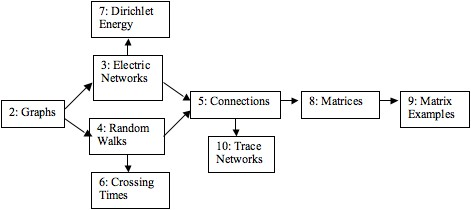
\includegraphics[width=4in]{Dependencies.jpg} 
   \caption{Section dependencies, where $ A\rightarrow B$ means $ A $ is a prerequisite for   $ B $. The prerequisite relation is transitive.}
   \label{Dependencies}
\end{figure}

*** (Needs more info)***  Section dependencies are indicated in Figure~\ref{Dependencies}.   Sometimes there are forward references for alternative proofs, examples, etc.,  but this is minor and not essential to the development.






%%%%%%%%%%%%%%%%%%%%%%%%%%%%%%%%%%%%%%%%%
%%%%%%%%%%%%%%%%%%%%%%%%%%%%%%%%%%%%%%%%%
%%%%%%%%%%%%%%%%%%%%%%%%%%%%%%%%%%%%%%%%%

\newpage\section{\textbf{Introduction}} 

\bigskip Section:
\begin{enumerate}


\item[2]
We introduce the idea of a graph with weights on it edges.

\item[3] We show how the graph can be interpreted as an electrical network, where the weight  on each edge is the conductance, i.e.\ the reciprocal of the resistance, of the corresponding wire.  The current between connected nodes is given by the voltage difference and the conductance, according to Ohm's law. 
Induced voltages are then given by solving Laplace's equation, and this is essentially Kirchoff's law. The normalised current (normalised by total conductance at wires connected to that node) out of a node is the laplacian of the voltage at that node.

We introduce the idea of the effective resistance  $ \mathbb{R}_{ab} $ (the reciprocal is  the effective conductance) between two nodes $ a   $ and $  b $.  We see this corresponds to solving Laplace's equation with $ v(b) = 0 $ and either a pointwise or Laplacian condition at $  a$.  The first is a Dirichlet problem and the second is finding the Green's function --- in the discrete setting as here the two are equivalent and this gives useful information.

We show $ \mathbb{R}_{ab} $ defines a metric.

\item[4] Etc., etc.

%\item[3] In this section we define the random walk RW, a reversible markov chain,  associated with the graph.  

%For fixed $ G \subset V $ and $ a\notin G  $, there are two important functions: the normalised expected number $g(x) = \dfrac{1}{c_x} \mathbb{E}^aV_{x\to G} $ of visits to $ x $   in crossing from $ a  $    to $ G \subset V $,  and the probability $h(x) = P^x(T_a<T_G) $ that the RW from $ x $ reaches $ a $ before  $G $.
%We see both are  harmonic if  $ x\neq a,\, x\notin G $ and hence $ g(x) =  \lambda h(x) $.  

%We know $ h(a) = 1 $, $ g(a) = \dfrac{1}{c_a} \mathbb{E}^aV_{a\to G} $  and \emph{compute} $ -c_a\lap h(a) = c_a P^a (T_G < T_a^+) $, $ -c_a\lap g(a) = 1 $.   Since  $ \lambda  = h(a)/g(a) = -c_a\lap h(a) / -c_a \lap g(a) $ this gives two expressions for $ \lambda $.  Moreover, the first is the reciprocal of the voltage $  g$ for a unit current flow and the second is the current flow for a unit voltage voltage $ h $, and so both equal $ \mathbb{C}_{aG}$.

%
%\item[4] 


\end{enumerate} 


 
%%%%%%%%%%%%%%%%%%%%%%%%%%%%%%%%%%%%%
%%%%%%%%%%%%%%%%%%%%%%%%%%%%%%%%%%%%%
%%%%%%%%%%%%%%%%%%%%%%%%%%%%%%%%%%%%%
%%%%%%%%%%%%%%%%%%%%%%%%%%%%%%%%%%%%%
\section{\textbf{Graphs}}  \label{secint}

\begin{figure}[htbp] %  figure placement: here, top, bottom, or page
   \centering
   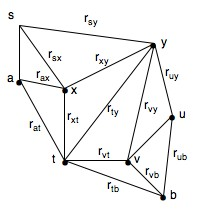
\includegraphics[width=2in]{graph.jpg} 
   \caption{A finite graph}
   \label{graph}
\end{figure}

A \emph{(finite) graph} is a triple
\[  \mathbb{G}  = (V,E, r_{xy} ) \]
where 
\begin{itemize}
\item $ V $ is the finite set of \emph{vertices} or \emph{nodes},
\item $ E $ is the set of \emph{edges} and consists of certain pairs of distinct vertices,
\item $ r_{xy} $ is a (strictly) \emph{positive} function defined on $ E $.
\end{itemize}
Note $ r_{xy} = r_{yx} $.

We assume the graph to be \emph{connected}.

\subsection{Notation and Definitions}
\begin{itemize}
\item Write $ x\sim y $ if $ \{x,y\} \in E $.
\item A \emph{simple} graph is one such that $ r_{xy} \equiv 1 $ for $ \{x,y\}\in E$.
\item  $ c_{xy} := 1/r_{xy}$.    

If $ xy $ is not an edge define $ c_{xy} = 0$.  

$r_{xy} $ is the \emph{resistance} of the edge $ xy$ and $ c_{xy} $ is the \emph{conductance}.

\item The \emph{weighted degree} of $ x $ is $ c_x := \sum_y c_{xy} $.
It is the number of edges from $ x $ if $  \mathbb{G}  $ is simple and in this case is just called the \emph{degree} of $ x $.

\item The \emph{total mass} of $  \mathbb{G}  $ is $ C = C( \mathbb{G} ) := \sum_x c_x $. \label{tm}  In the case of a simple graph it is twice the number of edges, or equivalently the sum of the degrees of the vertices.

\end{itemize} 


%%%%%%%%%%%%%%%%%%%%%%%%%%%%%%%%
%%%%%%%%%%%%%%%%%%%%%%%%%%%%%%%%
%%%%%%%%%%%%%%%%%%%%%%%%%%%%%%%%

\section{\textbf{Electric Network Interpretation of a Graph}}  \label{secEN}

\subsection{Physical Motivation} \label{pm}  Fix the graph $  \mathbb{G}  $.  Think of $  \mathbb{G}  $ as an electric network [EN] with resistance $ r_{xy} $ on each edge $ xy $. Suppose $ \emptyset\neq G \subset V $ and $ a \in V \setminus G $.  
Voltages $ v(a) \neq 0 $, and $ v(b) = 0  $ for $ b \in G $, are imposed.  (That is, the circuit is grounded on $ G $.)  

An important case is $ G = \{ b \} $ contains a single node.  The set of nodes $\{ a\} \cup G   $  is the set of \emph{boundary} nodes.   Later we impose  more general boundary conditions on $ v $.  The \emph{interior} nodes are $ V^\circ = V \setminus G $.

\begin{itemize}
\item
Each node $ x $  settles into a steady state voltage $ v(x) $.
\item A \emph{current} $ i_{xy} $ flows from $ x $ to $ y $ where 
\[ i_{xy} = (v_x - v_y) c_{xy}. \text{\quad \emph{(Ohm's law)}}\]
Thus $ i_{xy} = - i_{yx} $ and current  flows ``downhill''.

\item For $ x  $ an interior node there is \emph{zero net current} flowing out of   $ x $, i.e.\ into $  \mathbb{G}  $ through $ x $:
\[  \sum_y i_{xy}\  \left(\text{i.e.}\ \sum_y (v_x - v_y) c_{xy}\right) = 0.  \text{\quad \emph{(Kirchoff's law)}}\]

 \end{itemize} 
   
%%%%%%%%%%%%%%%%%%%%%%%%
\subsection{Mathematical Framework}\label{mf}
Because of the previous physical motivation%
\footnote{Equation  \eqref{wsum} is a rewriting of Kirchoff's law at $ x $.}  
define  the \emph{voltage}  to be the unique (see below) function $ v $ with%
\footnote{We could as well take $ v(a) < 0 $, but it is convenient to take a positive voltage at $ a $ as we then have a current flowing from $ a $ \emph{into} $ \mathbb{G} $ and then \emph{out of} $ \mathbb{G} $ through $ G $.}
\begin{gather}
 \text{ prescribed } v(a)>0,\quad   v(b)=0 \text{ for } b \in G,
   \label{wbd}  \\
  v(x) = \frac{1}{c_x} \sum_{y\sim x} c_{xy}v(y)  , \quad x\neq a, x \not\in  G.  \label{wsum}
 \end{gather}
  Thus for interior $ x  $, $ v(x) $ is a \emph{weighted average} of $ v $ at neighbouring nodes. 
  
  Note that the second set of boundary conditions and \eqref{wsum} are \emph{homogeneous}, i.e.\ preserved under addition and scalar multiplication of functions. 

\medskip
The following are true for general boundary voltages, with the same proofs.
\begin{itemize}

\item Denote the \emph{Laplacian} of   $ f: V \to \mathbb{R} $  by%
\footnote{So $ \lap f (a)$ is the difference between the weighted average of $ f $ at neighbours of $ a $ and the value $ f(a) $ itself.}
\begin{equation} \label{dlap}    
\boxed{
\triangle f(x) := \left( \frac{1}{c_x} \sum_{y\sim x} c_{xy}f(y) \right) - f(x) =  \frac{1}{c_x} \sum_{y\sim x} c_{xy}\big( f(y) - f(x) \big).
}
\end{equation} 
Thus \eqref{wsum} implies 
\begin{equation} \label{lap}
 \triangle v(x) = 0,   \quad x\neq a, x \not\in  G.
\end{equation} 
For this reason we say $ v $ is  \emph{harmonic}  at interior nodes.

\item \emph{Maximum Principle}:   For interior $  x  $;  $ v(x) \leq \max_{y\sim x} v(y) $ 
by \eqref{wsum}.  Thus 
\begin{equation} \label{maxp}
 0 \leq   v(x) \leq v(a) \text{ for all } x.
\end{equation}

\item \emph{Uniqueness}: Any two solutions of \eqref{wbd} and \eqref{wsum} are equal. 
 (Apply \eqref{maxp} to the difference of  the solutions.) 

\item \emph{Existence}: There \emph{exists} a (unique) solution of \eqref{wsum}. 
(Since uniqueness implies existence for $ n $ linear equations in $ n $ variables.)

\item  The \emph{current} along the (directed) edge   $x y $ is $ i_{xy} :=(v_x-v_y) c_{xy}$. Clearly $ i_{xy} = -i_{yx} $.

\item The \emph{current out of $ x \in V $}, or \emph{into $   \mathbb{G}  $ at $ x $}, is defined by
\begin{equation} \label{ilap} 
\boxed{
i_x := \sum_y i_{xy} = -c_x \triangle v(x).
}
\end{equation} 
Thinking of the case $ i_x< 0 $ ,   $ -i_x $ is the current  \emph{out of $ \mathbb{G} $ at $ x $}.
 
Note $ i_x = 0 $ at interior nodes by~\eqref{lap}. The  \emph{flux} of $ i $ through the network is%
\footnote{\label{fnequ}
Equality comes from
\[
0 = \sum_x \sum_y i_{xy}  
   = \sum_y i_{ay} + \sum_{b\in G}\sum_y i_{by}    =i_a +\sum_{b\in G} i_b,
\]
where the first equality is because $ i_{xy} = -i_{yx} $ and the second because $ i_x=0 $ at interior nodes.
}
\begin{equation} \label{flx}  
F(i) := i_a = -\sum_{b\in G} i_b.
\end{equation} 
\end{itemize}
%%%%%%%%%%%%%%%%%%%%%%%%%%%%%%%%%%%%%%%%%%
\subsection{Rescaling Solutions} \label{rescale} We make a simple but very useful observation which depends essentially on the homogeneity in \eqref{wbd} and~\eqref{wsum}.

If $ f_1 $ and $ f_2 $ are the solutions of 
\eqref{wbd} + \eqref{wsum} with prescribed voltages at $ a $ given by $ f_1(a) $ and $ f_2(a) $ respectively, then trivially by uniqueness and homogeneity, $ f_1 $ and $ f_2 $  are equal up to rescaling:
\begin{equation} \label{scs}
f_1(x) = \frac{f_1(a)}{f_2(a)}f_2(x), \ \forall x .
\end{equation} 
Moreover, 
\begin{equation} \label{lapfr}
 \frac{f_1(a)}{f_2(a)}  =  \frac{\lap f_1(a)}{\lap f_2(a)} .
\end{equation}
So either of the above can be used as the scaling factor in~\eqref{scs}.


%%%%%%%%%%%%%%%%%%%%%%%%%%%%%%%%%%%%%%%%%%
\subsection{Effective Conductance and Resistance}  
The important case is $ G = \{ b \} $.
\begin{itemize} 
 \item Motivated by Ohm's law (see Section~\ref{pm})
the  \emph{effective conductance} and  \emph{effective resistance} between $ a $ and $ G $ are defined by
\begin{equation} \label{effr} 
 \mathbb{C}_{aG} = \frac{1}{\mathbb{R}_{aG}} = \frac{i_a}{v(a) }.
\end{equation} 
Note  $ \mathbb{C}_{aG} $ and  $ \mathbb{R}_{aG} $ are independent of $v(a) $ 
by~\eqref{scs}. 

\item \emph{Symmetry}:%
\footnote{\label{sp}If $ f $ and $ g $ are harmonic so is the linear combination $ h = \alpha f + \beta g $ (\emph{superposition principle}).
The current corresponding to $ h $ along an  edge is then the same linear combination of the currents corresponding to $ f $ and $ g $ along the edge.  If $ f $ is defined by $ f(a) = 1 $ and $ f(b)=0 $ then the current  out of $ a $ is $ \mathbb{C}_{ab} $.  If   $g $ is defined by $ g(a) = 0 $ and $g(b)=1 $ then the current out of $ b $ is $ \mathbb{C}_{ba} $, and  hence out of   $ a $ is $ -\mathbb{C}_{ba} $  by \eqref{flx}.  It follows that the current corresponding to $ h = f + g $ and out of $ a $ is  $ \mathbb{C}_{ab}- \mathbb{C}_{ba} $.  Since $ h(x) =1\ \forall x $ o the current corresponding to $ h $ is zero.}
 \[  \mathbb{C}_{ab} = \mathbb{C}_{ba}, \quad  \mathbb{R}_{ab} = \mathbb{R}_{ba}. \]
 
 \item \emph{Triangle Inequality}: The effective resistance defines a metric on $  \mathbb{G}  $ since 
 \begin{equation} \label{trii}
 \boxed{\mathbb{R}_{ac} \leq  \mathbb{R}_{ab} +  \mathbb{R}_{bc} .}
 \end{equation} 
 \begin{proof}%
 \footnote{I havn't seen this proof before.  It is elementary and gives a precise value for the error term in the triangle inequality.} 
 Let $v_1 $ be the voltage function defined as the harmonic extension of $ v_1(a) = \mathbb{R}_{ab} $ and $ v_1(b) = 0 $.   Let $ i_1 $ denote the corresponding current, a unit flow from $ a $ to $ b $. 
  
 Let $v_2 $ be the voltage function defined as the harmonic extension of $ v_2(b) = 0 $ and $ v_2(c) = -\mathbb{R}_{ac} $.   Let $ i_2 $ denote the corresponding current, which in particular is a unit flow from $ b $ to $ c $. 
  
Let $ v = v_1 + v_2 $ and so the corresponding current is $ i = i_1 +i_2 $.   Then  $ i $ is a unit flow from $ a $ to $ c $ in the sense of~\eqref{fld}, since $ i(a) = i_1(a) + i_2(a) = 1 +0 = 1$, $ i(b) = i_1(b) + i_2(b) = -1+ 1 =0 $ and $ i(c) = i_1(c) + i_2(c) = 0-1 =-1$. 
Notice that $ v $ is harmonic at $ b $ since by \eqref{ilap}
\[
 \lap v(b) = \lap v_1(b) + \lap v_2(b) = -c_b^{-1} (i_1(b) + i_2(b))=0 .
 \]
It follows that $ v $ is the harmonic extension of $ v(a) = \mathbb{R}_{ab} + v_2(a) $ and of $ v(c) = v_1(c) - \mathbb{R}_{ac}  $.  Since $ i $ is a \emph{unit} flow from $ a $ to $ c $ it  follows that $ v(a) - v(c) = \mathbb{R}_{ac}$. 


But  $ v_2(a) \leq 0 $ and $ v_1(c) \geq 0 $ by the maximum principle, and so 
\[
\mathbb{R}_{ac} = v(a) - v(c) = \mathbb{R}_{ab} + \mathbb{R}_{bc} 
           + v_2(a) - v_1(c) \leq \mathbb{R}_{ab} + \mathbb{R}_{bc}.  \qedhere
\]
 \end{proof}
 
We give a random walk proof on page~\pageref{rwp} and a proof using trace networks in  ***  . 
 \end{itemize} 

%%%%%%%%%%%%%%%%%%%%%%%%%%%
\subsection{Computing Effective Conductance}\label{seccer}

\subsubsection{Resistances in parallel and in series}
 Conductances add in parallel, resistances  add in series. 

\begin{figure}[htbp]
   \centering
   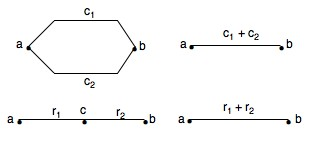
\includegraphics[width=2.5in]{addr.jpg} 
   \caption{Conductances add in parallel, resistances add in series.}
   \label{addr}
\end{figure}


In Figure~\ref{addr} voltages $ v(a), v(b) $ are prescribed, as are conductances $ c_1, c_2 $ and resistances $ r_1, r_2 $.
 In the top two diagrams  
the current flowing from $ a $ to $ b $ is clearly
\[ (v(a)-v(b))(c_1 + c_2). \]
 In the bottom  left diagram  direct calculation shows the induced voltage at $ c $ is 
\[ 
\frac{ \frac{1}{r_1} v(a) + \frac{1}{r_2} v(b) } { \frac{1}{r_1} + \frac{1}{r_2} }.
\]
Easy calculation then shows the current flowing out of $ a $, and the current flowing into $ b $, is 
\[
\frac{v(a) - v(b)}{r_1 + r_2} 
\]
in both of the bottom diagrams. 

It follows that in any circuit the two left side diagrams can be replaced by the corresponding right side diagrams when computing induced voltages, current flow or effective resistance.  They have the same input-output relations on the nodes $ \{ a, b \} $ and so we say they are \emph{equivalent} on the nodes $ \{a, b\} $.  See  also Section~\ref{secbb}.   See [DS, p 44] for an example calculation.

\subsubsection{The $ \Delta  -  Y$   transform}  Consider the two networks in 
Figure~\ref{DeltaY} with conductances as shown.

\begin{figure}[htbp] %  figure placement: here, top, bottom, or page
   \centering
   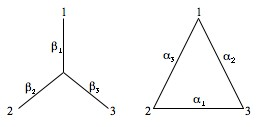
\includegraphics[width=3in]{DeltaY.jpg} 
   \caption{The $ \Delta  -  Y$   transform }
   \label{DeltaY}
\end{figure}

We say they are \emph{equivalent} if they have the same input output relations on the nodes $ \{1, 2, 3\} $.

\begin{proposition}
The networks in Figure~\ref{DeltaY} are equivalent on $ \{1,2,3\} $ iff
\begin{equation} \label{}
\alpha_1 = \frac{\beta_2 \beta_3}{\beta_1 + \beta_2 + \beta_3},\quad 
\alpha_2 = \frac{\beta_3 \beta_1}{\beta_1 + \beta_2 + \beta_3},\quad 
\alpha_3 = \frac{\beta_1 \beta_2}{\beta_1 + \beta_2 + \beta_3}.
\end{equation}
Equivalently, iff 
\begin{equation} \label{}
\beta_i = \frac{S}{\alpha_i},   \text{ where } S = \alpha_1 \alpha_2 +  \alpha_2 \alpha_3 +  \alpha_3 \alpha_1 . 
\end{equation}
\end{proposition} 

\begin{proof}%
\footnote{This is less tedious than computing the effective resistances between the pairs 12, 23 and 31.}
It is sufficient to consider a voltage 1 at node 1 and 0 at nodes 2 and 3, since by symmetry this covers  
two similar cases by rotating, and then all cases by scaling and summing boundary data.

In the $ Y $ diagram, the induced voltage at the central node is $ \beta_1/(\beta_1 + \beta_2 + \beta_3) $.
The currents through 1, 2 and 3 then are:
\[
i_1 = \beta_1 \left(1-\frac{\beta_1}{\beta_1 + \beta_2 + \beta_3}\right) =
            \frac{\beta_1(\beta_2+\beta_3)}{\beta_1 + \beta_2 + \beta_3}, \quad 
            i_2 =  \frac{\beta_1\beta_2}{\beta_1 + \beta_2 + \beta_3},\quad 
             i_3=  \frac{\beta_1\beta_3}{\beta_1 + \beta_2 + \beta_3}
\]
In the $ \Delta $ diagram the corresponding currents are
\[
i_1 = \alpha_3 + \alpha_2, \quad i_2 =  \alpha_3 , \quad i_3 = \alpha_2.
\]
Hence 
\[
  \alpha_2 =  \frac{\beta_1\beta_3}{\beta_1 + \beta_2 + \beta_3},\quad 
            \alpha_3=  \frac{\beta_1\beta_2}{\beta_1 + \beta_2 + \beta_3},
                        \]
and so 
\[
  \alpha_1 =  \frac{\beta_2\beta_3}{\beta_1 + \beta_2 + \beta_3}
                          \]
by symmetry. 

 It follows that 
\begin{align*}
S  := \alpha_1 \alpha_2 +  \alpha_2 \alpha_3 +  \alpha_3 \alpha_1 
= \frac{\beta_1\beta_2\beta_3(\beta_1 + \beta_2 + \beta_3)}{(\beta_1 + \beta_2 + \beta_3)^2}
=  \frac{\beta_1\beta_2\beta_3}{ \beta_1 + \beta_2 + \beta_3  },
\end{align*} 
and so $ \beta_i = S/ \alpha_i $.
\end{proof}
   
\begin{proof}[Alternative Proof]  From the conductance matrix for $Y $, 
\[
A =  \left[ \begin {array}{cccc} -{\beta_1}&0&0&{\beta_1}
\\\noalign{\medskip}0&-{\beta_2}&0&{\beta_2}\\\noalign{\medskip}0&0&-{
\beta_3}&{\beta_3}\\\noalign{\medskip}{\beta_1}&{\beta_2}&{\beta_3}&-{\beta_1 }-{\beta_2}-{\beta_3}\end {array} \right] 
\] 
one can use Maple to compute the trace conductance matrix  $ B $ on $ \Delta$ via~\eqref{trMa}.  Namely,
\[
B =  A_{GG} - A_{GH} A_{HH}^{-1} A_{HG} =
 \left[ \begin {array}{ccc} -{\frac {{\beta_1}\, \left( {\beta_2}+{\beta_3} \right) }
 {{\beta_1}+{\beta_2}+{\beta_3}}}&{\frac {{\beta_1}\,{\beta_2}}
{{\beta_1}+{\beta_2}+{\beta_3}}}&{\frac {{\beta_1}\,{\beta_3}}{{\beta_1}+{
\beta_2}+{\beta_3}}}\\\noalign{\medskip}{\frac {{\beta_1}\,{\beta_2}}{{
\beta_1}+{\beta_2}+{\beta_3}}}&-{\frac {{\beta_2}\, \left( {\beta_1}+{  
\beta_3} \right) }{{\beta_1}+{\beta_2}+{\beta_3}}}&{\frac {{\beta_2}\,{\beta_3}}
{{\beta_1}+{\beta_2}+{\beta_3}}}\\\noalign{\medskip}{\frac {{\beta_1}\,{
\beta_3}}{{\beta_1}+{\beta_2}+{\beta_3}}}&{\frac {{\beta_2}\,{\beta_3}}{{
\beta_1}+{\beta_2}+{\beta_3}}}&-{\frac {{\beta_3}\, \left( {\beta_1}+{  
\beta_2} \right) }{{\beta_1}+{\beta_2}+{\beta_3}}}\end {array} \right].  
\]
\end{proof} 





%%%%%%%%%%%%%%%%%%%%%%%%%%%%%%%%
%%%%%%%%%%%%%%%%%%%%%%%%%%%%%%%%
%%%%%%%%%%%%%%%%%%%%%%%%%%%%%%%%
\section{\textbf{Random Walk Interpretation of a Graph}}\label{rwi}

\subsection{Definition of the RW on  $ \mathbb{G} $ }  This is characterised by defining the probability of moving from $ x $ to $ y $ to be
\begin{equation} \label{}
p_{xy} = \frac{c_{xy}}{c_x}.
\end{equation}
Thus \emph{rows} of the \emph{transition matrix} $ P:= (p_{xy})_{x\in V, y\in V}  $ are probability vectors, with row $ x $ containing the probabilities corresponding to  leaving node $ x $.

\medskip \emph{The RW always begins at time $ 0 $, and its position at time $ n \geq 0 $ is denoted by~$ X_n $.}

 \subsection{Markov Chain}  The random walk is a markov chain with state space $ V   $  and transition probabilities $ p_{xy} $.
\begin{itemize}
\item The markov chain is \emph{irreducible} since $  \mathbb{G}  $ is connected, and so any state can be reached from any other state.  

\item Hence by standard markov chain theory there is a \emph{unique steady state distribution} $ (w_x)_{x\in V } $.

\item As for any markov chain, if $ (u_x)_{x\in V} $ is the probability distribution at one time then $ (v_x)_{x\in V} $, where $ v_x = \sum_y   u_y p_{yx} $, gives the probability distribution at the next time.

\item It follows by direct calculation
 that the \emph{steady state distribution $ w_x $ is proportional to $ c_ x $},%
\footnote{Since if $ w_x:= c_x/C$ then
\[
 \sum_y w_y p_{yx}  = \sum_y \frac{c_y}{C} \frac{c_{yx}}{c_y} = \sum_y\frac{c_{yx}}{C} = 
      \sum_y\frac{c_{xy}}{C} = \frac{c_x}{C} = w_x. 
\]
Hence  $ w_x $ is the steady state distribution by uniqueness.}
 and  so   
\begin{equation} \label{}
 w_x = \frac{c_x}{C}. 
\end{equation} 
      
  \item The markov chain is \emph{reversible}, i.e.
  \[ w_x p_{xy} = w_y p_{yx} \quad  \forall x,y\in V .\]
  
  \item \emph{Interpretation of reversibility}: One cannot tell the direction of time by watching the RW evolve from the steady state distribution $ w $.  More precisely
 \begin{align*}
  P(xy)  := &\  P(X_0=x) \, P(X_1=y | X_0=x)  
  = w_x p_{xy} 
  \\  = &\ w_y p_{yx}   
   =  P(X_0=y) \, P(X_1=x | X_0=y )   =: P(yx).
  \end{align*} 
  
  Similarly 
\begin{align*} 
   P(x_0x_1\dots x_n) &= w_{x_0} p_{x_0 x_1} p_{x_1 x_2} \cdots p_{x_{n-1} x_n}\\
  & = w_{x_n} p_{x_n x_{n-1}} \cdots p_{x_2 x_1} p_{x_1 x_0}
  = P(x_n  \dots x_1x_0 ) .
\end{align*} 
  
  The following equivalent version does not explicitly refer to the steady state distribution.  For any path $ x_0 x_1 \dots x_n $
  and beginning at each end respectively, 
  \[  c_{x_0} P^{x_0}( x_0 x_1 \dots x_n ) =  c_{x_n} P^{x_n}( x_n  \dots x_1x_0 ). \]
  
  \item Conversely, any reversible markov chain is the RW given by a graph, provided we allow $ c_{xx}> 0 $.%
  \footnote{Suppose the markov chain is $ p $ and the steady state distribution is $ w $. Then $ w_x p_{xy} = w_y p_{yx} \ \forall x,y $.  Define $ c_{xy} = w_x p_{xy} $ and note $ c_{xy} = c_{yx} $. Moreover,
  \[ \frac{c_{xy}}{c_x} = \frac{c_{xy}}{\sum_z c_{xz}} = \frac{w_x p_{xy}}{\sum_z w_x p_{xz}} = p_{xy}, \]
  and so this gives the original markov chain.
  }
  
  \item A natural measure on $ V $  is $ (c_x)_{x\in V} $.  The corresponding \emph{transition density}  is defined  for $ x \sim y $ by  
  \[  p(x,y) := \frac{P^x(X_1=y) }{c_y}   = \frac{c_{xy}}{c_x c_y} = \frac{P^y(X_1=x) }{c_x}  = p(y,x).\]
  Reversibility thus is equivalent to symmetry of the transition density $ p(x,y) $ (but \emph{not} of~$ p_{xy} $). 
\end{itemize} 
 
%%%%%%%%%%%%%%%%%%%%%%%%%%%%%%%%%%%
\subsection{Two Functions Associated with the RW}  Suppose $ \emptyset \neq G \subset V $, $ a \in V \setminus G $ and $ x \in V $.  

We introduce two important  functions $ h $ and $ g $ which  equal 0 on $ G $ and are harmonic at $ x \notin \{a\}\cup G $. By the scaling comments in  Section~\ref{rescale}, they are multiples of each other, of the voltage $ v $ in~\eqref{wbd} and~\eqref{wsum}, and of the Green's function discussed later.   We note the consequences in Section~\ref{secER}.  

First some notation.

\medskip
\emph{Notation}:  By $ T_a $ ($ T_G $) is meant \emph{the time of first arrival at $ a $}  ($ G $).  This is from some designated starting point, which in \eqref{dfh} is $ x $.   

By $ V_{x\to G} $ is meant \emph{the number of  visits to $ x $ \underline{before} arriving at $ G $}.     This is from some designated starting point, which in \eqref{dfg} is $ a $.   
 If $ x   $ is the starting point then \emph{the initial visit at time $ 0 $ is included} as a visit to $ x $.  If $ x \in G$ then $ V_{x\to G} = 0 $.

\medskip 
Let
 \begin{gather}
 \boxed{h(x)  = P^x(T_a < T_G),}\label{dfh}\\
\boxed{g(x)  
=  \frac{1}{c_x}\, \mathbb{E}^a (V_{x\to G}).} \label{dfg}
\end{gather}



\begin{proposition}\label{hgprop}
\begin{equation} \label{bchg} 
\begin{gathered}
h(a) = 1,\quad  h(b) = 0\text{ if } b \in G,\\
g(a) = \frac{1}{c_a} \mathbb{E}^a V_{a\to G},
\quad  g(b) = 0\text{ if } b \in G.
\end{gathered} 
\end{equation} 
Moreover,   
\begin{equation} \label{prhar}
\lap h(x) = 0, \quad \lap g(x) = 0 , \quad x \notin \{a\}\cup G.
\end{equation} 
\end{proposition} 

\begin{proof} The boundary conditions are immediate.

\medskip 
Because the start from $ x $ is \emph{followed} by a visit to some  $y \sim  x $,
\begin{equation} \label{} 
h(x)   = \sum_y p_{xy} P^y (T_a < T_G) 
   = \sum_y \frac{c_{xy}}{c_x} \, h(y) ;
\end{equation} 
and because every visit to $ x $ is \emph{preceded} by a visit to some $ y \sim x $,%
\footnote{More precisely, fix $ x \notin \{a\}\cup G $. Then
\begin{align*}
g(x) &= \frac{1}{c_x} \mathbb{E}^a  (V_{x\to G}) 
      =  \frac{1}{c_x} \sum_{n \geq 1} P^a(X_n = x)\quad \text{(as  $x \neq a $) } \\
     &=  \frac{1}{c_x} \sum_{n \geq 1} \sum_{y\sim x} P^a(X_{n-1} = y) p_{yx} 
     =  \frac{1}{c_x}  \sum_{y\sim x} \frac{c_{yx}}{c_y}\, \mathbb{E}^a  (V_{y\to G}) 
     =   \sum_{y\sim x}  \frac{c_{xy}}{c_x}  g(y).
 \end{align*}
    }
\begin{equation} \label{hhg}
 \begin{aligned} 
 g(x) &:= \frac{1}{c_x}   \mathbb{E}^a V_{x\to G} = 
  \frac{1}{c_x} \sum_y p_{yx}\,  \mathbb{E}^a V_{y\to G}\\
 & = \sum_y\frac{1}{c_x}\, \frac{c_{yx}}{c_y} \, c_y\, g(y) =  \sum_y \frac{c_{xy}}{c_y}  g(y).  
\end{aligned} 
\end{equation}   \qedhere
\end{proof}   

Note that \emph{reversibility is required for the proof that $ g $ is harmonic}, but not so for $ h $.


\medskip For later purposes, keeping in mind the scaling comments in Section~\ref{rescale}, we next compute the Laplacians at $ a $. 

Let  $ T^+_a $ denotes the first \emph{return} time to $ a $, i.e.\ the time of the first visit to $ a $ \emph{after} time $ 0$ or equivalently the first visit in positive time. Then
 \begin{equation} \label{} 
 P^a (T_G   < T^+_a )
\end{equation}  
denotes the probability the walk reaches $G$ from $ a $ without returning to $  a $.
It is also called the \emph{escape probability} from $ a $ to $G $.


\begin{proposition}
\begin{equation} \label{laphg} 
-\lap h(a) =    P^a(T_G < T^+_a), \quad  -\lap g(a) = \frac{1}{c_a} .
\end{equation} 
\end{proposition}

\begin{proof}
For $ h $, 
\begin{align*}
- \lap h(a) &= \sum_x\big(h(a) -h(x) \big) p_{ax}  \\
& =\sum_x \big(1-P^x(T_a < T_G)\big)p_{ax} \\
&=\sum_x  p_{ax} P^x(T_G < T_a)  
  = P^a(T_G < T^+_a).
\end{align*}
 
\medskip For $ g $ use  the same calculation as in~\eqref{hhg} after noting
\[
g(a)   := \frac{1}{c_a}   \mathbb{E}^a V_{a\to G} = 
  \frac{1}{c_a} +  \frac{1}{c_a}\sum_y p_{ya}\,  \mathbb{E}^a V_{y\to G},
  \]
where the second equality is because every visit to $ a $ except for the first is preceded by a visit to some~$ y \sim a $.
\end{proof} 

We give a random walk proof of the following. 
It  is also a consequence of the electric network interpretation; see the sentence following \eqref{abi}.
\begin{proposition} \label{receq}For $ a \notin G $,
\begin{equation} \label{epr}  
\boxed{
\mathbb{E}^a  V_{a\to G }  = 1/P^a (T_G < T^+_a).
}
\end{equation} 
\end{proposition} 

\begin{proof}  Let
\begin{align*}
p &= P^a (T_G < T^+_a)  \quad \text{(i.e.\ ``success'')},\\
1-p &= P^a (T^+_a< T_G)  \quad \text{(i.e.\ ``failure'')}.
\end{align*}
The  number of ``failures'' before a success is  a geometric distribution with parameter $ p $.  That is,  the probability of exactly $ n $ returns to $ a $ before reaching $G$, or equivalently exactly $ n+1 $ visits,  is $ (1-p)^n p $.  Hence the expected number of visits to $  a $ before reaching $ G $ is  $1   + $ the mean of the geometric distribution, and  so by a standard result%
\footnote{To see this directly let $ Z $ denote the number of visits to $ a $ before first reaching $ G $. Then 
\begin{align*}
\mathbb{E} (Z) &= \sum_{n\geq 0} (n+1) (1-p)^n p 
 =-p\sum_{n\geq 0} \frac{d}{dp}(1-p)^{n+1}  \\
& = -p \frac{d}{dp}\sum_{n\geq 0}(1-p)^{n+1}   
 = -p\frac{d}{dp}\left(\frac{1-p}{p} \right)  =\frac{1}{p}.
\end{align*}
}
  is $ 1+ (1-p)/p = 1/p$.
  \end{proof} 





 



%%%%%%%%%%%%%%%%%%%%%%%%%%%%%%%%%%%%%%%%%
%%%%%%%%%%%%%%%%%%%%%%%%%%%%%%%%%%%%%%%%%
%%%%%%%%%%%%%%%%%%%%%%%%%%%%%%%%%%%%%%%%%
%%%%%%%%%%%%%%%%%%%%%%%%%%%%%%%%%%%%%%%%%
\section{\textbf{Analysis, Connections with EN and RW}} \label{secER}
Suppose $ \emptyset \neq G \subset V $, $ a \in V \setminus G $ and $ x \in V $.  



\subsection{Green's Function}   \label{secgf}
\subsubsection{Definition} Motivated by the classical situation,%
\footnote{Suppose $ a \in \Omega $.  Then the Green  function $ \mathcal{G}^{\partial \Omega}_a(x) = \mathcal{G}_a (x )$ is characterised  for $x \in  \overline{\Omega} $ by
\begin{align*}
-\lap \mathcal{G}_a(x) &=    \delta_a(x) \quad  \text{if } x \in  \Omega, \quad \text{(Dirac delta measure, equality in distributional sense)}\\ 
 \mathcal{G}_a(x)& = 0 \quad \text{if } x \in \partial \Omega.
 \end{align*} 
 
 In particular, 
 \[
 \mathcal{G}_a(x) = \begin{cases} -\frac{\ln |x-a| }{2\pi} + \psi(x) & n=2, \\
                                                              \frac{c_n}{|x-a|^{n-2}}  + \psi(x) & n \geq 3, \ (c_3 = \frac{1}{4\pi})
                                                              \end{cases}
                                                              \]
 where $ \psi(x) $ is the unique harmonic function on $ \Omega $ such that $  \mathcal{G}_a(x)  = 0$ if $ x \in \partial \Omega$.
  }
\emph{Green's function centred at $ a $} (for the set $G $)  is the unique function 
$ \mathcal{G}^{G}_a  = \mathcal{G}_a:V\to \mathbb{R}  $ given by
\begin{equation} \label{dfgf}
\begin{gathered}
           \boxed{ -\lap \mathcal{G}_a(x) = \dfrac{1}{c_a} \mathcal{X}_a(x),} \quad x \in V\setminus G,\\
            \mathcal{G}_a(x)  = 0 \quad x \in G,
   \end{gathered}
\end{equation} 
where $ \mathcal{X}_a $ is the characteristic function equal to $ 1 $ at $ a $ and $ 0$  elsewhere.
Uniqueness, and hence existence, follow as in Section~\ref{mf}.
Note that $ \dfrac{1}{c_a} \mathcal{X}_a $ is the natural choice as the ``Dirac measure'' centred at $ a $ since it is supported on $ a $ and integrates to $ 1  $ w.r.t.\ the natural measure $ (c_x)_{x\in V }$.

%%%%%%%%%%%%%
\subsubsection{Symmetry} This is analogous to the proof in the classical setting.%
\footnote{Symmetry  of Green's function is shown  for $ a\neq b \in \Omega $ as follows:
 \[
 \mathcal{G}_a(b) - \mathcal{G}_b(a) =
 \int_\Omega \mathcal{G}_b \lap \mathcal{G}_a    - \mathcal{G}_a  \lap \mathcal{G}_b 
 = \int_{\partial \Omega}  \mathcal{G}_b   \frac{\partial \mathcal{G}_a }{\partial \nu}
        -       \mathcal{G}_a   \frac{\partial \mathcal{G}_b }{\partial \nu} = 0
        \]
The first and third equalities are  from the definition of $ \mathcal{G}_a $ and $ \mathcal{G}_b $. The second is  by Green's formula.       Strictly, one should integrate over $ \Omega \setminus (B_\epsilon (a) \cup B_\epsilon (a)) $ and let $ \epsilon \to 0 $.
  }

\begin{equation} \label{} 
\boxed{\mathcal{G}_b(a) =  \mathcal{G}_a(b).} \quad a,b\notin G
\end{equation}
 
\begin{proof}
From Green's identity~\eqref{gi}, which is just an algebraic calculation,
\[  (\lap \mathcal{G}_a, \mathcal{G}_b) = (\mathcal{G}_a, \lap \mathcal{G}_b) ,\]
where each side is the natural inner product with the weighting $ c_x $ at $ x $.  The left side from \eqref{dfgf} is $ c_a \mathcal{G}_b(a) \dfrac{1}{c_a}  = \mathcal{G}_b(a) $ and the right side is similarly $ \mathcal{G}_a(b) $.
\end{proof} 




%%%%%%%%%%%%
\subsubsection{Poisson's equation}  Analogously to the PDE setting,%
\footnote{
The solution of 
\begin{align*}
-\lap u & = f \quad \text{in } \Omega \\
 u &= 0 \quad \text{on } \partial \Omega
 \end{align*} 
 is given by the following ``weighted sum'' of Green functions:
 \[
 u(x) = \int_{\Omega} \mathcal{G}_y(x) f(y)\,  dy.
 \]
 In fact formally, and made precise by a careful limiting argument, one has
 \[
 \int_\Omega \mathcal{G}_y(x) f(y)\, dy 
 = \int_\Omega  \lap_x\mathcal{G}_y(x) f(y)\, dy
 =   \int_\Omega \delta_x(y) \mathcal{G}_y(x) f(y)\, dy = f(x).
 \]
 }
the solution of 
\begin{equation} \label{}
\begin{aligned}
- \lap u (x) &= f (x) \quad x \in V\setminus G, \\
u(x) &= 0 \quad x \in G,
\end{aligned}
\end{equation}
is given by 
\begin{equation} \label{}
\boxed{u(x) = \sum_{y\in V\setminus G} \mathcal{G}_y(x)  f(y)\, c_y.}
\end{equation}
\begin{proof} If $ x \in G $ then
\[
       \sum_{y\in V\setminus G} \mathcal{G}_y(x)  f(y)\, c_y = 0 ,
       \]
 and if $ x \in V \setminus G $ then
\[-\lap_x \left(  \sum_{y\in V\setminus G} \mathcal{G}_y(x)  f(y)\, c_y \right) =
       \sum_{y\in V^\circ} \frac{\mathcal{X}_y(x)}{c_y} f(y) c_y = f(x). \qedhere
       \]
\end{proof}        


%%%%%%%%%%%%%%%%%%%%%%%%%%%%%%%%%%%%%%
\subsection{Summary of Connections so far}
We defined the following functions on $V $, harmonic for $ x \notin G $: 
\begin{align*}
  v(x) &= \text{voltage  given by  \eqref{wbd}, \eqref{wsum}}, \\
h(x) &=P^x(T_a < T_G), \\
 g(x) &= \frac{1}{c_x} \mathbb{E}^a  V_{x\to G},  \\
\mathcal{G}^G_a(x)&= \text{Green function centred at $  a $ given by \eqref{dfgf}}.
\end{align*} 
Moreover, 
\begin{alignat*}{2}
v(a) &=1      &   -c_a\lap v(a)    &= i_a = \mathbb{C}_{aG} \\
h(a) &=1      &   -c_a\lap h(a)   &=  c_a P^a(T_G < T_a^+) \\
g(a) &= \frac{1}{c_a} \mathbb{E}^aV_{a\to G}   &    -c_a\lap g(a)   &=   1\\
\mathcal{G}_a^G(a) &= \text{(no nice analytic expr)}  \quad &    -c_a\lap \mathcal{G}_a^G(a)   &=   1 
\end{alignat*} 

In particular,
\begin{equation} \label{ir1}
 \boxed{v(x) = P^x(T_a < T_G)  
         =  \mathbb{C}_{aG}\,  \frac{ \mathbb{E}^aV_{x\to G} }{c_x} =  \mathbb{C}_{aG}\,  \mathcal{G}^G_a(x)  .}
\end{equation} 
The other information we extract, by using the values of these functions and their Laplacians at $ a $  together with the scaling comments in Section~\ref{rescale}, is
\begin{equation} \label{abi} 
\boxed{\mathbb{R}_{aG} = \frac{1}{i_a} = \frac{1}{c_a P^a(T_G < T_a^+) }
           =  \frac  {\mathbb{E}^aV_{a\to G}}{c_a}  =  \mathcal{G}_a^G(a).   }
\end{equation} 

Note that the third equality above follows directly from the fact that $  g$  and $ h$  are  multiples of each other, and is independent of the direct proof in Proposition~\ref{receq}.


Consider a non empty set of ``boundary'' nodes $   B = \partial V \subset V $.  This generalises the situation in Sections~\ref{secEN}, \ref{rwi} and~\ref{secER}, where $ \partial V = \{a,b\} $ or $ \partial V = \{ a \} $. 


%%%%%%%%%%%%%%%%%%%%%%%%%%%%%%%%%%%%%%
\subsection{Currents and Traverses along Edges} There is also a connection between the current  along an edge and the net number of traverses along the edge.

For this let $ Tr_{xy\to G } $ denote \emph{the \underline{net} number of traverses from $ x  $ to $ y $ before reaching   $G $}.

\begin{proposition} Suppose a voltage is applied at $ a $ and zero voltage is applied at $ G  $, so that \emph{unit} current flows into $ V $  at $ a $.  Then if $ i_{xy} $ denotes the (signed) current along the edge $ xy $,
\begin{equation} \label{}
\boxed{ i_{xy}  = \mathbb{E}^a Tr_{xy\to G} . }
\end{equation} 
\end{proposition} 

\begin{proof}
The voltage $ v(x) $ for unit current flow   is $ g(x) $ as defined in \eqref{dfg}, since both $ v(x) $ and $ g(x) $ are characterised by $ -c_a \lap v(a) = -c_a\lap g(a) = 1 $,
see \eqref{ilap} and  \eqref{laphg}.
Hence
\begin{align*}
i_{xy} &= (g(x)-g(y) )\, c_{xy}  \\
  & = \frac{c_{xy}}{c_x} \mathbb{E}^a(V_{x\to G}) 
     -  \frac{c_{xy}}{c_y} \mathbb{E}^a(V_{y\to G}) 
  =p_{xy}\mathbb{E}^a(V_{x\to G}) 
     -  p_{yx}\mathbb{E}^a(V_{y\to G}) \\
     &=  \mathbb{E}^a(\text{no.\ of traverses from  $ x $ to $ y $ before $ G $})  - 
     \mathbb{E}^a(\text{no.\ of traverses from  $ y $ to $ x $ before $ G $}) \\
     &=  \mathbb{E}^a(\text{\emph{net} no.\ of traverses from  $ x $ to $ y $ before $ G $})
     = \mathbb{E}^a Tr_{xy\to G} . \qedhere
     \end{align*} 
\end{proof}

\emph{Note} that for $ x\sim y $,
\begin{equation} \label{}
g(x)  := \frac{1}{c_x} \mathbb{E}^a  V_{x\to G} = \frac{1}{c_{xy}} \mathbb{E}^a (\text{no.\ of traverses from  $ x $ to $ y $ before $ G $}).
\end{equation} 
The right side is the normalised no.\ of traverses in the direction   $ xy $, \emph{not} the net no.\  of traverses. 





%%%%%%%%%%%%%%%%%%%%%%%%%%%
\subsection{Dirichlet Problem}  Suppose $ G \subset  V $.  (There is here no role played by $ a $.)

Analogous to the classical P.D.E.\ problem%
\footnote{\label{char}Let $ \Omega \subset \mathbb{R}^n $ be  non empty bounded and open with a ``nice'' boundary 
$ \partial \Omega $, e.g.\ $ C^1 $.  
Suppose $h : \partial V \to \mathbb{R}   $ is prescribed and also ``nice'', e.g.\ $ C^1 $.  Then there is a unique harmonic extension of $ h $ to $ \Omega $.   
}
suppose $  h : G \to \mathbb{R}   $ is prescribed.  Then there exists a unique extension of $ h $ to $ V\setminus  G $ satisfying
\begin{equation} \label{}
\lap h(x) = 0  \quad x \notin G .
\end{equation}
Uniqueness, and hence existence, follow as in Section~\ref{mf}.

\medskip
\emph{RW Interpretation}:  (This is analogous to the case of Brownian Motion in the P.D.E.\ setting.%
\footnote{If $ X $ is Brownian motion on $ \Omega $ and $ T_{\partial \Omega} $ is the time of first reaching the boundary, then 
\[
\phi(x) = \mathbb{E}^x \phi(X_{T_{\partial \Omega}}).
\]
})
The solution 
 $ h $   is the expected ``payoff'':
\begin{equation} \label{harw}
 \boxed{h(x) =  \mathbb{E}^xh(X_{T_G} ) .}
\end{equation} 
 where $ {T_G} $ is the time of first arrival at $G $.
 The fact that $ h $ agrees with the given boundary values, and is harmonic   on $V\setminus G $, is given by the same argument as for Proposition~\ref{hgprop}.
 
\medskip \emph{EN Interpretation}:
 It also follows as in Sections~\ref{pm} and \ref{mf} that we can regard $ h $ as giving the voltage  at each node in  $ V $ for  the prescribed voltages on $G $.




%%%%%%%%%%%%%%%%%%%%%%%%%
%%%%%%%%%%%%%%%%%%%%%%%%%
%%%%%%%%%%%%%%%%%%%%%%%%%

\section{\textbf{Crossing Time, Einstein Relation}}
%%%%%%%%%%%%%%%%%%%%%%%%%
\subsection{Crossing Time Theorem}
Note that we do not normally have $ \mathbb{E}^a T_b = \mathbb{E}^b T_a $.   For example, consider a triangular network with nodes $ V = \{a,b,c\} $.  Suppose   $ c_{ab} = c_{ac} = \epsilon $ and $ c_{bc} = 1 $.  Suppose $ \epsilon $ is small.

If the walk starts from $ a $ then $ 1/2$ of  the time it will go directly to $ b $.  The other  $ 1/2 $ it will go to $ c $ and then with probability $  1-\epsilon $ go directly to  $ c $. So   
 \[
  \mathbb{E}^a T_b =  \frac{1}{2} + \frac{1}{2} \, 2 + O(\epsilon) = \frac{3}{2} + O(\epsilon).
  \]
 If the walk starts from $ b$ then it will bounce back and forth many times between $ b $ and $ c $ before reaching $ a $.   In fact for any fixed $ n $, $ \mathbb{E}^b T_a = n - O(\epsilon ) >>  \mathbb{E}^a T_b $.
  
\bigskip  The following was first proved  in [Chandra et al, 1989].
\begin{equation} \label{ctt} 
\boxed{\mathbb{E}^a T_b + \mathbb{E}^b T_a = \mathbb{R}_{ab}\, C( \mathbb{G} ).}
\end{equation} 

\begin{proof}%
\footnote{I have not seen quite this proof before, but it is natural within the current development.
It only uses the facts that $c_x^{-1} \mathbb{E}^a  V_{x\to b} $   is harmonic except at $a  $ and $ b $, its value at $ a $ is $ \mathbb{R}_{ab} $ and  $ \mathbb{R}_{ab} $ is symmetric.}
One has
   \[
\mathbb{E}^a T_b  + \mathbb{E}^b T_a =\sum_x   \left(\mathbb{E}^a  V_{x\to b}  +  \mathbb{E}^b  V_{x\to a} \right)
  \]

From \eqref{abi} and the previously proved $ \mathbb{R}_{ab} = \mathbb{R}_{ba}$, 
$  c_x^{-1}\left(\mathbb{E}^a  V_{x\to b}  +  \mathbb{E}^b  V_{x\to a} \right)$ 
is harmonic with boundary values $ \mathbb{R}_{ab} $ at $ a $ and $ b $.
Hence
\[
  c_x^{-1}\left(\mathbb{E}^a  V_{x\to b}  +  \mathbb{E}^b  V_{x\to a} \right) = \mathbb{R}_{ab} 
\]
for all $ x\in V $.  
It follows that 
\[
\mathbb{E}^a T_b + \mathbb{E}^b T_a  = \mathbb{R}_{ab}\, C( \mathbb{G} ).
 \qedhere
  \] 
\end{proof} 





%%%%%%%%%%%%%%%%%%%%%%%%%%
\subsection{Einstein Relation}
The left side of  \eqref{ctt} is the expected \emph{commute time} from $ a $ to $ b $ and back, $ \mathbb{R}_{ab}$ is the distance between $ a $ and $ b $ in the resistance metric, and $ C = C( \mathbb{G} )$ is the total mass of $ \mathbb{G}  $ (see page~\pageref{tm}).  
This  gives the multiplicative version of the \emph{Einstein relation}:  
\begin{equation} \label{er1}
\boxed{\text{Time} = \text{Distance} \times \text{Mass}.}
\end{equation} 

We often have a ``scale'' or parameter $ x $, such as Euclidean distance, where for appropriate exponents
\begin{equation} \label{dexp} 
 \text{Time} \sim x^{d_w},  
\text{ Distance} \sim x^{d_r}, \text{ Mass} \sim x^{d_f }. 
\end{equation} 
More precisely:  ``Time'' is the commute time between points which are separated by Euclidean distance $\approx  x $,
``Distance'' is the  resistance metric distance  between points which are separated by Euclidean distance $\approx  x $,  and ``Mass'' is the mass of a ball whose Euclidean diameter is $\approx  x $.

The exponents are called the \emph{walk dimension} $ d_w $, the \emph{resistance dimension}  $ d_r $,
and the \emph{fractal dimension}  $ d_f $.  

From \eqref{er1} and \eqref{dexp} one gets the usual form of the \emph{Einstein relation}:
\begin{equation} \label{}
\boxed{d_w = d_r + d_f.}
\end{equation} 


%%%%%%%%%%%%%%%%%%%%%%%%%%%%%%%%%%%%%%%
\subsection{Triangle Inequality} Here is a random  walk proof of the triangle inequality for the resistance metric.  This also gives the error term, see Footnote~\ref{rwet}.

\begin{proof}  \label{rwp} Clearly%
\footnote{\label{rwet}Using an obvious notation, $ T^a_c = T^a_b + T^b_c $  if $T^a_b \leq  T^a_c $ and $ T^a_c = T^a_b - T^c_b < T^a_b + T^b_c$ if $ T^a_c < T^a_b $.  So $ T^a_c \leq T^a_b + T^b_c $ in both cases.

More precisely,
\begin{align*}
\mathbb{E}^a T_c &= P^a(T_b \leq T_c)\, \mathbb{E}^a(T_c \mid T_b \leq T_c )
     + P^a(T_c < T_b)\,  \mathbb{E}^a(T_c \mid T_c < T_b )  \\     
     & = P^a(T_b \leq T_c)\,  (\mathbb{E}^aT_b + \mathbb{E}^bT_c )   + 
          P^a(T_c < T_b)\, \big(\mathbb{E}^aT_b + \mathbb{E}^bT_c - 
                                               (\mathbb{E}^bT_c  + \mathbb{E}^cT_b  )\big)\\
     &=  (\mathbb{E}^aT_b + \mathbb{E}^bT_c ) - P^a(T_c < T_b) \mathbb{E}^b_c ,
\end{align*} 
where $  C^b_c =   C^c_b :=  T^b_c  +  T^c_b $ is the   \emph{commute time} from $  $ to $ c  $ and back to $ b $, and $ \mathbb{E}^b_c := \mathbb{E} C^b_c $.
} 
\[ \mathbb{E}^aT_c    \leq  \mathbb{E}^aT_b + \mathbb{E}^bT_c.
\]
Switching $ a $ and $ c $ and adding,
\[
\mathbb{E}^aT_c  +  \mathbb{E}^cT_a  \leq  \mathbb{E}^aT_b + \mathbb{E}^bT_a + \mathbb{E}^bT_c  + \mathbb{E}^cT_b.
\]
Dividing both sides by $ C( \mathbb{G} ) $ and using the crossing time inequality~\eqref{ctt} gives 
\[    
\mathbb{R}_{ac} \leq \mathbb{R}_{ab}  + \mathbb{R}_{bc} . \qedhere
\] 
\end{proof} 



%%%%%%%%%%%%%%%%%%%%%%%%%%%%%%%%%%%%%%%%%%%
%%%%%%%%%%%%%%%%%%%%%%%%%%%%%%%%%%%%%%%%%%%
%%%%%%%%%%%%%%%%%%%%%%%%%%%%%%%%%%%%%%%%%%%
%%%%%%%%%%%%%%%%%%%%%%%%%%%%%%%%%%%%%%%%%%%
\section{\textbf{Dirichlet Energy}}

\subsection{Definitions}
\begin{itemize}
\item For $ f,g:V\to \mathbb{R} $ define the $\emph{Dirichlet Energy} $ of $ f $, and corresponding bilinear form, by
\begin{equation} \label{def}
\begin{gathered}
\boxed{ \mathcal{E} (f)  = \frac{1}{2} \sum_{x,y} c_{xy}\big(f(x) - f(y)\big)^2, }\\
\boxed{ \mathcal{E}(f,g)  = \frac{1}{2}  \sum_{x,y} c_{xy}\big(f(x) - f(y)\big) \big(g(x) - g(y)\big). }
\end{gathered}
\end{equation} 
The $ \dfrac{1}{2} $ arises since the energy is ``sitting'' on edges, but each edge appears twice in the sum.

\item \emph{EN Interpretation}: If $ f $ is a voltage then $ i_{xy} = c_{xy} (f(x) - f(y) )$ is the current along the  directed  edge $ xy $ and the first summand in~\eqref{def},
\begin{equation} \label{ened} 
   c_{xy}\big(f(x) - f(y)\big)^2 = i_{xy} \big(f(x) - f(y) \big) = i_{xy}^2 r_{xy},
\end{equation} 
 is the ``energy dissipation'' on the edge $ xy $.  The Dirichlet energy  $ \mathcal{E}(f) $ is the ``energy dissipation'' of the network, or equivalently the energy required to keep the network flowing.
 \end{itemize} 
 
 
 %%%%%%%%%%%%%%%%%%%%%%%%%%%%%%%%%%%
 \subsection{Green's Identity}
(This is analogous to the P.D.E.\  case.) 
\begin{equation} \label{gi}
\boxed{\mathcal{E}(f,g) = - (\lap f, g) = -( f,\lap g),} 
\end{equation}
where $ (h,k) = \sum_x h(x) k(x) c_x $ denotes the $ L^2 $ inner product with the 
 natural measure $ (c_x)_{x\in V} $.
 
 In particular, \emph{$ \lap $ is self-adjoint}.
 
Note that \eqref{gi} expresses the energy $ \mathcal{E}(f)$ as a sum of contributions at \emph{nodes} rather than edges, and the  contribution is $ 0 $ at any node where $ \lap f = 0 $ or $ f=0 $.  

Moreover, suppose  $ f $ and $ g  $  are the harmonic extensions of applied voltages on $ G$.  Let $ i^f $ and $ i^g $ denotes   the corresponding currents flowing into $  V  $ on $ G $.  Then \eqref{gi} can be written 
\begin{equation} \label{iof}
\boxed{\mathcal{E}(f,g)  = \sum_{x\in G} f(x)\, i^g(x)=    \sum_{x \in G} i^f(x)\,  g(x)   .}
\end{equation}
 
\begin{proof}[Proof of \eqref{gi}]
\begin{align*}
\mathcal{E}(f,g) &= \frac{1}{2} \sum_{x,y} c_{xy} f(x) \big( g(x) - g(y) \big) 
    - \frac{1}{2} \sum_{x,y} c_{xy} f(y) \big( g(x) - g(y) \big) \\
     &= \frac{1}{2} \sum_{x,y} c_{xy} f(x) \big( g(x) - g(y) \big) 
     + \frac{1}{2} \sum_{x,y} c_{yx} f(x) \big( g(x) - g(y) \big) \\
    &= \sum_{x,y} c_{xy} f(x) \big( g(x) - g(y) \big) = -\sum_x f(x)\, \lap g(x)\, c_x.
    \end{align*} 
\end{proof}
 
%%%%%%%%%%%%%%%%%%%%%%%%%%%%%%%%%%% 
\subsection{Thompson's First Principle}  (This is essentially just a particular case of the standard Dirichlet principle.)
\begin{proposition}
Suppose $h|_{\partial V} $is  prescribed and $ \lap h = 0 $ on $ V^\circ$.  Then
\begin{equation} \label{t11} 
\boxed{\mathcal{E}(h) = \min \{ \mathcal{E}(f) : f=h \text{ on } \partial V\}.}
\end{equation} 
In the case $ \partial V = \{a,b\} $,   $ \lap h = 0 $ on $ V^\circ $, $ h(a) = 1 $ and $ h(b) = 0 $, then 
\begin{equation} \label{t12} 
\boxed{\mathcal{E}(h) = \min \{ \mathcal{E}(f) : f(a)=1, f(b)=0\} = \mathbb{C}_{ab}.}
\end{equation} 
\end{proposition} 

The following proof that the Dirichlet minimiser is harmonic  is analogous to the P.D.E.\ situation.%
 \footnote{(See footnote~\ref{char}.)  The harmonic extension to $\Omega $ of $ h:\partial \Omega \to \mathbb{R} $    is the unique minimiser in $ H^1(\Omega) $ of $ \mathcal{E}(f) := \frac{1}{2} \int_{\Omega} |Df^2 $ with the prescribed boundary conditions.
  Existence comes from taking a minimising sequence and standard P.D.E.\ arguments  to show the sequence converges in the $ H^1 $ sense.   
  
  For here, just note that if $ h $ is harmonic  and $ \phi \in H^1_0(\Omega) $ then 
\begin{align*}
\mathcal{E}(h+\phi) &= \frac{1}{2}\int_{\Omega} |Dh |^2 + 
  \int_{\Omega}  Dh \cdot D\phi  +  \frac{1}{2}\int_{\Omega} |D\phi |^2 \\
&= \mathcal{E}(h)   
  -\int_{\Omega}  \lap h \cdot  \phi  +  \mathcal{E}(\phi) \\
  &= 
  \mathcal{E}(h)    +  \mathcal{E}(\phi)\\
 & \geq  \mathcal{E}(h), \text{ with equality iff $ \phi = 0 $ a.e.}
\end{align*} 
So $ h $ is indeed the unique minimiser.
}
The proof that the Dirichlet energy of the harmonic function is $ \mathbb{C}_{ab} $ follows essentially directly from Green's Identity and the definition of~$ \mathbb{C}_{ab} $.


\begin{proof}  Suppose   $ \phi = 0 $ on $ \partial V $.  Then
\begin{align*}
\mathcal{E}(h+\phi, h+\phi) &= \mathcal{E} (h,h) + 2 \mathcal{E} ( h,\phi) + \mathcal{E}(\phi,\phi)  
                                                  \quad \text{(bilinearity)}\\
&= \mathcal{E}(h,h) - 2 (\lap h,\phi) + \mathcal{E}(\phi,\phi) \quad \text{(Green's identity)}\\
&= \mathcal{E}(h,h)   + \mathcal{E}(\phi,\phi)
\quad \text{(since $ \lap h = 0 $ on $ V^\circ $ and $ \phi = 0 $ on $ \partial V $)}\\
&\geq \mathcal{E}(h,h) 
\end{align*} 
Equality holds in the last line iff $ \phi $ is constant, i.e.\  $ \phi \equiv 0 $. 

This shows that $ h $ is the unique minimiser.


\medskip In the second case, by Green's identity~\eqref{gi},  $ \mathcal{E}(h) =  - c_a \lap h(a) $. 
But  $ - c_a \lap h(a) $ is the current $ i_a $   under the voltage $ h  $, by~\eqref{ilap}.  Since $ h(a) = 1 $ and $ h(b) = 0 $, it follows $ i_a = \mathbb{C}_{ab} $ by the definition of $ C_{ab}$ in~\eqref{effr}. 
\end{proof} 


\subsection{Flows} The following definitions   are motivated by the properties of a current  induced by a voltage applied on $ \partial V $, over a network with possibly unknown conductances.  

\medskip Fix $ \partial V \subset V $.  A \emph{flow} is a function $ j $ on the directed edges of $ \mathbb{G}  $ such that 
\begin{equation} \label{fld}
\begin{aligned}
j_{xy} & = 0   \text{ for } x \not \sim y \\
j_{xy} &= - j_{yx} \\
\sum_y j_{xy} &= 0 \text{ if }x \in V^\circ .
\end{aligned}
\end{equation}


The \emph{flow out of $ x $} for $ x\in V $ (or equivalently \emph{into} $\mathbb{G}  $ at $ x $) is   
\[  j_x := \sum_y j_{xy} . \]
Hence $ j_x = 0 $ if $ x \in V^\circ $.

The \emph{energy} of $ j $ is 
\begin{equation} \label{}
\boxed{\mathcal{E}(j) :=  \frac{1}{2} \sum_{x,y} j_{xy}^2 c_{xy}^{-1}.} 
\end{equation}
This is the same as the energy of $ v $ if $ j $ is the current corresponding to the voltage $ v $.

If $ \partial V = \{ a,b\} $ and $ j_a = -j_b = 1 $, then $ j $ is a \emph{unit flow from $ a $ to $ b $}.



%%%%%%%%%%%%%%%%%%%%%%%%%%%%
\subsection{Properties of Flows}  Suppose $ j $ is a flow and $ w:V \to \mathbb{R} $. Then for any function $ w_x $ ,
\begin{equation} \label{prpf} 
\begin{gathered}
\sum_{x\in \partial V} j_x  = 0, \quad    j_a = -j_b \text{ if }  \partial V = \{ a,b\} , \\
\boxed{\frac{1}{2} \sum_{x,y} (w_x-w_y)j_{xy} =    \sum_{x\in \partial V} w_x j_x .}
\end{gathered} 
\end{equation}
Note the latter is just Green's identity~\eqref{gi}  if $ w= f $ and $ j $ is the current corresponding to the voltage $ g  $.

\begin{proof} The first line follows from the second with $ w_x \equiv 1 $. 

For the second,
\begin{align*} 
\frac{1}{2} \sum_{x,y} (w_x - w_y) j_{xy} &
      =  \frac{1}{2}  \sum_{x,y} w_x j_{xy} -  \frac{1}{2}  \sum_{x,y} w_y j_{xy}  
    =  \frac{1}{2}  \sum_{x,y} w_x j_{xy} -   \frac{1}{2} \sum_{x,y} w_x j_{yx}  \\
 &=  \sum_{x,y} w_x j_{xy}  
   =   \sum_x w_x j_x \\ &=   \sum_{x\in \partial V} w_x j_x. \qedhere
  \end{align*}  
\end{proof} 

%%%%%%%%%%%%%%%%%%%%%%%%%%%%%%%%%%%
\subsection{Thompson's Second Principle} 

\begin{proposition} Suppose $ i $ is the unit flow corresponding to a voltage $ v $ applied to $ a $ and $ b $, with $ v(b) = 0 $.  Then 
\begin{equation} \label{} 
\boxed{\mathcal{E}(i) = \min \{ \mathcal{E}(j) :   j \text{ is a unit flow from $ a $ to $ b $}\} = \mathbb{R}_{ab}.}
\end{equation} 
\end{proposition}

The proof of the following is analogous to that for Thompson's first principle. The value of the minimiser follows from that in the first principle by a simple scaling argument.

\begin{proof}
 For feasible $ j $ let $ j_{xy} = i_{xy} + d_{xy}$.  Then $ d_{xy} $ is a flow with $d_a =d_b = 0 $.
Hence
\begin{align*}
\mathcal{E}(j) &= \frac{1}{2} \sum_{x,y} (i_{xy} + d_{xy})^2 r_{xy} \\
   &= \frac{1}{2} \sum_{x,y} i^2_{xy}r_{xy} + \sum_{x,y}i_{xy} d_{xy} r_{xy} + \frac{1}{2} \sum_{x,y}d_{xy}^2r_{xy}.
   \end{align*}
From~\eqref{prpf} the second term on the right equals
\[ 
\sum_{x,y} (v(x)-v(y)) d_{xy} = 2v(a)  d_a + 2v(b) d_b =0.
\]
Hence 
\[
\mathcal{E}(j) \geq \mathcal{E}(i),
\]
with equality iff $ d = 0 $, i.e.\ $ i=j $.

\medskip

If a unit current flows from $ a $ to $ b $ the applied voltage is $  \mathbb{R}_{ab} $, by the definition of $\mathbb{R}_{ab} $. 
But if the applied voltage is $ 1 $ then the Dirichlet energy is $  \mathbb{C}_{ab} $ from Thompson's first principle.  
Hence if the applied  voltage is $ \mathbb{R}_{ab}  $   the Dirichlet energy is multiplied by $  \mathbb{R}_{ab} ^2 $  from the definition~\eqref{def} of Dirichlet energy, since all voltages will then also be scaled up by $ \mathbb{R}_{ab}  $.
That is, 
\[ \mathcal{E}(i) = \mathbb{R}_{ab}^2 \mathbb{C}_{ab} = \mathbb{R}_{ab} .
\qedhere 
\]
\end{proof} 


%%%%%%%%%%%%%%%%%%%%%%%%%%%%%%%

\subsection{Alternative Expression for Dirichlet Energy}

It is convenient for calculations and otherwise to write $ \mathcal{E}(f,g) $ as a bilinear form in the standard manner, using a positive semi definite matrix.  This will give a slightly different, but more useful, way of expressing the formula for harmonic extensions and for Green's function.  In particular, we do this in Section~\ref{secTN} concerning trace networks. 

\medskip Note: 
\begin{enumerate}
\item $ \mathcal{E}(f,g)  = \frac{1}{2} \sum_{x,y} c_{xy} (f_x-f_y)(g_x-g_y)$ defines a positive semi definite symmetric bilinear form, and $ \mathcal{E}(f,f) = 0 $ iff $ f $  constant.%
\footnote{Think of the graph of $ \mathcal{E}(f,f) $ as  an  $ n-1 $ dimensional parabola $ \times $ straight line, sitting on $ \mathbb{R}^n$, where $ n $ is the cardinality of $ V $.}

\item  
The terms $ c_{xx}$ are zero.
 Replacing $ c_{xx} $  by any other value will not alter the value of~$ \mathcal{E}(f,g) $.  
 
 \item As for any (positive semi definite) symmetric bilinear form,   $ \mathcal{E}(f,g) =  f^T B g = g^T B f$ for some (positive semi definite) symmetric matrix $ B $.
 
 \item Formula \eqref{de2} expresses the energy as a sum of contributions from   \emph{nodes} rather than edges.

 \end{enumerate} 
 
  In the following note that $ -A $ is the positive semi definite matrix.
   $ A $ is often called a \emph{generator  matrix}.%
  \footnote{It is the infinitesimal generator for the associated continuous time Markov process.   ***Elaborate on this somewhere***} 
\begin{proposition}
Let $ A = (a_{xy}) $  for $ x,y \in V $, where 
\begin{equation} \label{defA}
a_{xy} = \begin{cases} c_{xy} & x \neq y \\
                                          -c_x   & x = y 
               \end{cases}.
 \end{equation}
Then 
\begin{equation} \label{de2}
\boxed{\mathcal{E}(f,g) = -\sum_{x,y} a_{xy} f_x g_y}  \ (=  -f^TAg = -g^TAf). 
\end{equation} 
\end{proposition} 

\begin{proof}
 \begin{align*}
\mathcal{E}(f,g) &= \sum_{x,y} c_{xy}f_x g_x - \sum_{x,y} c_{xy} f_x g_y \quad  
                            \text{(since  $ c_{xy}= c_{yx}$)} \\
   &= \sum_{x} c_x f_x g_x - \sum_{\substack{x,y \\ x\neq y}} c_{xy}f_x g_y \quad 
                                         \text{(since  $ c_{x}= \sum_y c_{xy}$ and $ c_{xx} = 0 $)} \\
   &= -\sum_{x} a_{xx} f_x g_x - \sum_{\substack{x,y \\ x\neq y}} a_{xy}f_x g_y\\
   &= -\sum_{x,y} a_{xy} f_x g_y.
\end{align*}
\end{proof} 

%%%%%%%%%%%%%%%%%%%%%%%%%%%%%%%%%%%
\subsection{Cuts and Shorts}





%%%%%%%%%%%%%%%%%%%%%%%%%%%%%%%%
%%%%%%%%%%%%%%%%%%%%%%%%%%%%%%%%
%%%%%%%%%%%%%%%%%%%%%%%%%%%%%%%%
\section{\textbf{Graphs and Random Walks}  (after \cite{Bar3})}

\emph{Here we follow and expand a little on the summary in \cite{Bar3}.} 

\subsection{Graphs}
Let 
\[
 \Gamma = (G,E, a_{xy} \text{ for } \{x,y\}\in E ),
 \] 
 be a finite or infinite \emph{weighted graph} with set of vertices $ G $ and set of edges $ E $.
The weights satisfy 
\[
a_{xy}\geq 0, \quad a_{xy} >0 \text{ iff } x \sim y .
\]
where $ x\sim y $ iff $ \{x,y\} $ is an edge.

\medskip
The \emph{mass} at  $ x $ is 
\[
\mu_0(x) := \sum_y a_{xy },
\] 
and this is extended to a measure $ \mu_0 $ on $ G $.

It is assumed $ \mu_0(x) < \infty $ for all $ x\in G $, which is clearly true if $ G $ is finite.

\medskip The \emph{Laplacian} is defined by
\[
\lap f(x)  =  \sum_y  \frac{a_{xy}}{\mu_0(x) } \big( f(y) - f(x) \big)  
               =    \left( \sum_y  \frac{a_{xy}}{\mu_0(x) }   f(x) \right) - f(x ),
\]
i.e.\ the difference between the weighted average of $ f $ at vertices $ y $ connected to $ x $ and the value of $ f $ at $ x $.

\medskip The \emph{Dirichlet form} is defined by 
\begin{align*}
\mathcal{E} (f,g) &= \frac{1}{2} \sum_{x,y} a_{xy} \big( f(x) - f(y) \big) \big( g(x) - g(y) \big) \quad \text{(sum of energy over all edges in case $ f=g $)}\\
     &=  \sum_x \left( \sum_y a_{xy} \big( f(x) - f(y) \big) \right) g(x) \quad \text{(easy algebra)}\\
     &= (-\lap f,g)_{L^2(\mu_0)}.
     \end{align*} 

%%%%%%%%%%%%%%%%%%%%%%%%%%%%%%%%
\subsection{Random Walk and Markov Chain}

The \emph{discrete time} random walk $ X_n $ is defined with transition probabilities from $ x $ to $ y $ given by 
\[ \mathbb{P} ^x (y) = \frac{a_{xy}}{\mu_0(x)}. \]
 We also write 
\[
 P = (P_{xy}) , \text{ where } P_{xy} = \mathbb{P} ^x (y) ,
 \]
  for the corresponding probability matrix.  So
  \[ 
  (Pf )(x)=  \mathbb{E} ^x f(X_1).
  \]
    Note that 
  \[ 
  \lap = P - I \text{ (i.e.\   $ \lap f = (P-I) f $ with $ f $ a column vector)}; \quad \lap f (x)= \mathbb{E} ^x f(X_1) - f(x). 
  \]

\medskip The \emph{continuous time} random walk $ Y_t $ has jump times given by a Poisson process with parameter $ \lambda $, where usually $ \lambda = 1 $.  (Thus the expected number of jumps in a unit time interval is $ \lambda $.)  When at $ x $ the process jumps to each  neighbour   vertex $ y $  with probability $ \mathbb{P} ^x(y) $.

\medskip
 Thus, with $ P^n $ denoting the $ n $th power of $ P $,  
 \begin{align*}
 \mathbb{P} ^x (X_n = y) &= (P^n)_{xy}  =: P^n(x,y), \\
               \mathbb{P} ^x (Y_t = y) &= \sum_{n \geq 0 } e^{-\lambda  t } \frac{(\lambda  t)^n}{n!} (P^n)_{xy}  =: Q_t(x,y),
 \end{align*}
since the probability of exactly $ n $ jumps in $ [0,t] $ is   $ e^{-\lambda  t } (\lambda  t)^n/n!  $.

Note that 
\[
Q_t =  \sum_{n \geq 0 } e^{-\lambda  t } \frac{(\lambda  t)^n}{n!}  P^n = e^{ - \lambda t+  \lambda t P } = e^ {\lambda t \lap },
\quad  (Q_t f )(x)=  \mathbb{E} ^x f(Y_t).
\]
So $ \lap $ (if $ \lambda = 1 $) is the infinitesimal generator of $ Y $.

\medskip The transition matrix $ P $ is not symmetric.  It is more convenient to work with the   \emph{transition \underline{density}} or \emph{heat kernel} for $ X  $:
\[
p(x,y) := \frac{\mathbb{P}  ^x(y)}{\mu_0(y)} = \frac{a_{xy}} { \mu_0(x)\, \mu_0(y)},
\]
which clearly is symmetric.  More generally
\[
p_0(x,y) = \frac{\delta (x,y)}{\mu_0(y)}, \quad 
p_n(x,y) := \frac{\mathbb{P}  ^x(X_n=y)}{\mu_0(y)} = \frac{\sum_{x_1, \dots , x_{n-1}} a_{x x_1}\cdot a_{x_1x_2} \cdot \ldots \cdot  a_{x_{n-1}y}} { \mu_0(x)\, \mu_0(y)},
\]
which is again symmetric.
Using $ \lap = P - I $, or directly, it is straightforward  to check that $ p_n  $ satisfies the \emph{discrete heat equation}
\[
p_0(x,y) = \frac{\delta (x,y)}{\mu_0(y)}, \quad p_{n+1}(x_0,x) - p_n(x_0,x) = \lap_x p_n(x_0,x) , \quad n\geq 0 .
\]

\medskip
Similarly define the  \emph{transition \underline{density}} or \emph{heat kernel} for $ Y  $:
\[
q_0(x,y) := \frac{\delta (x,y)}{\mu_0(y)} = p_0(x,y), \quad 
q_t(x,y)  :=  \frac{\mathbb{P}  ^x(Y_t = y)}{\mu_0(y)}  
   = \sum_{n \geq 0 } e^{-\lambda  t } \frac{(\lambda  t)^n}{n!}\, p_n(x,y)  \text{ if }t >0,
 \]
which is again symmetric.  
It follows that $ q_t $ satisfies the heat equation
\[ 
q_0(x,y) := \frac{\delta (x,y)}{\mu_0(y)} , \quad \frac{\partial q_t}{\partial t}(x_0,x) = \lap_x q_t(x_0,x).
\]  
Estimates for $ p_n $ transfer easily to $ q_t $.



  


%%%%%%%%%%%%%%%%%%%%%%%%%%%%%%%%
%%%%%%%%%%%%%%%%%%%%%%%%%%%%%%%%
%%%%%%%%%%%%%%%%%%%%%%%%%%%%%%%%
\section{\textbf{Matrices}}


%%%%%%%%%%%%%%%%%%%%%%%%%%%%%%

\subsection{Notation} Consider   $ G\subset V $ and let $ H = V \setminus G $.

Typically one has a sequence of vertices $ (V_n)_{n\geq 0 } $ of prefractal approximations    to a fractal.  One takes $ V=V_{n} $ and either $ G = V_{n-1} $, or $  V_0 $, or $ a $ for some $ a\in V_0 $, or some subset of $ V_0 $.
 
For $ f:V\to \mathbb{R} $ let $ f_G $ and $ f_H $ denote the restrictions to $G $ and  $ H $ respectively.

With $ A $ as in \eqref{defA} write 
\begin{equation} \label{}
A=  \begin{bmatrix} % or pmatrix or bmatrix or Bmatrix or ...
       A_{GG} & A_{GH} \\
      A_{HG} & A_{HH} \\
   \end{bmatrix},
\end{equation} 
with an obvious notation.

\medskip
Let $ D$ be the \emph{diagonal matrix} $ D_{xy}   = c_x  \delta_{xy} $.  Let $ D_G $ and $ D_H $ be the restrictions of $D  $ to $ G $ and $ H $ respectively. 

Let $ P $ be the standard \emph{transition matrix} $ P_{xy} = c_{xy}/c_x $.

Then the \emph{Laplacian} is 
\begin{equation} \label{lapp}
\boxed{ \lap = P-I  .}
\end{equation} 

It follows%
\footnote{Note that for any matrix $ B $ with the same number of rows as $ D $, $  DB $ is obtained from $ B $ by multiplying all terms in row $ i $ by $ D_{ii} $.  Similarly, if  $ B $ has the same number of columns as $ D $ then  $  BD $ is obtained from $ B $ by multiplying all terms in column $ j $ by $ D_{jj} $.}
\begin{equation} \label{APQ}
\boxed{ A =   D(P-I)=   D \lap .}
\end{equation} 
Note that $ A $ is symmetric, but $ \Delta $ and $ P $ are not.






%%%%%%%%%%%%%%%%%%%%%%%%%%%%%%
\subsection{Harmonic Extensions}   
\begin{proposition}
Suppose $ f_G = g $ is prescribed and $ f_H = h $ is the extension to $ H $ such that $ f $ is harmonic on $ H $.
Then
 \begin{equation} \label{harm} 
\boxed{ h= -A_{HH}^{-1} A_{HG}\, g.}
  \end{equation}
  In this case,
 \begin{equation} \label{trMa}
\boxed{ \mathcal{E}(f) = -g^T(A_{GG} - A_{GH} A_{HH}^{-1} A_{HG})g. }
\end{equation}
 \end{proposition} 

\begin{proof} Proceed in the standard manner.  
\footnote{Consider the minimum of $ a g^2 + 2bgh + c h^2 $ for a fixed scalar $ g $   and variable scalar $ h $.  The derivative is zero at $ 2bg + 2ch = 0 $.  Substituting  $ h= -c^{-1}b  $   
the minimum value is $   (a-b^2c^{-1})g^2$.}
(Alternatively, since we know that the minimiser is harmonic we  can also argue directly as in the Remark following the proof.)
\begin{align}
-\mathcal{E}(f) &= 
 \begin{bmatrix} % or pmatrix or bmatrix or Bmatrix or ...
      g^T & h^T \\
   \end{bmatrix} 
 \begin{bmatrix} % or pmatrix or bmatrix or Bmatrix or ...
       A_{GG} & A_{GH} \\
      A_{HG} & A_{HH} \\
   \end{bmatrix}
\begin{bmatrix} % or pmatrix or bmatrix or Bmatrix or ...
      g  \\ h           \\
   \end{bmatrix}    \notag \\
&= g^TA_{GG}g + g^T A_{GH} h + h^T A_{HG} g + h^T A_{HH} h \quad \text{(sum of scalars)}  \notag\\
&= g^TA_{GG}g + 2g^T A_{GH} h + h^T A_{HH} h \quad \text{(take transpose of previous third term)}. \label{enexp}
   \end{align} 
 Since the minimum of $  \mathcal{E}(f) $ occurs at  $ h $, replace $ h $ by $ h+t\phi  $, differentiate w.r.t.\ $ t $, and set $ t=0 $ to get, $ \forall \phi:H\to \mathbb{R}$,
\[
0 = 2 g^T A_{GH} \phi + h^T A_{HH}\phi + \phi^T A_{HH} h   
   =   2 g^T A_{GH} \phi + 2h^T A_{HH}\phi .
\]   
It follows $ g^T A_{GH}  +  h^T A_{HH}= 0 $, so $ A_{HG}g + A_{HH}h = 0  $, and so 
\[ h = - A_{HH}^{-1}A_{HG}g.\]   
   
  Substituting into  ~\eqref{enexp} gives 
\begin{align*} 
 - \mathcal{E}(f) &= g^T(A_{GG} - 2g^TA_{GH}A_{HH}^{-1}A_{HG} + 
                  A_{GH}A_{HH}^{-1}A_{HH}A_{HH}^{-1}A_{HG}) g\\
                  &= g^T(A_{GG} - A_{GH} A_{HH}^{-1} A_{HG})g. \qedhere
 \end{align*} 
      \end{proof} 
      

 \medskip
\emph{Remark}:  We can also obtain \eqref{harm} buy using the fact $ h $ is harmonic.  
That is, from~\eqref{APQ} the equations for the harmonic extension $ f = \begin{bmatrix}  g\\  h    \end{bmatrix} $ of $ g $ can be written
\[
\begin{bmatrix} % or pmatrix or bmatrix or Bmatrix or ...
      I_G & O_{GH} \\
      D_H^{-1} A_{HG} & D_H^{-1} A_{HH} \\
   \end{bmatrix} 
   \begin{bmatrix} g\\ h \end{bmatrix}
   =    \begin{bmatrix} g\\ 0 \end{bmatrix}
\]
Hence 
\begin{align*}
  D_H^{-1} (A_{HG} g + A_{HH} h ) &= 0\\
\therefore\ h &= -A_{HH}^{-1} A_{HG}\, g.
\end{align*} 

%%%%%%%%%%%%%%%%%%%%%%%%%%%%%
\subsection{Green's Function}  
\begin{proposition}
Let  $  \mathcal{G}^G_a(x) $  be the Green function as in Section~\ref{secgf}.  Let   $  \mathcal{G}^G $ be the square matrix with column $ a $ denoted by  $     \mathcal{G}^G_a $  and whose entries are $   \mathcal{G}^G_a(x) $ 
for $ x \in H $.

Then 
\begin{equation} \label{matG}
\boxed{ \mathcal{G}  = -A_{HH}^{-1}. }
\end{equation}
\end{proposition}

\begin{proof} 
 \begin{align*}
   &(I_{H} -P_{HH} ) \mathcal{G}_a  = \dfrac{1}{c_a} \mathcal{X}_a  \quad 
                      \text{(from \eqref{lapp} and \eqref{dfgf})}  \\
\therefore\ &(I_H -P_{HH}) \mathcal{G}  = D_H^{-1}  \quad \text{(by definition of $D  $)}\\
\therefore\ &\mathcal{G}   = (I_H - P_{HH})^{-1} D_H^{-1} = -A_{HH}^{-1}    \quad \text{(by \eqref{APQ})}.
\qedhere
\end{align*}
\end{proof} 

%%%%%%%%%%%%%%%%%%%%%%%%%%%%%%%%%%%%
\subsection{Other Quantities}
\begin{enumerate}

\item \emph{Resistance Metric}: Let $ G=\{y\} $. Then from  \eqref{abi}, $  \mathbb{R}_{xy} = \mathcal{G}_x^{\{y\}}(x) $, 
and so from~\eqref{matG},
\begin{equation} \label{eqcrm}
\boxed{ \mathbb{R}_{xy} =  -(A_{HH}^{-1})_{xx}  \text{ if } G = \{y\}.  }
\end{equation} 



\item  \emph{Visit Times}: Let $ \widetilde{P} $ be the transition matrix for the RW with \emph{absorbing states} $ G $.  Then clearly
$ 
-D^{-1}A_{HH} =   I_{HH}-\widetilde{P}  
$ 
and so 
\[
-A_{HH}^{-1} D = ( I_{HH}-\widetilde{P} )^{-1} =
I_{HH} + \widetilde{P} + \widetilde{P}^2 + \cdots + \widetilde{P}^k + \cdots   
\]
Since $ 
  \widetilde{P}^k_{xy} = P^x(\text{RW is at $ y$  after $ k $ steps}),
$ 
the $ xy $ element of the right side is $ \mathbb{E} ^xV_{y\to G} $.  Hence
\begin{equation} \label{}
\boxed{\mathbb{E} ^xV_{y\to G} = - c_y (A_{HH}^{-1})_{xy}.}
\end{equation} 

\item \emph{Crossing Times}: Since $ \mathbb{E}^x T_G = \sum_y \mathbb{E}^x V_{y\to G}$,
\begin{equation} \label{}
\boxed{ \mathbb{E}^xT_G = - \sum_y c_y (A_{HH}^{-1})_{xy}. }
\end{equation}

\end{enumerate}   



%%%%%%%%%%%%%%%%%%%%%%%%%%%%%%%%
%%%%%%%%%%%%%%%%%%%%%%%%%%%%%%%%
%%%%%%%%%%%%%%%%%%%%%%%%%%%%%%%%
\section{\textbf{Matrix Examples}}

All computations done in Maple.  See accompanying worksheet.



%%%%%%%%%%%%%%%%%%%%%%%%%%%
\subsection{Simple Triangle   T  }

Consider the triangle network $ \{1,2,3\} $ with unit resistances in Figure~\ref{SG(2)H}.   
\begin{figure}[htbp] %  figure placement: here, top, bottom, or page
   \centering
   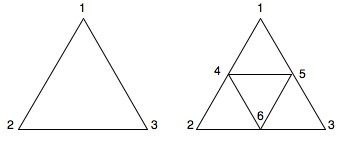
\includegraphics[width=1.5in]{SG(2)H.jpg} 
   \caption{The triangle $ T $ and the $ SG(2)$  prefractal}
   \label{SG(2)H}
\end{figure}


Then 
\[ A =  \left[ \begin {array}{ccc} -2&1&1\\\noalign{\medskip}1&-2&1
\\\noalign{\medskip}1&1&-2\end {array} \right] 
\]

With $ G = \{1\} $, 
\[
 -A_{HH}^{-1} =  \left[ \begin {array}{cc} 2/3&1/3\\\noalign{\medskip}1/3&2/3
\end {array} \right] 
\]
Going down the diagonal, the effective resistances are 
\[
 \mathbb{R}_{12} =\mathbb{R}_{13} = 2/3 .
 \]
The expected crossing times from $ x $ to $ 1$  are obtained by multiplying the elements of column $ x$  by the degrees of the elements and summing: \label{Tq}
\[ \mathbb{E}^2T_1 = \mathbb{E}^3T_1 = 2 . \] 

With $ G = \{1,2\} $,
\[ 
-A_{HH}^{-1}  =   \frac{1}{2} .
\]
So 
\[
 \mathbb{E}_{\{1,2\}3} = \frac{1}{2}, \ \mathbb{E}^3T_{\{1,2\}} = 2 \times \frac{1}{2} = 1 ,
\]
as is clear anyway.

The crossing time theorem  $ \mathbb{E}^1T_2 +  \mathbb{E}^2T_1  = \mathbb{R}_{12}\, C( \mathbb{G} )=4 $ is satisfied.


%%%%%%%%%%%%%%%%%%%%%%%%%%%
\subsection{SG(2) Prefractal} \label{secsg2}  The network is shown in Figure~\ref{SG(2)H}.  Each of the 6 edges is given unit resistance.

%\begin{figure}[htbp] %  figure placement: here, top, bottom, or page
%   \centering
%   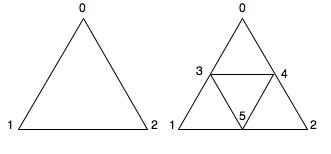
\includegraphics[width=3in]{SG(2).jpg} 
%   \caption{The $ SG(2)$  prefractal}
%   \label{SG(2)}
%\end{figure}

Then
\begin{equation} \label{ASG2}
A =  \left[ \begin {array}{cccccc} -2&0&0&1&1&0\\\noalign{\medskip}0&-2&0&
1&0&1\\\noalign{\medskip}0&0&-2&0&1&1\\\noalign{\medskip}1&1&0&-4&1&1
\\\noalign{\medskip}1&0&1&1&-4&1\\\noalign{\medskip}0&1&1&1&1&-4
\end {array} \right] ,
\quad 
\end{equation} 
We consider the three cases $G = \{1\}, \{1,2\}, \{1,2,3\} $. Then one computes respectively:
\begin{equation} \label{3ahh}
\begin{gathered} 
-A_{HH}^{-1} = 
 \left[ \begin {array}{ccccc} {\frac {10}{9}}&5/9&5/9&4/9&2/3
\\\noalign{\medskip}5/9&{\frac {10}{9}}&4/9&5/9&2/3
\\\noalign{\medskip}5/9&4/9&{\frac {11}{18}}&{\frac {7}{18}}&1/2
\\\noalign{\medskip}4/9&5/9&{\frac {7}{18}}&{\frac {11}{18}}&1/2
\\\noalign{\medskip}2/3&2/3&1/2&1/2&5/6\end {array} \right], \\
 \left[ \begin {array}{cccc} 5/6&1/6&1/3&1/3\\\noalign{\medskip}1/6&1/
3&1/6&1/6\\\noalign{\medskip}1/3&1/6&{\frac {13}{30}}&{\frac {7}{30}}
\\\noalign{\medskip}1/3&1/6&{\frac {7}{30}}&{\frac {13}{30}}
\end {array} \right] ,
\qquad 
 \left[ \begin {array}{ccc} 3/10&1/10&1/10\\\noalign{\medskip}1/10&3/
10&1/10\\\noalign{\medskip}1/10&1/10&3/10\end {array} \right] .
\end{gathered}
\end{equation} 

In particular
\begin{align*}
\mathbb{R}_{12}  = \mathbb{R}_{13}    & = 
                                      \frac{10}{9}  \text{ (first matrix, first 2 diagonal elements)}\\
\mathbb{E}^2T_1 = \mathbb{E}^3T_1 &=  10 \text{ (first matrix, first two columns  $ \times $ corresponding conductances)}\\
\mathbb{R}^3_{\{1,2\}}    &=  \frac{5}{6}   \text{ (second matrix, first  diagonal element)}\\
\mathbb{E}^3 T_{ \{1,2\}} &      = 5 \text{ (second matrix, first column   $ \times $ corresponding conductances)}\\
C\mathbb{G} ) &=   3 \times 2 + 3\times 4  = 18.
\end{align*} 
The crossing time theorem  $ \mathbb{E}^2T_1 +  \mathbb{E}^1T_2 = \mathbb{R}_{12}\, C( \mathbb{G} ) = 20$ is again satisfied.



\medskip
\emph{Mass, Time and Resistance Scaling}:  \label{sc2} Since edges all have unit resistance, i.e.\  the network is simple, the mass is $ \sum_x \text{degree}(x) $, or equivalently twice the number of edges, or equivalently 6 times the number of triangles, i.e.\ 18. But the mass of $ T $ is 6.  So the mass scaling $ m $ is \mbox{$ 18/6 = 3$}.

Next compare the crossing  times and effective resistances above with those for $ T $ on page~\pageref{Tq}. 
Let  $ \tau $ and $ \rho $, respectively, denote the factors by which 
 the  walk times and resistance between comparable nodes scale up in passing from $ T $ to $ SG(2) $.
 
 Then 
$  m = 18/6=3$, $ \tau = 10/2 \text{ or }    5/1 = 5$,
and $  \rho =   \frac{10}{9}\Big/\frac{2}{3} \text{ or } 
                                     \frac{5}{6}\Big/\frac{1}{2}      =\frac{5}{3}$.
That is:
\begin{equation} \label{rssg2} 
\boxed{m = 3,\  \tau = 5,\  \rho = 5/3.}
\end{equation} 
 
 Note the Einstein relation
$  \tau = m \times \rho $ 
holds.                                     


%%%%%%%%%%%%%%%%%%%%%%%%%%%
\subsection{SG(3) Prefractal}  \label{secsg3} The network is shown in Figure~\ref{SG(3)H}.  Each of the 18 edges is given unit resistance.


\begin{figure}[htbp] %  figure placement: here, top, bottom, or page
   \centering
   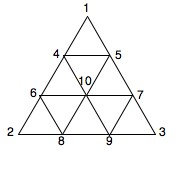
\includegraphics[width=1.5in]{SG(3)H.jpg} 
   \caption{The $ SG(3)$  prefractal}
   \label{SG(3)H}
\end{figure}

We consider the cases   $ G = \{1\},  \{1,2\} $. Then one computes:
\begin{equation} \label{ASG3} 
A =
 \left[ \begin {array}{cccccccccc} -2&0&0&1&1&0&0&0&0&0
\\\noalign{\medskip}0&-2&0&0&0&1&0&1&0&0\\\noalign{\medskip}0&0&-2&0&0
&0&1&0&1&0\\\noalign{\medskip}1&0&0&-4&1&1&0&0&0&1\\\noalign{\medskip}
1&0&0&1&-4&0&1&0&0&1\\\noalign{\medskip}0&1&0&1&0&-4&0&1&0&1
\\\noalign{\medskip}0&0&1&0&1&0&-4&0&1&1\\\noalign{\medskip}0&1&0&0&0&
1&0&-4&1&1\\\noalign{\medskip}0&0&1&0&0&0&1&1&-4&1\\\noalign{\medskip}0
&0&0&1&1&1&1&1&1&-6\end {array} \right],
\end{equation} 
and  
\allowdisplaybreaks{
\begin{gather*}A_{HH}^{-1} =  
\left[ \begin {array}{ccccccccc} {\frac {10}{7}}&5/7&{\frac {11}{21}}
&{\frac {10}{21}}&{\frac {19}{21}}&2/3&{\frac {20}{21}}&{\frac {16}{21
}}&5/7\\\noalign{\medskip}5/7&{\frac {10}{7}}&{\frac {10}{21}}&{\frac 
{11}{21}}&2/3&{\frac {19}{21}}&{\frac {16}{21}}&{\frac {20}{21}}&5/7
\\\noalign{\medskip}{\frac {11}{21}}&{\frac {10}{21}}&{\frac {17}{28}}
&{\frac {11}{28}}&{\frac {15}{28}}&{\frac {13}{28}}&{\frac {43}{84}}&{
\frac {41}{84}}&1/2\\\noalign{\medskip}{\frac {10}{21}}&{\frac {11}{21
}}&{\frac {11}{28}}&{\frac {17}{28}}&{\frac {13}{28}}&{\frac {15}{28}}
&{\frac {41}{84}}&{\frac {43}{84}}&1/2\\\noalign{\medskip}{\frac {19}{
21}}&2/3&{\frac {15}{28}}&{\frac {13}{28}}&{\frac {83}{84}}&{\frac {53
}{84}}&{\frac {23}{28}}&{\frac {59}{84}}&{\frac {29}{42}}
\\\noalign{\medskip}2/3&{\frac {19}{21}}&{\frac {13}{28}}&{\frac {15}{
28}}&{\frac {53}{84}}&{\frac {83}{84}}&{\frac {59}{84}}&{\frac {23}{28
}}&{\frac {29}{42}}\\\noalign{\medskip}{\frac {20}{21}}&{\frac {16}{21
}}&{\frac {43}{84}}&{\frac {41}{84}}&{\frac {23}{28}}&{\frac {59}{84}}
&{\frac {13}{12}}&{\frac {23}{28}}&{\frac {31}{42}}
\\\noalign{\medskip}{\frac {16}{21}}&{\frac {20}{21}}&{\frac {41}{84}}
&{\frac {43}{84}}&{\frac {59}{84}}&{\frac {23}{28}}&{\frac {23}{28}}&{
\frac {13}{12}}&{\frac {31}{42}}\\\noalign{\medskip}5/7&5/7&1/2&1/2&{
\frac {29}{42}}&{\frac {29}{42}}&{\frac {31}{42}}&{\frac {31}{42}}&{
\frac {17}{21}}\end {array} \right], 
\\ \\
 \left[ \begin {array}{cccccccc} {\frac {15}{14}}&3/14&2/7&3/14&4/7&2/
7&4/7&{\frac {5}{14}}\\\noalign{\medskip}3/14&{\frac {523}{1260}}&{
\frac {55}{252}}&{\frac {257}{1260}}&{\frac {277}{1260}}&{\frac {41}{
252}}&{\frac {263}{1260}}&{\frac {5}{21}}\\\noalign{\medskip}2/7&{
\frac {55}{252}}&{\frac {113}{252}}&{\frac {41}{252}}&{\frac {79}{252}
}&{\frac {43}{252}}&{\frac {65}{252}}&{\frac {11}{42}}
\\\noalign{\medskip}3/14&{\frac {257}{1260}}&{\frac {41}{252}}&{\frac 
{523}{1260}}&{\frac {263}{1260}}&{\frac {55}{252}}&{\frac {277}{1260}}
&{\frac {5}{21}}\\\noalign{\medskip}4/7&{\frac {277}{1260}}&{\frac {79
}{252}}&{\frac {263}{1260}}&{\frac {853}{1260}}&{\frac {65}{252}}&{
\frac {587}{1260}}&{\frac {5}{14}}\\\noalign{\medskip}2/7&{\frac {41}{
252}}&{\frac {43}{252}}&{\frac {55}{252}}&{\frac {65}{252}}&{\frac {
113}{252}}&{\frac {79}{252}}&{\frac {11}{42}}\\\noalign{\medskip}4/7&{
\frac {263}{1260}}&{\frac {65}{252}}&{\frac {277}{1260}}&{\frac {587}{
1260}}&{\frac {79}{252}}&{\frac {853}{1260}}&{\frac {5}{14}}
\\\noalign{\medskip}{\frac {5}{14}}&{\frac {5}{21}}&{\frac {11}{42}}&{
\frac {5}{21}}&{\frac {5}{14}}&{\frac {11}{42}}&{\frac {5}{14}}&{
\frac {19}{42}}\end {array} \right] ,
\end{gather*}
}
respectively.

Multiplying by the conductance vectors $ [2\ 2\ 4\ 4\ 4\ 4\ 4\ 4\ 6] $ and $ [2\ 4\ 4\ 4\ 4\ 4\ 4\ 6] $ respectively, we get the 
expected transition time vectors
\[   \left[ \begin {array}{ccccccccc} {\frac {180}{7}}&{\frac {180}{7}}&17
&17&{\frac {167}{7}}&{\frac {167}{7}}&{\frac {179}{7}}&{\frac {179}{7}
}&{\frac {162}{7}}\end {array} \right]  \text{ and }
 \left[ \begin {array}{cccccccc} {\frac {90}{7}}&{\frac {53}{7}}&{
\frac {59}{7}}&{\frac {53}{7}}&{\frac {83}{7}}&{\frac {59}{7}}&{\frac 
{83}{7}}&{\frac {72}{7}}\end {array} \right].  
\]

In particular
\begin{align*}
\mathbb{R}_{12}  = \mathbb{R}_{13}    & = 
                                      \frac{10}{7}  \text{ (first  $ A_{HH}^{-1}$, first 2 diagonal elements)}\\
\mathbb{E}^2T_1 = \mathbb{E}^3T_1 &=  180/7 \text{ (first 2 entries of first transition vector)}\\
\mathbb{R}^3_{\{1,2\}}    &=  \frac{15}{14}   \text{ (second $ A_{HH}^{-1}$, first  diagonal element)}\\
\mathbb{E}^3 T_{ \{1,2\}} &      = \frac{90}{7}  \text{ (first   entry of second transition vector)}\\
C(\mathbb{G} ) &=   3 \times 2 + 6\times 4 +6 = 36.  \text{ (or $   2 \times 18 $, each edge counted twice)}
\end{align*} 
The crossing time theorem  $ \mathbb{E}^2T_1 +  \mathbb{E}^1T_2 = \mathbb{R}_{12}\, C( \mathbb{G} ) = 360/7$ is again satisfied.

%
%\begin{align*}
%\mathbb{E}^1T_0 &= t_1 = \frac{180}{7} \text{ (first group)}\\
%\mathbb{E}^2 T_{ \{0,1\}} &= t_2 = \frac{90}{7}  \text{ (second group)}\\
%\mathbb{R}_{0,1}  = \mathbb{R}_{1,0}    &= N_{11}/ c_1 = 
%                                      \frac{20/7}{2}  =  \frac{10}{7}  \text{ (first group)}\\
%\mathbb{R}_{2,\{0,1\}}    &= N_{22}/ c_2 = 
%                                      \frac{15/7}{2}  =  \frac{15}{14}  \text{ (second group)}\\
%C( \mathbb{G} ) &=   3 \times 2 + 6\times 4  + 6= 36.
%\end{align*} 
%The crossing time theorem  $ \mathbb{E}^0T_1 +  \mathbb{E}^1T_0 = \mathbb{R}_{0,1}\, C( \mathbb{G} ) $ is again satisfied! 
 
 \medskip
\emph{Mass, Time and Resistance Scaling}:  \label{sc3}(Compare with $ SG(2) $ for notation.)  For $ SG(3) $ we obtain  the following mass, time and resistance scalings:
$ m =  {36}/{6}=6$,  $   \tau = \frac{180}{7}\Big/2 \text{ or } \frac{90}{7}\Big/ 1 = \frac{90}{7}$  and   
  $ \rho = \frac{10}{7}\Big/\frac{2}{3}  \text{ or } \frac{15}{14}\Big/ \frac{1}{2}  = \frac{15}{7}$.
That is:
\begin{equation} \label{rssg3}
\boxed{m = 6,\  \tau = 90/7,\  \rho = 15/7.}
\end{equation} 

 Note the Einstein relation
$  \tau = m \times \rho $ 
holds. 




%%%%%%%%%%%%%%%%%%%%%%%%%%%%%%%%
%%%%%%%%%%%%%%%%%%%%%%%%%%%%%%%%
%%%%%%%%%%%%%%%%%%%%%%%%%%%%%%%%
\section{\textbf{Trace Networks}}\label{secTN}

\subsection{Motivation} 

Consider the usual sequence of prefractal approximations to $ SG(2) $ or $ SG(3) $.
Write this as 
\[
G_0 \subset G_1 \subset G_2 \subset \cdots \subset G_*:=\bigcup_{n\geq 0}G_n.
\]
Beginning with conductances $ 1 $ on the three edges of $ G_0 $ we want conductances on the edges of each $ G_n $ which  give a sequence of compatible networks. That is, we require each $ G_n $ to be compatible with $ G_{n-1} $, which means that if $ G_{n} $ is restricted to $ V_{n-1} $ it should give $ G_{n-1} $ in the black box sense of electrical networks, see Section~\ref{secbb}.  In fact, the conductance  on each edge of $ G_n $ must
 be $  \rho^n  $, where $ \rho =5/3$ or $ 15/7 $ for $ SG(2) $ or $ SG(3) $ respectively,  and is the resistance scaling  factor on page~\pageref{sc2} and~\pageref{sc3}.
 
To  see this, suppose initially that both $ G_0 $ and $ G_1 $ have unit resistance on each edge.  Then from the discussion at the end of  Sections~\ref{secsg2} and~\ref{secsg3} the effective resistances on $ V_0$ \emph{induced} from $ G_1 $ are $ \rho\  \times$ the corresponding effective resistance on $G_0 $.   So to keep the same effective  resistances on $ V_0 $  we need the resistance on each edge of $ G_1 $ to be $ \rho^{-1} $ and hence the conductance to be $ \rho $.   
In a similar manner, the conductance on each edge of $ G_n $ should be $ \rho^n $.

 Note if  conductances are multiplied by $ \rho $ then resistances are multiplied by $ \rho^{-1} $ and masses (obtained from the measure  $ (c_x) $) are multiplied by 
 $ \rho $.   In particular the Einstein relation ``time'' = ``mass'' $ \times $  ``resistance''    is preserved.

\medskip
In general, suppose $ (V,A) $ is a network and $ G\subset V $.   Is there a network on $ G $, i.e.\ is there a network $ (G,B) $, such that $ (V,A) $ and $ (G,B) $ have the same input/output response for sets of vertices from $ G $?  In other words, is there a network $ (G,B) $ which is indistinguishable from $ (V,A) $ in the black box sense if only vertices in $ G $ are accessible?

More precisely, is there a network $ (G,B) $ such that the following is true? 
\begin{equation} \label{rqm}
\parbox{5in}{\emph{Suppose voltages are applied to some of the vertices in $ G $ and the corresponding currents into the circuit are measured. Then these currents are the same for both networks $ (V,A)$ and $ (G,B) $.}}
\end{equation} 
 (Recall that at any vertex where no voltage is applied the induced voltage is harmonic and so  the current flows into the network.)


%%%%%%%%%%%%%%%%%%%%%%%%%%%%%%%%%%%%%%%%%
\subsection{Black Boxes} \label{secbb}

Suppose we can apply arbitrary voltages at the various nodes in $ (V,A) $  and  can then measure the current in or out of these nodes.   (Note that if no voltage $ v $ is applied at $ x $ then $ \lap v(x) = 0 $ and so the current into the network at $ x $ is zero.)     Thus we treat  the network as a ``black box'' for which we  cannot directly access the wiring.  In particular, we cannot directly measure the current across individual edges.

 However, this ``input-output'' information  is  sufficient to reconstruct the network, that is to find the conductances $ c_{xy} $.   
 \begin{equation} \label{}
 \parbox{5in} {\emph{Apply voltage $ 1 $ at $ x $ and $ 0 $ at  all other nodes.  Then $ a_{xy} $ is the flow out of the network through $ y $ } (an output quantity which can be measured in the black box sense).}   
\end{equation} 
 To see this first note that   for $ x \neq y $ the current flow along $ x  y $ is clearly $a_{xy} = c_{xy} $. But this is also the flow out of the network through $ y $ since there is no current flow  between $ y $ and any node other than $ x $. By conservation of current \eqref{fnequ} the current \emph{into} the network through $ x $ is  $ -a_{xx} = \sum_{\{y: y \neq x \}} a_{xy} $.
 
  Conversely, once we know the $ a_{xy} $ we can find $ i_{xy} $ for arbitrary applied voltages by measuring voltage differences and using Ohm's law, and hence find the flow out of each vertex. 


Note that finding the $ a_{xy} $  is different from finding the \emph{effective} conductances $ \mathbb{C}_{xy}$.  In the latter case one applies voltage $ 1 $ at $ x $ and $ 0 $ at $ y $, but no voltages are applied elsewhere.  The current flow  into the network through $ x $ or equivalently out of the network through $ y $, is $ \mathbb{C}_{xy} $.  


\medskip
  Note also that the energy functional completely determines the conductances (and is trivially determined by the conductances), since for $ x \neq y $, $ a_{xy} = -\mathcal{E}(\delta_x, \delta_y) $ from~\eqref{de2}.
  
 \medskip  Finally, the energy form determines the effective conductances, and the converse is true by induction on the number of vertices. (This is a bit of a calculation, see [Ki, p47].  Is there a better way?)

\medskip
 To summarise, one has the following information content equivalences:
\begin{equation} \label{}
\text{\emph{input-output info.}} \Longleftrightarrow  \text{\emph{conductances}} 
\Longleftrightarrow  \text{\emph{Dirichlet form}}  \Longleftrightarrow  \text{\emph{effective conductances}}.
\end{equation} 


%%%%%%%%%%%%%%%%%%%%%%%%%%%%%%%%%%%%%%%%%
\subsection{Trace Dirichlet Form} \label{sectdf}

\emph{If} there exists a trace network $ (G,B) $ as in \eqref{rqm} then 
 the corresponding Dirichlet form $ \mathcal{E}_B$ must be given by
$   \mathcal{E}_B(g) =  \mathcal{E}_A(\widetilde{g})$ for $  g:G \to \mathbb{R} $,  
where $ \widetilde{g} $ is the harmonic extension of $ g $ to $ V $.   This follows since
\begin{align*}
\mathcal{E}_B(g) &= \sum_{x\in G} g(x) \, i^g(x) \quad \text{from \eqref{iof}}\\
    &= \sum_{x\in G}\widetilde{g}(x) \, i^{\widetilde{g}}(x) \quad 
                \text{since $\widetilde{g}$ extends $ g $ and from \eqref{rqm}} \\
  &=   \mathcal{E}_A(\widetilde{g}) \quad \text{from \eqref{iof}}.
   \end{align*} 

Motivated by this we make the following definition.  The last equality in \eqref{trB} is from~\eqref{t11}.
\begin{definition} Suppose   $ (V,A) $ is a network. The \emph{trace form} on $ G \subset V  $ is given by
\begin{equation} \label{trB}
  \boxed{  \mathcal{E}_B(g) = \Tr(\mathcal{E} | G ) (g) := \mathcal{E}_A(\widetilde{g}) = 
  \min \{  \mathcal{E}_A(f) \mid f:V\to \mathbb{R},\ f=g \text{ on } G\},}
\end{equation} 
for any $ g : G \to \mathbb{R} $, where $ \widetilde{g} $ is the unique harmonic extension of $ g $ to $V $.  

Denote the \emph{trace network} by
\begin{equation} \label{} 
 \boxed{  \Tr (A\mid G)  .}
\end{equation} 
Since the form determines the network and conversely, we  occasionally use the two notations interchangeably.
\end{definition}


%%%%%%%%%%%%%%%%%%%%%%%%%%%%%%%
\subsection{Construction of Trace Network}\label{secctn}
Since $ \widetilde{g} $ is linear in $ g $  it is clear from \eqref{trB} that one can write
\[
 \mathcal{E}_B (g) = -\sum_{x,y\in G} b_{xy}g_x g_y  
\]
where  $  B =(b_{xy}) $ is a  symmetric bilinear matrix and  $ -B $ is non negative definite, c.f.~\eqref{trMa}. 

\begin{proposition}
  The matrix $ B =(b_{xy}) $ defines a network $( G,B) $.   That is
\[
b_{xy} = b_{yx}\geq 0 \text{ if } x \neq y,  \quad \sum_y{b_{xy}} = 0 \ \forall x \in G.
\]
Moreover, \eqref{rqm} is true.

In terms of matrices, 
\begin{equation} \label{mtr} 
\boxed{ B = A_{GG} - A_{GH} A_{HH}^{-1} A_{HG}.}
\end{equation} 
\end{proposition}


\begin{proof}  Since $ B $ is symmetric, $ b_{xy} = b_{yx} $. 

We claim that for $ x \neq y $, $ b_{xy} $ is the flow out of $ V $ through $ x $ when a unit voltage is applied at $ y $, zero voltage is applied elsewhere on $ G$, and no voltages are applied in $ V\setminus G $.  

To see this note  
\begin{align*}
 -\sum_{x,y\in G} b_{xy} f(x) g(y) &= \mathcal{E}_B(f,g) \quad \text{by definition of $ b_{xy} $}\\
    &= \mathcal{E}_A(\widetilde{f}, \widetilde{g}) \quad \text{by definition of $ \mathcal{E}_B $} \\ 
    &= \sum_{x\in G} \widetilde{f}(x) i^{\widetilde{g}}(x) \quad \text{from \eqref{iof}}.
    \end{align*} 
Let $ f = \mathcal{X}_{\{x\}} $ and $ g = \mathcal{X}_{\{y\}} $.  
The fact $  i^{\widetilde{g}}(x) \leq 0 $ is clear from the current interpretation.  Analytically it follows  from the maximum principle applied at $ x $ and recalling the current is the negative of the Laplacian times the conductance weighting. 

The fact $ \sum_y{b_{xy}} = 0 $ is conservation of current, see \eqref{flx}. 

\medskip
*** The map from voltages to currents is essentially the Laplacian and is really just $ B $ itself  
\[ i^g = B g. \]
 Hence the terminology "harmonic operator''.  This is another way of looking at \eqref{iof}.  The result follows from this as in the beginning of the proof.  (This needs cleaning up) ***

\medskip The matrix representation is immediate from \eqref{trMa}.
\end{proof} 


\begin{example}  \label{extn}  Let $ V^{1} $ be the network  given by the $ SG(2) $ prefractal in Figure~\ref{SG(2)H}  in which each of the 9 edges has conductance $ 1 $.  Computing $ B_{GG} $ with $ A $ as in Section~\ref{secsg3}  gives the trace network on $V^{0} =  \{1,2,3\} $  in which each of the 3 edges has conductance $ 3/5$.  By   an essentially trivial scaling argument,  if  the 9 edges in $ V^{1} $ are each given conductance $ 5/3 $ then it follows that the conductances of the trace network on $  V^{0}  $ are $ 1 $.

Similarly, if $ V^{1} $ is the network  given by the $ SG(3) $ prefractal in Figure~\ref{SG(3)H}  in which each   of the 18 edges  has conductance $ 1 $,  then  the trace network on $V^{0} =  \{1,2,3\} $  gives each of the 3 edges the conductance $ 7/15$.  Hence if  the initial edges in $ V^{1} $ are given conductance $ 15/7 $ then the conductances of the trace network on $  V^{0}  $ are $ 1 $.
\end{example} 

%%%%%%%%%%%%%%%%%%%%%%%%%%%%%%%%%%%
\subsection{Tower Property of Trace}
\begin{proposition} 
  Suppose $(V,A) $ is a network and $ H \subset G \subset V $.   Suppose $ (G,B) $ is the trace of $ (V,A) $ on $ G $, $ (H,C) $ is the trace of $ (G,B) $ on $ H $, and $(H,  \widetilde{C}) $ is the trace of $ (V,A) $ on $ H $.  Then 
\begin{equation} \label{tpp}
 \mathcal{E}_{\widetilde{C}} = \mathcal{E}_C,  \quad (H,\widetilde{C}) = (H,C); \quad 
 \text{i.e.\ } \boxed {\Tr\big(\Tr(A\mid G) \mid H\big) = \Tr (A\mid H).} 
\end{equation} 

Suppose $ h:H \to \mathbb{R} $, $ g $ is the harmonic extension of $  h $ to $ (G,B)  $,  $ f $ is the harmonic extension of $ g $ to $ (V,A) $, and $ f^* $ is the harmonic extension of $ h $ to $ (V,A) $.   Then $ f =f^*$.\end{proposition} 

\begin{proof}
Note that the two assertions in \eqref{tpp} are equivalent in the sense that  the network determines the Dirichlet form and conversely.

\medskip Since $ f = f^* = h $ on $ H $ and $ f^* $ is the energy minimising restriction,
\begin{equation} \label{}
\mathcal{E}_A(f^*) \leq \mathcal{E}_A(f).
\end{equation}

On the other hand, setting $ g^* = f^*|_B $, 
\begin{align*}
\mathcal{E}_A(f) &= \mathcal{E}_B(g) \quad \text{by definition of $ \mathcal{E}_B $}, \\
& \leq \mathcal{E}_B(g^*)  
\intertext{since $ g^*=g=h $ on $ H $ and $ g $ is the energy minimising extension of $ h $,}
&= \mathcal{E}_A(f^*)  
\intertext{since $ f^* $  is the energy minimising extension of $ g^* $ (being the energy minimising extension of the restriction $ h $ of $ g^* $) and by definition of $ \mathcal{E}_B $.}
\end{align*} 

It follows 
\[
\mathcal{E}_A(f) = \mathcal{E}_A(f^*). 
\]
Hence $ f = f^* $ as $ f^* $ is the \emph{unique} energy minimising extension of $ h $.

Finally 
\[ 
\mathcal{E}_{\widetilde{C}}(h) = \mathcal{E}_A(f^*) = \mathcal{E}_A(f) = \mathcal{E}_B(g)= \mathcal{E}_C(h),
\]
where the first, third  and fourth equalities are by the definition of $\mathcal{E}_{\widetilde{C}} $, $ \mathcal{E}_B $   and $ \mathcal{E}_C $.
\end{proof} 


\begin{example}  The second paragraph in the Proposition is certainly not true if one works with a   \emph{restrictions} of a network, rather than with   \emph{traces} of a networks.   

For example, consider a simple (i.e.\ unit conductances) network with vertices $ V = \{1,2,3,4\} $ and edges $ E=\{12, 23, 34, 41\}$.   Let $ H=\{1,2\} $ and $ G=\{1,2,3\} $.

Then given $ h :H\to \mathbb{R}$ and using the notation of the Proposition, one easily checks
\[
g(3) = h(2), \quad f(4) = \frac{1}{2} (h(1)+g(3)) = \frac{1}{2} (h(1) + h(2)),
\quad f^*(4) = \frac{2}{3} h(1) + \frac{1}{3} h(2).
\]

To compute the trace network on $ G $ let 
\[
A=    \begin{bmatrix} % or pmatrix or bmatrix or Bmatrix or ...
      -2 & 1 & 0 & 1 \\
      1 & -2 & 1 & 0 \\
      0 & 1 & -2 & 1 \\
      1 & 0 & 1 & -2  
    \end{bmatrix}
    \]
be the generator matrix for $ (V,A) $.  Then from \eqref{mtr} the generator matrix for the trace network on $ G $ is
\[
B = \begin{bmatrix} % or pmatrix or bmatrix or Bmatrix or ...
      -2 & 1 & 0   \\
      1 & -2 & 1   \\
      0 & 1 & -2    
    \end{bmatrix}
+  \begin{bmatrix} 1\\0\\1  \end{bmatrix}  \frac{1}{2}   \begin{bmatrix} 1&0&1  \end{bmatrix} 
 =  \begin{bmatrix} % or pmatrix or bmatrix or Bmatrix or ...
      - \frac{3}{2}  & 1 & \frac{1}{2}    \\
      1 & -2 & 1   \\
      \frac{1}{2}  & 1 &   - \frac{3}{2}     
    \end{bmatrix}  .
    \]
So the conductances on $ G $ are $ b_{12}=b_{23}= 1 $, $ b_{13}=\frac{1}{2} $.  It follows that the harmonic extension $ g $ to  $ G $  of $ h:H \to \mathbb{R} $ is given by $ g(3) = \frac{1}{3} h(1) + \frac{2}{3} h(2)$.  The harmonic extension $ f $ of $ g $ to $ V $ is then given by $ f(4) = \frac{2}{3} h(1) + \frac{1}{3} h(2)$.  

In this case $ f = f^* $.
\end{example} 

\begin{example} Consider the prefractal example in Figure~\ref{SG(2)H}, where each edge is given conductance~1.  

Using \eqref{mtr} one calculates the induced network on $ \{2,4,6\} $ is given by 
\[ 
B = \begin{bmatrix}  -2 & 1 & 1 \\ 1 & -\frac{11}{4} & \frac{7}{4} \\ 1 & \frac{7}{4} & -\frac{11}{4}
\end{bmatrix}.
\]
The effective conductances of each edge using $ B $ can easily be calculated by hand as in Section~\ref{seccer} to be  $ 18/11 $ on edges 24 and 26, and $ 9/4 $ on edge 46.

On the other hand, directly computing the effective resistances, for example as in \eqref{eqcrm},   and inverting to get the conductances, gives the same result.

That is,  taking the trace on  $ \{2,4,6\} $ and then taking its trace  on one of its edge in $ \{2,4,6\} $,  is the same as
taking the trace directly on  the edge.
\end{example} 


%%%%%%%%%%%%%%%%%%%%%%%%%%%%%%%%
%%%%%%%%%%%%%%%%%%%%%%%%%%%%%%%%
%%%%%%%%%%%%%%%%%%%%%%%%%%%%%%%%
\section{\textbf{PCF fractals}}

\subsection{Overview}\label{secovpcf}

Suppose $ \psi_1,\dots,\psi_M $ are contractions on a complete metric space $ X $ with compact attractor~$ K $.  

In certain situations which we later explain, roughly speaking for finitely ramified fractals, and more precisely for post criticially finite [pcf]  fractals, we construct  a  metric  on $ K $, as well as a Dirichlet form, Laplacian and diffusion process, which do  not depend on the metric on $ X $ or any imbedding of  $ K $ into Euclidean space.     

The construction will depend only on ``topological information'' about $ K $ and some ``resistance structure  information'' concerning  certain finite  subsets of $ K $.   In particular, the construction does not depend on the imbedding  of $ K $ in some Euclidean space.%
\footnote{This commonly made statement is a little misleading.   It will often be natural, for example,  to select ``resistance structure  information'' that reflects symmetries in $ K $, where the symmetries  in turn follow from  some metric on $ K$.}


\medskip
\emph{Topological Information}:   We construct a sequence of (finite for pcf fractals) subsets of $ K $, 
\[ V^{0)} \subset V^{1} \subset V^{2} \subset \cdots ,\]
 whose union is dense in $ K $. Moreover, 
 \[    \psi_i ( V^{0}) \subset V^{1}  \text{ for } i=1,\dots, M, \quad V^{1} =\bigcup_{i=1}^M \psi_i(V^{0}), \]
\emph{All} the topological information is encoded in the combinatorial information describing the  \emph{finite} maps
$\psi_i|_{V^{0}}: V^{0} \to V^{1} $, see Section~\ref{secas}.   This information carries over  to the  $ V^{m} $ for 
$ m\geq 2 $ via the facts
 \[    \psi_i ( V^{m} )\subset V^{(m+1 )}   , \quad V^{(m+1)} =\bigcup_{i=1}^M \psi_i(V^{m}). \]


\medskip
\emph{Resistance Information}: The set  $ V^{0} $ is given ``resistance'' information for each pair of nodes. This information can be interpreted as an electrical network, or perhaps as how much work is required to move from one node to another.  There will be additional ``resistance scaling'' information $ \rho = (\rho_1,\dots, \rho_M) $ with $ \rho_m>0 $ which allows replication of $ M $ \emph{normalised} copies of the network on $ V^{0} $  to be joined together at certain nodes to give a network on $ V^{1} $, whose trace (``restriction'') on $ V^{0} $ will give back the original network on $ V^{0} $.  See Section~\ref{secir}.

This then allows one to build up a sequence of compatible networks and corresponding random walks on the $ V^{m} $ for each $ m $.  It is then  possible to pass to a limit and define a Dirichlet form, Laplacian and diffusion process on the fractal $ K $.


It is not known if such  resistance structure information always exists, see Section~\ref{secfin}. But there are large classes of situations where it does.
 
\medskip Once the topology is fixed as discussed previously, the construction of the Dirichlet form, Laplacian and diffusion process depends only on the resistance structure, and not otherwise on the geometry of the fractal.  \emph{However}, there are often canonical resistance structures related to the geometry of $ K $ when $ K $ \emph{is} imbedded in $ \mathbb{R}^d$.  This then gives  deep information about the fractal $ K $   related to its geometric structure as a subset of $\mathbb{R}^d  $.

%%%%%%%%%%%%%%%%%%%%%%%%%%%%%%%
\subsection{Words and Addresses} As before, suppose $ \psi_1,\dots,\psi_M $ are contractions on a complete metric space $ X $ with compact attractor~$ K $.  

In order to describe the necessary topological information we  work with the symbol space on $ \{1,\dots, M \} $.

First define 
\begin{gather}
W_0 = \{\emptyset\}, \quad W_n = \{1,\dots, M\}^n, \quad W^* = \bigcup_{n\geq 0} W_n ,
W = \{1,\dots,M\}^\mathbb{N}, \\
\text{if } w = w_1\dots w_n \in W_n \text{ then } |w| =n,\\
\psi_w = \psi_{w_1}\circ \dots \circ \psi_{w_n} , \quad E_w = \psi_w(E). \\
\sigma(w_1w_2w_3\dots) = w_2w_3 \dots , \quad i(w) = iw = i w_1w_2,\dots.
\end{gather} 
Thus $ W^* $ is the set of finite words, $ W_n $ is the set of words of length $ n $, and the length of $ w $ is denoted by $ |w| $.  Words will be interpreted as the  address of certain ``cells'' in $ K $.  Elements of $ W $ are infinite words and will be interpreted as addresses  of points in $ K $.  

The left shift operator is $ \sigma $ and $ i(\cdot) $ is the operator of adjoining $ i $ to the beginning of a word.  We will soon see that at the level of operating on $ K $ rather than $ W$, the operator $ \sigma$ corresponds to the $ \psi_i^{-1} $ on their domains, and is multiply defined on subsets of the form $ K_i \cap K_j $; while the operator $ i (\cdot) $ corresponds to $ \psi_i $.

Concatenation of words is denoted by juxtaposition.  That is, $ v w $ is the word whose initial symbols are given by the finite word  $ v $ followed by the finite or infinite word $ w$.

If  $  w $ is a finite or infinite word then \emph{$ w|n $ is the initial segment of $ w $ of length $ n$}.  If $ w $ is of length less than $ n $ then $ w|n = w$.

\medskip A \emph{metric} $ d$ is defined on $ W$ in one of various equivalent ways.  For example,
\[ d(w,v) = 2^{-n} \text{ where $ n$  is the least integer such that } w|n  \neq v|n.\]

%%%%%%%%%%%%%%%%%%%%%%%%%%%%%%%
\subsection{Self-Similar Structure}  The topological information discussed in Section~\ref{secovpcf} can be obtained from the self-similar structure defined as follows.

\begin{definition}\label{defsss}
$(K,\psi_1,\dots,\psi_M)$ is a \emph{self-similar  structure} if $ K $ is a compact, metrizable topological space, and $ \exists $ a continuous map $ \pi:W\to K $ which is onto and such that 
\begin{equation} \label{} \pi \circ i = \psi_i\circ \pi.\end{equation} 

The set $ K $ is called a \emph{self-similar set}.  If $ x = \pi(w) $ then $ w $ is an \emph{address} of $ x $.
\end{definition}

The set $ \bigcap_{n\geq 1 } K_{w|n } $ is a singleton (by continuity) and its sole element  is
 $  \pi(w) $.   

\medskip \noindent \emph{Note}: 
\begin{enumerate}

\item  It is not necessary to assume $ K $ is compact as this follows from the fact it is the image of the compact space $ W $.
\item Metrizability  follows from the weaker assumption that  $ K $ is Hausdorff, see \cite{Kam}*{p 118, Remark~2.2}.

\end{enumerate}

%%%%%%%%%%%%%%%%%%%%%%%%%%%
\subsection{Post Critical Set} \label{secsubss}
Suppose $(K,\psi_1,\dots,\psi_M)$ is a  self-similar  structure    as in Definition~\ref{defsss}.
See Table~\ref{table} and the examples in Section~\ref{secpcf}.

%%%%%%%%%%%
\begin{table}[htbp]
\begin{tabular}{p{5cm} p{2cm} p{2cm} p{2cm}}
\hfill  \textbf{Set}  \hfill \mbox{} 
& \hfill  \textbf{Nodes}  \hfill \mbox{}
&   \hfill  \textbf{Words}  \hfill \mbox{}
&  \hfill   \textbf{Symbols}  \hfill \mbox{}       % end of column heads
  
%\\  \hline \\ \rule{0pt}{12pt} \\  \hfill \mbox{}
\\   \rule{0pt}{0pt} \\  \hline \\ \rule{0pt}{0pt} \\ 

 \textbf{Ramification/Critical}  
& \hfill $ R$  \hfill \mbox{}  
&  \hfill $ \mathcal{C} $ \hfill   \mbox{}
&  \hfill $ \Box $ \hfill \mbox{}% end of row one
\\

\textbf{Boundary}  
& \hfill $ V^{0}$  \hfill \mbox{}  
&  \hfill $ \mathcal{P} =\mathcal{P} ^{0}$ \hfill   \mbox{}
&  \hfill $ \bigcirc $ \hfill \mbox{}% end of row 2
\\ 

\textbf{Level 1 Boundary}  
& \hfill $ V^{1}$  \hfill \mbox{}  
&  \hfill $  \mathcal{P} ^{1}$ \hfill   \mbox{}
&  \hfill $ \bullet $ \hfill \mbox{}% end of row 3
 \\  
 
\textbf{Level $ m $  Boundary}  
& \hfill $ V^{m}$  \hfill \mbox{}  
&  \hfill $  \mathcal{P} ^{m}$ \hfill   \mbox{}
&  % end of row 4
\\  

\textbf{All Levels}  
& \hfill $ V^{*}$  \hfill \mbox{}  
&  \hfill $  \mathcal{P} ^{*}$ \hfill   \mbox{}
&  % end of row 3
 \\ \mbox{} \\
\end{tabular}
 \label{table} 
\caption{Important sets in the pcf setting. The ``$ \bullet $'' in later Figures refers to $ V^1\setminus V^0 $.}
\end{table}

\begin{remark} The idea in the following is that the set $ V^0 $ should include \emph{all} ``level 0'' points which are the pull back of level $ m $ ramification points for some $ m $.  For example, ramification points at level one for $ SG(2) $ and $ SG(3) $ are enclosed by squares in Figure~\ref{SPf} and pull back to the 3 circled points comprising $ V^0 $.  Level 2 ramification points are not shown, but clearly they do not lead to any further points in $ V^0 $.

In the left diagram in Figure~\ref{intr} the 6 level one ramification points are enclosed by squares and these lead to the 6 circled points comprising $ V^0 $.   Higher level ramification points do not lead to any further points in $ V^0 $.

In the right diagram in Figure~\ref{intr} the situation is more complex.  The  6 level one ramification points are enclosed by squares and these lead to 6 of the 9 circled points comprising $ V^0 $.  These are firstly  the top, bottom left and bottom right circles; and secondly the bottom edge circle one in from the right, the right edge circle one down from the top, and the left edge circle one up from the bottom.

The right edge circle one up from the bottom corresponds to a ramification point $ P $ at level two given by where the triangle 32 meets the triangle 43.  Even though $ P $  is also a ramification point at level one, it leads to different points in  $ V^0 $ for levels one and level two.   More precisely, $ P $ has coordinates $ 4\dot{3} $ and $ 3 \dot{2}\dot{1}$.  Pulling back from level one gives $  \dot{3} \in V^0$ and $  \dot{2}\dot{1}\in V^0$, but pulling back from level two gives $  \dot{3} \in V^0$ and $  \dot{1}\dot{2}\in V^0$.  It is not hard to see that higher level ramification points do not give any further points in $ V^0 $.
\end{remark}
 
\begin{remark}  The reason one defines $\mathcal{P} = \bigcup_{n\geq 1} \sigma^n \mathcal{C}$, and not just $ \mathcal{P} =  \sigma  \mathcal{C}$, is as follows.

The network on $ V^1 $ is obtained by replicating  copies of the network on $ V^0 $, and tracing gives the network on $ V^0 $. So we want $ V^1 = \bigcup_{i=1}^M \psi_i V^{0} $ and $ V^0\subset V^1 $.  
The first requirement implies at the address level that $ w \in \mathcal{P}^1 $ iff   $ \sigma w \in \mathcal{P}^0 $.  Then from the second requirement $ w \in \mathcal{P}^0$ implies $   \sigma w \in \mathcal{P}^0 $, that is $ \mathcal{P} $ is closed under $ \sigma $.  
\end{remark}





\begin{definition} The set of (level one) \emph{ramification points} of $ K $ is the set of points in two or more ``components'' $ \psi_i K $. 
The \emph{critical set} $ \mathcal{C} $ is the  set of addresses of ramification points.
The \emph{post critical set} $  \mathcal{P} $ is the set of ``ancestral addresses'' of addresses in $ \mathcal{C}$.
\begin{equation}   \label{dfpcs}
\boxed{R = \bigcup_{i\neq j} K_i \cap K_j ,\quad   \mathcal{C} = \pi^{-1}(R),\quad  
\mathcal{P} = \bigcup_{n\geq 1} \sigma^n \mathcal{C} .}
\end{equation} 

The \emph{boundary} $ V^{0} $ of $ K $ is the set of points with address in the postcritical set.    The \emph{set of $m$-vertices} or the set of $ m $-level boundary points, and hence the \emph{set of all vertices}, are defined from the boundary points by pre-concatenating words of length $ m $.
\begin{equation} \label{defvn}
\boxed{ V^{0} := \pi (\mathcal{P}), \quad  
V^{m}   :=  \bigcup_{|w|=m} V_w^{0} =    \bigcup_{i=1}^M   \psi_i V^{m-1},
          \quad V^* := \bigcup_{m\geq 1} V^{m} .}
\end{equation}


\medskip It follows from the definitions that 
\begin{gather}
R \subset V^{1}, \quad V^{0}  \subset V^{1}  \subset V^{2} \subset \cdots, \\
\boxed{ K_w \cap K_v = V_w^{0}\cap V_v^{0}}, \quad |w|=|v|,\ w \neq v. \label{kvi}
  \end{gather}
  
The set of \emph{addresses of $ m $-vertices} is 
\begin{equation} \label{}
\boxed{ \mathcal{P} ^{m} = \bigcup_{|w|=m } w \mathcal{P}}; \text{ it follows } 
 \boxed{ V^{m} = \pi \mathcal{P} ^{m},\quad   \mathcal{P} ^{m} = \pi^{-1} V^{m} }.
\end{equation} 
 \end{definition}  
  




  

%%%%%%%%%%%%%%%%%%%%%%%%%%%%%%%%%%%%
\subsection{Post Critically Finite Fractals}  \label{secpcf} 

\begin{definition}
A self-similar structure $(K,\psi_1,\dots,\psi_M)$  is \emph{post critically finite} [pcf] if $ \mathcal{P} $ defined in \eqref{dfpcs} is finite.   We say $ K $ is a \emph{pcf fractal set}.
\end{definition} 

A pcf fractal set is finitely ramified (in the physics terminology), i.e.\  $ R $ is finite.  But a finitely ramifie fractal need not be pcf.  See the last remark in Example~\ref{sgat} in this Section.

Define an equivalence relation on $ W $ by
\begin{equation} \label{}
  v\sim w \text{ iff } \pi(v) = \pi(w).
  \end{equation}   


\medskip Below are examples of pcf fractals and the  associated sets.  The map $ \psi_i $ in each case maps the largest triangle, square etc.\ onto the region $ i $.  See also Table~\ref{table}.

\begin{example}
[Sierpinski gaskets]  The situation here is particularly simple, in that $ V^{1} =  V^{0} \cup R $ and the union is disjoint.
Moreover, the points in $  V^{0} $ are fixed points  of  $ \psi_1, \psi_2, \psi_3 $.

\begin{figure}[htbp] %  figure placement: here, top, bottom, or page
   \centering
   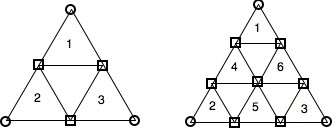
\includegraphics[width=3in]{SGf.jpg} 
   \caption{$ SG(2) $ and $ SG(3) $.  See Table~\ref{table} for notation.}
   \label{SPf}
\end{figure}

The relevant sets for $ SG(2) $ are 
\[
\mathcal{C} =\{1\dot{2}\sim 2\dot{1}, 2\dot{3}\sim 3\dot{2}, 3\dot{1}\sim 1\dot{3}\},
\quad  \mathcal{P} =\{\dot{1}, \dot{2}, \dot{3} \}, \quad  \mathcal{P} ^{1} = \mathcal{C} \cup \mathcal{P}, 
\]
and the union is disjoint. 

For $ SG(3) $ the relevant sets are 
\begin{gather*}
\mathcal{C} =\{1\dot{2}\sim 4\dot{1}, 4\dot{2}\sim 2 \dot{1}, 2\dot{ 3}\sim 5\dot{2},
5\dot{3}\sim 3\dot{2}, 3 \dot{1}\sim 6\dot{3}, 6\dot{ 1}\sim 1\dot{3}, 4\dot{ 3}\sim 5\dot{1}\sim 6\dot{2}\}, \\
   \mathcal{P} =\{\dot{1}, \dot{2}, \dot{3} \}, \quad  \mathcal{P} ^{1} = \mathcal{C} \cup \mathcal{P}, 
\end{gather*}
and the union is again disjoint. 
\end{example} 


\begin{example}[Cut square]  \label{excs} The diagram is misleading as it  is not imbedded in $ \mathbb{R}^2 $,
see \cite{Bar1}*{pp 64,65}.  

\begin{figure}[htbp] %  figure placement: here, top, bottom, or page
   \centering
   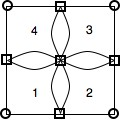
\includegraphics[width=1.2in]{cutf.jpg} 
   \caption{The cut square. See Table~\ref{table} for notation.}
   \label{cutf}
\end{figure}

Cuts are made from the centre  of a unit square to each of the 4 edges  along four intervals not including the endpoints.  More precisely, points on these intervals are counted twice.   A convenient metric is the geodesic metric.  

The relevant sets are 
\[
\mathcal{C} =\{1\dot{3}\sim 2\dot{4}\sim 3\dot{1}\sim 4\dot{2} , 1\dot{2}\sim 2\dot{1}, 2\dot{3}\sim 3\dot{2}, 3\dot{4}\sim 4\dot{3}, 4\dot{1}\sim 1\dot{4}  \},
\quad  \mathcal{P} =\{\dot{1}, \dot{2}, \dot{3}, \dot{4} \}, \quad  \mathcal{P} ^{1} = \mathcal{C} \cup \mathcal{P}, 
\]
and the union is again disjoint.
\end{example} 

%%%%%%%%%%%%%%%%%%%%%%%%%%%
\begin{example}[$ SG(2) $ with added triangle] \label{sgat} In this case $ V^{0} $ is no longer the set  of fixed points of some of the $ \psi_i $.  Moreover, in the first example $ \mathcal{C} \cap \mathcal{P} \neq \emptyset $ and in both examples $\mathcal{C} \cup \mathcal{P} \subsetneq   \mathcal{P} ^{1}  $.

The reason in each case is that the intersection $ K_i\cap K_j $ is at different relative points in $ K_i $ and $ K_j $.

\begin{figure}[htbp] %  figure placement: here, top, bottom, or page
   \centering
   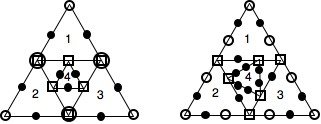
\includegraphics[width=3.5in]{intr.jpg} 
   \caption{$ SG(2) $ with added triangle. See Table~\ref{table} for notation.}
   \label{intr}
\end{figure}

In the first example the triangle 4 is equilateral and obtained from the large triangle by translation and scaling.   

In the second case triangle 4 is again equilateral but its vertices are 2/3 along the relevant side of triangles 1, 2 or 3 in the clockwise direction.  It is obtained from the original triangle by scaling, translating, and rotating 
$ \pi/6 $ in the clockwise direction.

The relevant sets in the first example are 
\begin{gather*}
\mathcal{C} =\{ 1\dot{2} \sim 2\dot{1} , 2\dot{3} \sim 3\dot{2} , 3\dot{1} \sim 1\dot{3} , 
        4\dot{1} \sim 12\dot{3}  \sim 13\dot{2} ,   4\dot{2} \sim 23\dot{1}  \sim 21\dot{3} ,   
        4\dot{3} \sim 31\dot{2}  \sim 32\dot{1} \}, \\
        \quad \mathcal{P} = \{  \dot{1}, \dot{2}, \dot{3}, 1\dot{2}\sim 2\dot{1}, 
        2\dot{3}\sim 3\dot{2}, 3\dot{1}\sim 1\dot{3}        \},  \\
     \quad \mathcal{P} ^{1} = \mathcal{C} \cup \mathcal{P}
          \cup \{ 11\dot{2}\sim 12\dot{1}, 
         13\dot{1}\sim 11\dot{3}  , 21\dot{2}\sim 22\dot{1}, 
        22\dot{3}\sim 23\dot{2},          32\dot{3}\sim 33\dot{2}, 33\dot{1}\sim 31\dot{3},\\
                 41\dot{2} \sim 42\dot{1} , 42\dot{3} \sim 43\dot{2} , 43\dot{1} \sim 41\dot{3}  \}.          
\end{gather*}         

The relevant sets in the second example are 
\begin{gather*}
\mathcal{C} =\{ 1\dot{2} \sim 2\dot{1} , 2\dot{3} \sim 3\dot{2} , 3\dot{1} \sim 1\dot{3} , 
        4\dot{1} \sim 1 \dot{3}\dot{2}    ,   4\dot{2} \sim 2 \dot{1} \dot{3},   4\dot{3} \sim 3 \dot{2} \dot{1}\}, \\
        \quad \mathcal{P} = \{  \dot{1}, \dot{2}, \dot{3},  \dot{1} \dot{2},  \dot{2} \dot{1},  
        \dot{2} \dot{3},  \dot{3} \dot{2},  \dot{3} \dot{1},  \dot{1} \dot{3}        \},   
     \quad \mathcal{P} ^{1} = \mathcal{C} \cup \mathcal{P}\cup \{ \text{``black dots''}\}.
\end{gather*}      

By taking an irrational fraction of $ 2\pi $ for the rotation in the construction of triangle 4 it is straightforward to  obtain examples where $ R $ is finite with cardinality 6, but $ \mathcal{P} $ is infinite.   
\end{example} 

%%%%%%%%%%%%%%%%%%%%%%%%%%%%%%%
\subsection{Ancestral Systems}  \label{secas} (See \cite{Kig2}*{Appendix A}.) Since $ \pi:W \to K $, where $ \pi $ is onto and continuous, $ W $ is compact and $ K $ is Hausdorff, there is a  homeomorphism  $  W/\!\! \sim\  \cong K $, where ``$ \sim $'' is the equivalence relation on $ W $ given as before by $ v \sim w$ iff $ \pi (v) =\pi (w) $.   It follows that $ K$ is determined topologically by the information $(W, \sim )$.

But we will see that for pcf structures, $ \sim $ and hence $ K$  up to homeomorphism,  can be obtained from  the \emph{combinatorial information} 
given by the \emph{finite} one-one maps $ \psi|_{V^{0}} : V^{0} \to V^{1} $ for $ i=1,\dots , M $.  This leads to the following definition.

\begin{definition}
 $ (U,V, G_1,\dots ,G_M) $ is an \emph{ancestral system}   if $U\subset V $ are finite sets, each $ G_i : U \to V $ is one-one, $ V = \bigcup_{i=1}^M G_i(U) $ and  $ G_i(U) \setminus U \neq \emptyset $ if $ U\neq \emptyset  $. 
\end{definition} 

\emph{In particular}, it follows from the relevant definitions that if   $(K,\psi_1,\dots,\psi_M)$ is a self-similar  structure then  $ (V^{0},V^{1},    \psi_1|_{V^{0}} ,\dots ,  \psi_M|_{V^{0}} ) $ is an  ancestral system.   (The case $ U=\emptyset $ in the definition corresponds to a totally disconnected fractal.) 

\medskip Conversely, one can  reconstruct a self-similar  structure from an ancestral system.  Moreover, up to the natural notions  of isomorphism for ancestral systems and isomorphism for self-similar  structures this correspondence  is one-one.  

To do this, the main point is  to  reconstruct the equivalence relation $ \sim  $  on $ W $  by using only the information in the ancestral system
$ (V^{0},V^{1},  \psi_1|_{V^{0}} ,\dots ,  \psi_M|_{V^{0}} ) $.  By a similar construction an \emph{arbitrary} ancestral system  $ (U,V,  G_1,\dots , G_M) $ will give  a self similar structure $( W/\!\! \sim, \psi_1,\dots, \psi_M )$, where $ \psi_i \circ \pi = \pi \circ i $ and   $ \pi : W\to W/\!\! \sim $  is the usual projection map.

 We use the fact that if $ w \sim v $ and $ w \neq v $ then there is a least $ n $ such that $ w|n \neq v|n $.  It follows
\[
\pi(w) = \pi(v) \in \boxed{K_{w|n} \cap K_{v|n} = V^{0}_{w|n} \cap V^{0}_{v|n}} \subset V^{n} \subset V^* , 
\]
from \eqref{kvi}.  In particular, $ w,v \in V^* $, and so in defining $ \sim $ we need only consider points in $ \mathcal{P} ^* \subsetneq W$, as all other  points belong to trivial singleton equivalence classes.

\medskip The key idea is as follows:  For $ w\neq v \in W $  set $ w = u \hat{w} $ and $ v = u \hat{v} $ where $ u $ is the maximum common initial segment.  Then $ w \sim v $ iff $   \hat{w} $ and   $  \hat{v} $ are different addresses of the same point in~$ V^{1} $.

Moreover, the set $ \mathcal{A}_x $ of all addresses of any point $ x \in V^{1} $  can be obtained by chasing backwards into $ V^{0} $ via the $ \psi_i^{-1}$. That is, $ w \in \mathcal{A}_ x $ 
 iff for some $ (x_n)_{n\geq 1} \subset V^{0} $, 
\[
x = \psi_{w_1}(x_1) = \psi_{w_1w_2}(x_2) = \psi_{w_1w_2w_3}(x_3) =  \cdots .
\]

%

%In particular, $ \sim $ is trivial except on $ \mathcal{P} ^* = \bigcup_{m\geq 1} \mathcal{P} ^{m}   \subset W$, and so we only need define $ \sim $ on $   \mathcal{P} ^* $. 
%Moreover,  the equivalence relation $ \sim $ restricted to $ \mathcal{P} ^* $ can be recovered from the information
%\[
%\psi_i : V^{0} \to V^{1} , \quad \psi_i \text{ is one-one}, \quad V^{1} = \bigcup_{i=1}^N \psi V^{0} .
%\]
%as follows.

%First suppose $ x \in V^{1}$.  Then $ w = w_1w_2 \dots $ is an address for $ x $, and we write $ w \in \mathcal{A}_x $, iff for some $ (x_n)_{n\geq 1} \subset V^{0} $, 
%\[
%x = \psi_{w_1}(x_1) = \psi_{w_1w_2}(x_2) = \psi_{w_1w_2w_3}(x_3) =  \cdots .
%\]
%All addresses $ w \in \mathcal{A}_x $ are equivalent and this defines $ \sim $ on $ \mathcal{P} ^{1} $. 

%For  $ x\in V^{(n+1)}\setminus V^{n}$, distinct addresses  are of the form $ vw $ and $ v \hat{w} $, 
%for some $ v \in W_n $ and $ w,\hat{w}\in \mathcal{A}_x $ for some $ x \in V^{0} $.  

%This then gives $ \sim $ on $ \mathcal{P} ^* $  and hence on $ W$.

\medskip
 For an arbitrary ancestral system $ (U,V, G_1,\dots ,G_M) $ we similarly define $ \sim $.  That is, for each $ x\in V $ first define $ w \in  \mathcal{A}_ x \subset W $ iff for some $ (x_n)_{n\geq 1} \subset U $, 
\[
x = G_1 (x_1) =G_1G_2 (x_2) = G_1G_2G_3(x_3) =  \cdots .
\]
Then define
$ w \sim  v $ iff
\begin{enumerate}

\item $ w=v $, or
\item $ w = u \hat{w} $ and $ v = u \hat {v} $ where, $ u \in W_n $ for some $ n\geq 0 $,  and $ \hat{w} , \hat{v}\in \mathcal{A}_x $ for some $ x \in V$.
\end{enumerate}  

%%%%%%%%%%%%%%%%%%%%%%%%%%%%%%%%%%%%%
%%%%%%%%%%%%%%%%%%%%%%%%%%%%%%%%%%%%%
%%%%%%%%%%%%%%%%%%%%%%%%%%%%%%%%%%%%%
%%%%%%%%%%%%%%%%%%%%%%%%%%%%%%%%%%%%%

\section{\textbf{Replication of a Network}}\label{secrt}

\subsection{Notation}\label{secnotr}
Let    $  (K,\psi_1,\dots, \psi_M) $ be a  pcf structure.

Let $ V^{m} $ be the set of level $ m $-boundary points as in Section~\ref{secsubss}.   

\medskip Let $ (r_{xy})_{x,y\in V^{0}} $ be a set of resistances defining  a network on $ V^{0} $,   where we allow $ r_{xy} =+\infty$ as usual.  Equivalently, let $ A=(a_{xy})_{x,y\in V^{0}} $ be the conductance matrix.  That is, $  a_{xy} = r_{xy}^{-1} $ if $ x\neq y $,  and  $ a_{xx} = -\sum \{ a_{xy} : y \neq x \} $ for fixed  $ x \in V^{0} $. 


Let $ \mathcal{E} = \mathcal{E} ^{0} $ be the corresponding Dirichlet form on $ V^{0} $. That is
\begin{equation} \label{}
\boxed{ \mathcal{E} ^{0} (f) = \mathcal{E} (f) = \frac{1}{2} \sum_{x,y\in V^{0}} a_{xy} \big(f(x) - f(y)\big)^2.}
\end{equation} 

\medskip   Let $\rho =  (\rho_1,\dots, \rho_M) $ be  a \emph{resistance scaling} vector  of positive numbers. Typically $ \rho_i > 1 $. 

The idea is that the resistance scaling factor $ \rho_i $ is the amount by which resistance distances are multiplied when going from the smaller $  K_i $ to the larger $ K $.  This is consistent  with length scaling and mass scaling, both of which are  greater than $ 1 $.  Notice that $ \rho $ is also \emph{conductance} scaling when passing in the \emph{opposite} direction from $ K $ to $ K_i$.%
\footnote
{The resistance scaling vector $ \rho $ here  is the same as the vector $\rho (    {r_1}^{-1},\dots,  {r_M}^{-1}) $ in   \cite{Bar1}*{Section 6}.  There,  $ \rho $ is a \emph{scalar} called  the \emph{resistance scaling factor}  and $( r_1 ,\dots, r_M ) $ is called the \emph{resistance vector}. See \cite{Bar1}*{p 92, Definition 6.26; p 79, before Definition 6.1}.}

 
For the IFS corresponding to $ SG(2) $ the natural value is $ \rho = (\frac{5}{3}, \frac{5}{3}  , \frac{5}{3} ) $ and for $ SG(3) $ it is $   \rho = (\frac{15}{7}, \dots  , \frac{15}{7} ) $.   See Example~\ref{extn} in Section~\ref{secctn}.
 

In this and other cases where $ \rho_1 = \dots = \rho_M $ we also use $ \rho $ to denote the individual elements of the vector $  (\rho_1,\dots, \rho_M) $.  

\medskip For $ f:V^{n} \to \mathbb{R} $ and $ w \in W_n $, define 
\begin{equation} \label{}
f_w = f\circ \psi_w:V^{0} \to \mathbb{R}.  
\end{equation} 
Thus $ f_w $ is essentially the restriction of $ f $ to the cell $ V^{0}_w $,  but  interpreted as a function defined on the domain $  V^{0} $ (which is independent of $ w $).  


%%%%%%%%%%%%%%%%%%%%%%%%%%%%%%
\subsection{Definition of Replication}  \label{secdfr}   We now  use the $ \psi_i$ and $  \rho_i $ to make  weighted copies of the network on $ V^{0} $, which are then joined together at the ramification points $ R = \bigcup_{i\neq j}V_i^{0} \cap V_j^{0} $ (see \eqref{dfpcs} and~\eqref{kvi}) to give a network on $ V^{1} $ (see~\eqref{defvn}). 


More precisely, the replicated Dirichlet form $ \mathcal{E} ^R $ and replicated conductance matrix $ A^R = (a^R_{xy})$ on $ V^{1} $ are defined by
\begin{align}
\mathcal{E} ^R (f) &= \sum_{i=1}^M   \rho_i \mathcal{E} (f_i ), \quad \text{where } f:V^{1} \to \mathbb{R} ,\label{repen}\\
a^R_{xy}&= \sum  \{\rho_i a_{uv} : \psi_i(u) = x, \ \psi_i(v) = y \}.\label{repmat}
\end{align} 
(In the sum defining $ a^R_{xy} $ there may be more than one term.  This occurs in the case of the cut square  in Example~\ref{excs}.)

It follows from the definitions that $ A^R $ is a conductance matrix and that $ \mathcal{E} ^R $ is the associated Dirichlet form.  That is,
\begin{equation} \label{}
\mathcal{E} ^R(f) = \frac{1}{2} \sum_{x,y \in V^{1}} a^R_{xy} \big(f(x) - f(y)\big)^2.
\end{equation} 



%

%Suppose  for $ 1 \leq m \leq M $ that $ V^{0} \subset W^m $ where $ W^m $ is finite  and $ (W^m,A^m) $ is a network with conductance matrix $ A^m = (a^m_{xy}) $. Let $ \mathcal{E}_m $ be the  Dirichlet form on $ (W^m,A^m) $.

%
% In particular, the case $ W^m= V^{0} $ for all $ m $ is important.  
% 
%\medskip
% \emph{Assume} for $ m \neq n $ that 
%\begin{equation} \label{wint}
% \psi  _m (W^m) \cap \psi  _n (W_n) =  \psi  _m (V^{0}) \cap \psi  _n (V^{0}) .
%\end{equation} 
%Thus copies of   $ W^m $ are   joined together by joining   the corresponding copies  of $ V^{0} $ in the standard manner  to form $ V^{1} $, but no other nodes are joined.
%This is true, for example,  if $ W^m\subset E$, where $ E $ is the set used in the Definition from  Section~\ref{secdfpcf} after replacing $ F^ \lambda $ by $ F $.
%  
%\medskip   Informally, the  \emph{replication network  $(W^R , A^ R ) $       using $ (F,\rho ) $} is obtained by
%multiplying the conductances   $ a^m_{xy} $ by $ \rho_m   $, applying    $ \psi   _m $ to   $ W^m $, and joining the resulting networks together at their common vertices (which form the critical subset of $ V^{1}$).
%Note that 
%\begin{equation} \label{} 
%V^{0} \subset W^m\ \forall m , \quad V^{0} \subset V^{1}\subset W^R.
%\end{equation} 
%The \emph{corresponding Dirichlet form} on $ (W^R,A^R) $ is denoted by~$ \mathcal{E} ^R = \mathcal{E} _A^R$.

% \medskip More precisely:
%\begin{defn}  The  \emph{replication network  $(W^R , A^ R ) $       using $ (F,\rho ) $} is given  by
%\begin{equation} \label{dfrn}
%\begin{aligned}
%W^R  &  = \bigcup_{m=1}^{M } \psi  _ m (W^m),\\
% a_{xy} ^R  &= 
% \begin{cases}
%       \rho _m a^m_{vw} & 
%       \text{if }  x\neq y,\ v,w\in V^{0}, \  \psi  _ m(v) = x,\   \psi _ m(w) = y \\
%            0                                    & \text{otherwise},
%            \end{cases} \\
%  a_{xx}^R  &= \sum\{\rho   _m a^m_{vv} :  \psi  _ m(v) = x  \}.
%  \end{aligned}
%  \end{equation} 
%  \end{defn} 
%Concerning the definition of $ a_{xy}^R $, note that by assumption there is at most one  $ m $ and one pair $ {v,w} $ satisfying the condition used in the  definition of $ a_{xy}^R  $.   Concerning $ a^R_{xx} $, there will be more than one  $ m $ and $ v $ precisely when $ x $ is in the critical set.
  
  
  %%%%%%%%%%%%%%%%%%%%%%%%%%%%%%%%%% 
\subsection{Invariance under Replication} \label{secir}
  \begin{definition} Suppose $ (K,\psi_1,\dots, \psi_M) $ is a pcf system, with sets $ V^{0} $ and $ V^{1} $, and resistance scaling vector $ \rho = (\rho_1,\dots, \rho_M ) $,  as in Section~\ref{secnotr}.  Then a network $ A $ on $  V^{0} $ is \emph{invariant under replication} (using   $ \rho$) followed by tracing if
 \begin{equation} \label{dfir}  
 \boxed{A = \Tr (A^R\mid V^{0}),}
 \end{equation} 
  where $ A^R $ is the replicated network on $  V^{1} $.
 \end{definition}

It follows from Section~\ref{sectdf} that 
\begin{proposition} $ A $ is invariant under replication followed by tracing iff the replicated Dirichlet form $ \mathcal{E} ^R $ satisfies
\begin{equation} \label{} 
\mathcal{E} (f)  = \mathcal{E} ^R(\widetilde{f}) = \min\{\mathcal{E} ^R (h) : h|_{V^{0}}  = f \},\quad 
\text{i.e.\ } \boxed{ \mathcal{E} = \Tr ( \mathcal{E} ^R \mid V^{0} )}.
  \end{equation} 
   where $ \widetilde{f} $ is the (unique) harmonic extension of $ f $ to $ V^{1} $.
\end{proposition}   
  
  
  \begin{example} \label{extn2} For $ SG(2) $ the network $ A $ on $ V^{0} $ with $ a_{ij} = 1 $  (or any fixed positive constant) for $ i\neq j $ is invariant if $ \rho = (\frac{5}{3}, \frac{5}{3}, \frac{5}{3}  ) $.  This follows from the discussion in  Example~\ref{extn}.
  
  Similarly, for $ SG(3)$ the same network $ A $ is invariant if $ \rho = (\frac{15}{7}, \frac{15}{7}, \frac{15}{7}, \frac{15}{7}, \frac{15}{7}, \frac{15}{7} ) $.
  
  We usually just write $ \rho = 5/3  $ or $ \rho = 15/7 $ respectively.

  \end{example} 
  
  
  %%%%%%%%%%%%%%%%%%%%%%%%%%%%%%%%%% 
\subsection{Finding Invariant Networks}  \label{secfin} Motivated by Example~\ref{extn2} we have the following method.

\bigskip \noindent  \emph{General procedure}: Suppose $ (K,\psi_1,\dots,\psi_M ) $ a pcf structure.
\begin{enumerate}

\item Begin with a conductance matrix $ A $ on $ V^{0} $ which reflects certain geometric or other features of $ K $, following the idea  in Examples~\ref{extn} and~\ref{extn2},   

\item Select   a putative resistance scaling vector $\widehat{\rho} = (\widehat{\rho}_1 ,\dots, \widehat{\rho}_M) $ which reflects the \emph{relative} ``resistance'' sizes (after taking inverses of the $\widehat{\rho}_i $) of the $ V_i^{0} $,   and assemble  the replicated conductance matrix $ \widehat{A}^R $ on $ V^{1} $ as in \eqref{repmat} or equivalently~ \eqref{repen}.  

\item Compute the trace conductance matrix $ \widehat{B} = \Tr (\widehat{A}^R\mid V^{0}) $ on $ V^{0} $   as in~\eqref{mtr} or by the methods in Section~\ref{seccer}.

\item \emph{Suppose} 
\begin{equation} \label{nle} 
 \Tr (\widehat{A}^R\mid V^{0}) = \lambda A \quad \text{for some } \lambda . 
\end{equation} 
\end{enumerate} 

It follows that the resistance scaling vector $ \rho  := \lambda ^{-1}\widehat{\rho} $   gives the replicated conductance matrix $ A^R = \lambda ^{-1}\widehat{A}^R$ and the trace matrix $ B = \lambda ^{-1} \widehat{B} $. 
For this $ \rho $, $    \Tr (A^R\mid V^{0}) = A$  and so  \emph{$ A $ is invariant under replication using the resistance scaling vector~$ \rho =  \lambda ^{-1}\widehat{\rho}$}.

The eigenvalue $ \lambda  $ for $ \widehat{\rho} $ is used  to give a new resistance scaling vector $ \rho $ for which the eigenvalue is $ 1$.  Thus $ \rho = (\rho_1,\dots, \rho_M) $ reflects the \emph{absolute} ``resistance'' sizes of the $ V_i^{0} $.%
\footnote{\emph{Note}:  The map $ A \mapsto  \Tr (A^R\mid V^{0})$ is nonlinear, but it \emph{is} homogeneous.  That is, if all conductances $ a_{xy} $ are multiplied by the same scalar $ \alpha $ then $ \Tr (A^R\mid V^{0})$ is also multiplied by $ \alpha$.
If $ A $ is invariant under $ \rho $ then so is any scalar multiple of $ A $.}    



\bigskip \noindent  \emph{More General procedure}: 
\begin{enumerate}
\item Begin with a class $ \mathcal{A} $ of conductance matrices  $ A $ on $ V^{0} $ which reflect  certain geometric or other features of $ K $.  

\item Using  a putative resistance scaling vector $\widehat{\rho} = (\widehat{\rho}_1 ,\dots, \widehat{\rho}_M) $ which reflects the \emph{relative} ``resistance'' sizes of the $ V_i^{0} $ but is \emph{independent} of $ A \in \mathcal{A} $,   assemble  the replicated conductance matrices $ \widehat{A}^R $ on $ V^{1} $ for $ A \in \mathcal{A} $.  

\item Compute the trace conductance matrices $ \widehat{B} = \Tr (\widehat{A}^R\mid V^{0}) $ on $ V^{0} $   as in~\eqref{mtr} or by the methods in Section~\ref{seccer}.

\item  Compute  those  $A \in \mathcal{A} $ for which there exists $\lambda > 0 $ such that 
\begin{equation} \label{}
      \Tr (\widehat{A}^R\mid V^{0})  =  \lambda A.
\end{equation} 
\end{enumerate} 


As before, the $ A $ found in (4) are invariant under the resistance scaling vector $ \rho := \lambda ^{-1} \widehat{\rho} $.

\begin{example}
See \cite{Bar1}*{Example 6.7, p82}.   *** Summarise***
\end{example} 

 %%%%%%%%%%%%%%%%%%%%%%%%%%%%%%%%%% 
\subsection{Abstract Existence Results} 
 To prove general existence results one needs to use a fixed point argument on a suitable space of Dirichlet forms in which scalar multiples of forms are identified.
 
 
 *** Metz, Lindstrom, Barlow***







 %Example~\ref{exinv} gives an example of an invariant network if $ B = \begin{bmatrix} -2 & 1 & 1 \\ 1 & -2 & 1 \\ 1 & 1  & -2 \end{bmatrix} $.

%%%%%%%%%%%%%%%%%%%%%%%%%%%%%%%%%% 
\subsection{Replication and Trace}  
Suppose that $ (\psi_1,\dots,\psi_M) $ is a pcf structure with base sets $ V^{0} $ and $ V^{1} $.  Suppose $ ( V^{0} ,  A) $ is a network and $ (V^{1} ,A^R) $ is the replicated network using the resistance scaling vector $ \rho = (\rho_1,\dots, \rho_M) $. 

Suppose  for $ i=1,\dots, M $ there is a network $ (W^i,B^i) $ such that $ V^{0} \subset W^i $, \mbox{$ \Tr(B^i\mid V^{0}) = A $}, and $ W^i\cap W^j = V^{0} $ for $ i\neq j $.

For each $ i $, one can apply   $ (\psi_i, \rho_i) $ in the natural way to  $ (W^i,B^i) $   and so obtain the replicated network $ (W^R,B^R ) $.  The trace of this network on $ V^{1} $ is then $ (V^{1} ,A^R) $.

\medskip
  More precisely, we have the following.

\begin{proposition} \label{proptr} Suppose $ F =(\psi_1,\dots, \psi_M) $ is a pcf structure with base sets $ V^{0} $ and $ V^{1} $.   Suppose $ (V^{0},A) $ is a network and  $ \rho = (\rho_1,\dots,\rho_M) $ is a resistance scaling vector.  
Let $ (V^{1}, A^R) $ be the replicated network.

Suppose   $ (W^i,B^i) $ is a network with conductance matrix $ B^i = (b^i_{xy}) $ for $ 1 \leq i \leq M $.
Suppose   $ V^{0} \subset W^i $, $ \Tr(B^i \mid V^{0}) = A $, and $ W^i\cap W^j = V^{0} $ for $ i\neq j $.

Let $ (W^R, B^R ) $ be the replicated matrix obtained by extending $ \psi_i $ to $ W^i $ so that 
$ \psi_i(W^i) \cap \psi_j(W^j) =  \psi_i(V^{0}) \cap \psi_j(V^{0})$ for $ i\neq j $, and by    
multiplying conductances in $ B^i $ by $ \rho_i $ analogous to~\eqref{repmat}. That is,
\begin{equation} \label{dfbi} 
b^R_{xy}:= \sum  \{\rho_i b^i_{uv} : \psi_i(u) = x, \ \psi_i(v) = y \}. 
\end{equation} 
Then the matrix $ B^R $ is a conductance matrix and 
the  Dirichlet form $ \mathcal{E}_B ^R $ is given by 
\begin{equation} \label{repm}
\mathcal{E} _B^R  (f,g):= \frac{1}{2} \sum_{x,y} b_{xy}^R\big(f(x) - f(y) \big) \big( g(x) - g(y) \big) 
= \sum_{i=1}^{M  } \rho_i \mathcal{E}_{B^i} (f \circ \psi_i , g \circ \psi_i  ) .
\end{equation} 

Moreover,
\begin{equation} \label{trba1}
\Tr\left(B^R\mid V^{1}\right) = A^R.
\end{equation} 
If $ A $ is invariant, then 
\begin{equation} \label{trba2} 
\Tr\left(B^R\mid V^{0}\right) = A.
\end{equation} 
\end{proposition} 

\begin{proof} The fact $ b^R_{xy} \geq 0 $ if $ x \neq y $ and the rows of $ B^R $ sum to zero follows from \eqref{dfbi} and the analogous facts for the matrices  $ B^i $. The second equality in \eqref{repm} similarly comes from summing over the sets $ W^i$ and the definitions.

\medskip For \eqref{trba1} it is sufficient to show that if $ g : V^{1} \to \mathbb{R} $ and $ f $ is its harmonic extension to $ (W^R,B^R) $ then
\[
\mathcal{E}_A^R(g) = \mathcal{E} _B^R(f). 
\]

But $ f $ is the harmonic extension of $ g $ to $ (W^R,B^R) $  iff,  for every $ i $,  $ f\circ \psi_i $ is the harmonic extension  of $ g\circ \psi_i : V^{0} \to \mathbb{R} $ to $ (W^i,B^i) $.
To see this, consider $ x \in W^R\setminus V^{1} $ and let $ i $ be the unique integer such that $ x \in \psi_i(W^i) $, noting $ x \notin V^{1} $ implies $ x \notin \psi_i(V^{0)})\cap \psi_j(V^{0)})= \psi(W^i) \cap \psi_j(W^j) $ for $ i\neq j $.  Moreover,  $ f $ is harmonic at $ x $ iff $ f \circ \psi_f $  is harmonic at $ \psi_f^{-1}(x) $, because all relevant conductances are scaled by the same factor $ \rho_i $.

\medskip Finally
\begin{align*}
\Tr(B^R \mid V^{1}) &= A^R \quad \text{by \eqref{trba1},} \\
\Tr(A^R \mid V^{0}) &= A  \quad \text{since $ A $ is invariant,} \\
\therefore\ \Tr(B^R \mid V^{0}) &= A \quad \text{by the tower property of traces \eqref{tpp}.} \qedhere \\
\end{align*}
 \end{proof} 
 
 
%%%%%%%%%%%%%%%%%%%%%%%%%%%%%%%%
%%%%%%%%%%%%%%%%%%%%%%%%%%%%%%%%
%%%%%%%%%%%%%%%%%%%%%%%%%%%%%%%%
\section{\textbf{Sequences of Compatible Networks}} 
 
*** to mainly follow \cite{Bar1}*{94--98}, but using material already develoiped ***


%%%%%%%%%%%%%%%%%%%%%%%%%%%%%%%%
%%%%%%%%%%%%%%%%%%%%%%%%%%%%%%%%
%%%%%%%%%%%%%%%%%%%%%%%%%%%%%%%%
\section{\textbf{Dirichlet Forms on PCF Fractals}} 

*** to mainly follow \cite{Bar2}*{98--105} ***

\subsection{Review of Dirichlet Forms and Laplacians}

A network $ \mathbb{G} = (V,A) $ is given by a set $ V $ of \emph{vertices} or \emph{nodes} and a symmetric \emph{conductance matrix} $ A $ such that
\begin{equation} \label{}
\begin{aligned}
a_{xy} &=  a_{yx} \geq 0  \quad \text{if } x\neq y ,\\
a_{xx} &= -\sum_{\{y: y\neq x \}}  a_{xy}.
\end{aligned}
\end{equation} 
In particular, $\sum_y a_{xy}= 0 $ for $ x \in V $. 

For $ x\neq y $, $ c_{xy} := a_{xy} $ is called the \emph{conductance} of the edge $ xy $. One defines  $ c_{xx} = 0 $. 
The \emph{conductance of the vertex} $ x $ is $ c_x := \sum_{\{y: y \neq x \}} c_{xy}=-a_{xx}$.

We assume that the network is \emph{connected} in the sense two vertices can be connected by a sequence of edges $  xy $ such that $ a_{xy} > 0 $.


\bigskip There is a natural symmetric and irreducible Markov chain $ X $ defined by $ P^x(X_1=y) = c_{xy}/c_x $.   In this setting $ c_x $ is the relative amount of time spend at $ x $, and  more precisely the unique steady state distribution is given by $ c_x/\mathbb{C}(\mathbb{G} ) $ where $ \mathbb{C}(\mathbb{G} ) = \sum_x c_x $.  

\bigskip The \emph{Dirichlet form} $ \mathcal{E} $ is defined by 
\begin{equation} \label{defdir2}
\begin{aligned}
\mathcal{E}(f,g) &:= \frac{1}{2} \sum_{x,y} a_{xy} \big(f(x) - f(y)\big)\big (g(x) - g(y)\big)  \\
   &= - \sum_{x,y} f(x) a_{xy} g(y) = - f^TAg \quad \text{(bilinear form expression)} \\ 
   &= -\sum_x f(x) \left(\sum_y a_{xy}g(y) \right) = -\sum_x f(x)\, (Ag)(x) \quad \text{(Greens's identity)}.
   \end{aligned} 
   \end{equation} 
The equivalence of these expressions is by  simple algebra.  The first expression is independent of the diagonal values $ a_{xx} $.  To obtain the second and third expressions use the fact    $\sum_y a_{xy}= 0 $ for each $ x $.

\bigskip The bracketed term in  the third line is
\begin{equation} \label{}
\begin{aligned} 
Ag(x) &:= \sum_y a_{xy} g(y)  = \sum_y a_{xy} \big(g(y) - g(x)\big)\\
  &= c_x \sum_y \frac{c_{xy}}{c_x} \big(g(y)-g(x)\big) 
  = c_x \left(\left(\sum_y \frac{c_{xy}}{c_x}  g(y)\right) -g(x)\right)
    =: c_x   \lap^P g(x).
\end{aligned}
\end{equation}  
We say $ Ag(x) $  is the \emph{natural Laplacian} of $ g $ at $x $  and say
 $ \lap^P g(x) $ is the \emph{probabilistic Laplacian} of $ g $ at $ x $.   
 
 Note that $  \lap^P g(x) $ is the difference between a weighted average  of values of $ g $ near $ x $ and $ g(x) $ itself.  It equals $ \mathbb{E} ^x g(X_1) - g(x) $.  It also equals the total current into $ x $ if $ g $ represents voltage and current flows downhill.

 \bigskip  If $ \mu $ is a measure on $ V $ then from~\eqref{defdir2}
\begin{equation} \label{} 
\begin{gathered}
 \mathcal{E}(f,g) = - (f,\lap_\mu g )_\mu = -\sum_x f(x)\, \lap_\mu g (x) \, \mu(x) , \\
\text{where} \quad  \lap_\mu g (x) := \frac{1}{\mu(x)} Ag(x)  
\end{gathered}
\end{equation} 
is the \emph{$ \mu$-Laplacian} and $ (\cdot,\cdot)_\mu $ is the $ L^2(\mu) $ inner product. That is,   $\lap_\mu$  is defined so that Green's identity holds with the  $ L^2(\mu) $ inner product.


%%%%%%%%%%%%%%%%%%%%%%%%%%%%%%%%%%%
\subsection{Harmonic Extensions and Restrictions}
We mostly follow and extend \cite{Str}*{Section 1.3}.

\begin{figure}[htbp] %  figure placement: here, top, bottom, or page
   \centering
   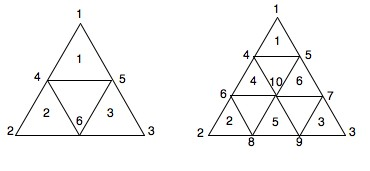
\includegraphics[width=3.5in]{SGharext.jpg} 
   \caption{$ SG(2) $ and $ SG(3) $ prefractals with vertices and 1-cells numbered.}
   \label{SGharext}
\end{figure}

\medskip
Consider a pcf structure $ (K,\psi_1,\dots ,\psi_M) $ with 0-cell $ V^{0} $ having $ N $ vertices $ (q_1,\dots, q_N) $.

%%%%%%%%%%%%%%%%%%%%%%%%%%%%%%%%%%%%
\subsubsection{Mappings on $ \mathcal{H} $}
The  space $ \mathcal{H} $ of functions defined on    $ V^* $ (or $ V^{(k)} $ or $ K $), with prescribed values on $ V^{0} $ and harmonic   elsewhere, has dimension $ N $.   Identify $ \mathcal{H} $ with $ \mathbb{R} ^N $.  The basis vector  $ e_i = (0,\dots, 1, \dots 0 )$, where the ``1'' occurs in the $ i $th position, corresponds to the harmonic function $ f $ such that $ f(q_j) = \delta _{ij} $. 



\medskip The harmonic extension of $ g : V^{0} \to \mathbb{R}$ to $ f:V^{1}\to \mathbb{R} $
can be described in terms of linear transformations or matrices
\begin{equation} \label{} 
\begin{gathered}
M_i:\mathcal{H} \to \mathcal{H},\quad   M_i :\mathbb{R} ^N \to \mathbb{R} ^N, \quad i=1,\dots M, \\
M_i(g) = f_i := f \circ \psi_i,  \quad i=1,\dots M.
\end{gathered}
\end{equation} 
In effect, $ M_i g $ is the restriction of $ f $ to $ K_i $.  Equivalently,  $ M_i g $ gives the values of $ f$ on the boundary vertices $ \psi_i(q_j) $ of $ V^{1}  $, where the $ j $th column gives the values in case $ g = e_j $. 

\begin{example}[$ SG(2) $]  Using the $ \frac{2}{5},  \frac{2}{5}, \frac{ 1}{5} $ rule for $ g = e_1 $  in Figure~\ref{SGharext}, $ f(4) = f(5) = \frac{2}{5} $ and $ f(6) = \frac{1}{5} $.  Alternatively, the values of $ f $ at vertices $ 4,5,6 $ are computed from $ -A_{HH}^{-1}A_{HG}g $ as in~\eqref{harm}.  See~\eqref{ASG2} where $ G $ corresponds to the first three rows and columns, $ H $ to the last three, and $ A_{HH}^{-1} $ is the third matrix in~\eqref{3ahh}. 

This information gives the first column of the following 3 matrices.  The other columns are similarly obtained by a symmetry argument.
\begin{equation} \label{}
M_1 = \begin{bmatrix}  1&0&0 \\ 2/5 & 2/5&1/5 \\ 2/5 & 1/5 & 2/5 \end{bmatrix}, \quad 
M_2 = \begin{bmatrix}  2/5 & 2/5&1/5 \\ 0 & 1 & 0 \\ 1/5 & 2/5 & 2/5 \end{bmatrix}, \quad 
M_3 = \begin{bmatrix}  2/5 & 1/5&2/5 \\ 1/5 & 2/5 & 2/5\\ 0 & 0 & 1 \end{bmatrix}. 
\end{equation} 
 \end{example} 
 

%%%%%%%%%%%%%%%%%%%%%%%%%%%%
\begin{example}[$ SG(3) $]  
The values of the harmonic extensions  to $ V^{1} $ of $ e_1, e_2, e_3 $ defined on $ V^{0} $  in the right side diagram from Figure~\ref{SGharext}, are given by the three columns of 
\[
-A_{HH}^{-1}A_{HG} =  \left[ \begin {array}{ccc} {\frac {8}{15}}&{\frac {4}{15}}&1/5
\\\noalign{\medskip}{\frac {8}{15}}&1/5&{\frac {4}{15}}
\\\noalign{\medskip}{\frac {4}{15}}&{\frac {8}{15}}&1/5
\\\noalign{\medskip}{\frac {4}{15}}&1/5&{\frac {8}{15}}
\\\noalign{\medskip}1/5&{\frac {8}{15}}&{\frac {4}{15}}
\\\noalign{\medskip}1/5&{\frac {4}{15}}&{\frac {8}{15}}
\\\noalign{\medskip}1/3&1/3&1/3\end {array} \right] .
\]
The rows correspond to the vertices $ 4,\dots, 10 $ in Figure~\ref{SGharext}.
See  \eqref{harm} and \eqref{ASG3}, with $ G $ corresponding to the first three rows and columns  and $ H $ to the last 7 rows and columns. Use Maple.

This gives
\begin{equation} \label{}
\begin{gathered}
M_1 = \begin{bmatrix}  1&0&0 \\ 8/15&4/15&1/5 \\  8/15 & 1/5 & 4/15 \end{bmatrix}, \  
M_2 = \begin{bmatrix}  4/15&8/15&1/5 \\ 0&1&0 \\   1/5 & 8/15   & 4/15 \end{bmatrix}, \  
M_3 = \begin{bmatrix}  4/15&1/5 & 8/15  \\   1/5 & 4/15   & 8/15  \\ 0&0&1 \end{bmatrix},   \\
M_4 = \begin{bmatrix}  8/15&4/15&1/5 \\  4/15 & 8/15 & 1/5 \\ 1/3 & 1/3 & 1/3\end{bmatrix}, \ 
M_5 = \begin{bmatrix}  1/3 & 1/3 & 1/3 \\1/5 & 8/15&4/15\\  1/5 &4/15 & 8/15   \\ \end{bmatrix}, \ 
M_6 = \begin{bmatrix}  8/15&1/5 & 4/15 \\ 1/3 & 1/3 & 1/3 \\  4/15 & 1/5 & 8/15   \end{bmatrix}.
\end{gathered}
\end{equation} 
\end{example} 

%%%%%%%%%%%%%%%%%%%%%%%%%%%%%%%%%%%%
\subsubsection{Mappings on $ \widetilde{\mathcal{H}} $}
Note that $ \mathcal{E} (u) = 0 $ precisely on the constant functions.
Factoring these out  from $ \mathcal{H}  $ one obtains an $ N-1 $ dimensional  Hilbert space $ \widetilde{\mathcal{H}}=  \mathcal{H} / \sim $ with   the energy inner product
\[
 (f,g)_\mathcal{E} = \frac{1}{2} \sum_{x,y\in   V^{0}} \big(f(x)-f(y)\big)\, \big(g(x) - g(y) \big).
 \]


A natural representative of  the equivalence class $ [g] $ is given by $g -  (\overline{g}  ,\dots, \overline{g}) $ where 
\[
\overline{g}=  N^{-1}\sum_{x\in V^{0}}g(x), \quad \text{so }  \sum_{x\in V^{0}}\big(g(x) - \overline{g}\big) = 0 .
\]




It is convenient to work with a  basis $ \epsilon_1, \dots, \epsilon_{N-1} $ for   $ \widetilde{\mathcal{H}}$ which is orthonormal w.r.t.\ the energy inner product.
%%%%%%%%%%%%%%%%%%%%%%%%%%%%
\begin{example}[$ SG(2) $]  The vectors $ (0,1,1) $ and $ (0,1,-1) $ are $ \mathcal{E} $ orthogonal and have energy norm $ \frac{1}{2} (1+1) = 1 $ and $ \frac{1}{2} (1+1+2^2) =3$ respectively.   
So we take the orthonormal basis  
\[  
\epsilon_1 = (0,1,1) \text{ or } \left(-\frac{2}{3} ,\frac{1}{3}, \frac{1}{3} \right), \quad 
\epsilon_2 =  \left(0, \frac{1}{\sqrt{3}}, -\frac{1}{\sqrt{3}}\right),
\]
where the second   representative for $ \epsilon_1 $ is the zero average representative.

It follows
\begin{align*}
M_1 \epsilon_1  &= \left[ \begin {array}{c} 0\\\noalign{\medskip}3/5\\\noalign{\medskip}
3/5\end {array} \right] =     \frac{3}{5} \epsilon_1, \quad 
M_1 \epsilon_2  =  \left[ \begin {array}{c} 0\\\noalign{\medskip}\sqrt {3}/15 
\\\noalign{\medskip}-\sqrt {3}/15 \end {array} \right] = \frac{1}{5} \epsilon _2, \quad 
\therefore\ \widehat{M}_1  = \begin{bmatrix} 3/5 & 0 \\ 0  & 1/5 \end{bmatrix};
\\
M_2 \epsilon_1  &=  \left[ \begin {array}{c} 3/5\\\noalign{\medskip}1\\\noalign{\medskip}
4/5\end {array} \right] \sim (0,2/5, 1/5) = \frac{3}{10}\epsilon_1 + \frac{\sqrt{3}}{10} \epsilon_2,
\\
M_2 \epsilon_2  &=   \left[ \begin {array}{c} \sqrt {3}/15\,\\\noalign{\medskip}\sqrt {3}/3
\\\noalign{\medskip}0\end {array} \right] \sim (0,  4\sqrt{3}/15,-\sqrt{3}/15) =
\frac{\sqrt{3}}{10} \epsilon _1 + \frac{1}{2} \epsilon_2,
\quad 
\therefore\ \widehat{M}_2  = \begin{bmatrix} 3/10 & \sqrt{3}/10 \\ \sqrt{3}/10  & 1/2 \end{bmatrix};
\\
M_3 \epsilon_1  &= 
 \left[ \begin {array}{c} 3/5\\\noalign{\medskip}4/5
\\\noalign{\medskip}1\end {array} \right] 
\sim (0,1/5,2/5) = \frac{3}{10}\epsilon_1 - \frac{\sqrt{3}}{10} \epsilon_2, 
\\
M_3 \epsilon_2  &= 
 \left[ \begin {array}{c} -\sqrt {3}/15\\\noalign{\medskip}0
\\\noalign{\medskip}-\sqrt {3}/3 \end {array} \right]
\sim (0,\sqrt{3}/15, -4\sqrt{3}/15) = -\frac{\sqrt{3}}{10} \epsilon_1 + \frac{1}{2} \epsilon_2 ,
\quad 
\therefore \widehat{M}_3  = \begin{bmatrix} 3/10 & -\sqrt{3}/10 \\ -\sqrt{3}/10  & 1/2 \end{bmatrix}.
\end{align*} 

\end{example} 

%%%%%%%%%%%%%%%%%%%%%
\begin{example}[$ SG(3) $]
With the same energy orthonormal basis $ \{\epsilon_1, \epsilon_2 \} $  as in the previous example:
\begin{align*}
M_1 \epsilon_1  &=  \left[ \begin {array}{c} 0\\\noalign{\medskip}{\frac {7}{15}}
\\\noalign{\medskip}{\frac {7}{15}}\end {array} \right] 
  = \frac{7}{15}\epsilon_1,
\quad 
M_1 \epsilon_2  =  \left[ \begin {array}{c} 0\\\noalign{\medskip}\sqrt {3}/45
\\\noalign{\medskip}-\sqrt {3}/45\end {array} \right] 
  =  \frac{1}{15}\epsilon_2, \quad 
\therefore\ \widehat{M}_1  = \begin{bmatrix}  7/15 & 0 \\ 0 & 1/15         \end{bmatrix};
\\
M_2 \epsilon_1  &=  \left[ \begin {array}{c} {\frac {11}{15}}\\\noalign{\medskip}1
\\\noalign{\medskip}4/5\end {array} \right] \sim (0, 4/15, 1/15) = \frac{1}{6}\epsilon_1 + \frac{\sqrt{3}}{10} \epsilon_2
,
\\
M_2 \epsilon_2  &=   \left[ \begin {array}{c} \sqrt {3}/9\\\noalign{\medskip}\sqrt {3}/3 \\\noalign{\medskip} 4\sqrt {3}/45\end {array}  \right] \sim (0, 2\sqrt{3}/9, -\sqrt{3}/45) = \frac{\sqrt{3}} {10}\epsilon_1 + \frac{11}{30} \epsilon_2 
 ,
\quad 
\therefore\ \widehat{M}_2  = \begin{bmatrix} 1/6 & \sqrt{3}/10\\\sqrt{3}/10 & 11/30 \end{bmatrix}
;
\\
M_3 \epsilon_1  &=  \left[ \begin {array}{c} {\frac {11}{15}}\\\noalign{\medskip}4/5
\\\noalign{\medskip}1\end {array} \right] \sim (0,1/15,4/15) = \frac{1}{6}\epsilon_1 -\frac{\sqrt{3}}{10}\epsilon_2
, 
\\
M_3 \epsilon_2  &= \left[ \begin {array}{c} -\sqrt {3}/9\\\noalign{\medskip}-
4\sqrt {3}/45\\\noalign{\medskip}-\sqrt {3}/3\end {array} \right]  \sim (0,\sqrt{3}/45, -2\sqrt{3}/9)
=   -\frac{ \sqrt{3}}{10}\epsilon_1 + \frac{11}{30}\epsilon_2     ,
\quad 
\therefore \widehat{M}_3 = \begin{bmatrix} 1/6 & - \sqrt{3}/10 \\-\sqrt{3}/10 & 11/30 \end{bmatrix};
\\
M_4 \epsilon_1  &=  \left[ \begin {array}{c} 7/15 \\\noalign{\medskip}
11/15\\\noalign{\medskip}2/3\end {array} \right] \sim (0, 4/15,1/5) 
= \frac{7}{30} \epsilon_1 + \frac{\sqrt{3}}{30} \epsilon_2 
, \\
M_4 \epsilon_2  &=   \left[ \begin {array}{c} \sqrt {3}/45\\\noalign{\medskip}\sqrt {3}/9
\\\noalign{\medskip}0\end {array} \right] \sim (0,4\sqrt{3}/45, -\sqrt{3}/45)
=   \frac{\sqrt{3}}{30}\epsilon_1+\frac{1}{6}\epsilon_2        , \quad 
\therefore\ \widehat{M}_4  = \begin{bmatrix}  7/30 & \sqrt{3}/30\\ \sqrt{3}/30 & 1/6         \end{bmatrix};
\\
M_5 \epsilon_1  &=   \left[ \begin {array}{c} 2/3\\\noalign{\medskip}4/5
\\\noalign{\medskip}4/5\end {array} \right] \sim (0,2/15, 2/15)= \frac{2}{15} \epsilon_1 ,\quad 
M_5 \epsilon_2   =   \left[ \begin {array}{c} 0\\\noalign{\medskip}4\sqrt {3}/45\\\noalign{\medskip}-4\sqrt {3}/45 
\end {array} \right]  
= \frac{4}{9} \epsilon_2 ,
\quad 
\therefore\ \widehat{M}_5   = \begin{bmatrix} 2/15 & 0 \\ 0 & 4/9 \end{bmatrix}
;
\\
M_6 \epsilon_1  &=   \left[ \begin {array}{c} 7/15\\\noalign{\medskip}2/3
\\\noalign{\medskip}11/15 \end {array} \right] \sim (0, 1/5, 4/15) = \frac{7}{30}\epsilon_1-\frac{\sqrt{3}}{30}\epsilon_2
, 
\\
M_6 \epsilon_2  &=  \left[ \begin {array}{c} -\sqrt {3}/45\\\noalign{\medskip}0
\\\noalign{\medskip}-\sqrt {3}/9\end {array} \right] \sim (0, \sqrt{3}/45,-4\sqrt{3}/45)
= -\frac{\sqrt{3}}{30}\epsilon_1 +\frac{1}{6}\epsilon_2 ,
\quad 
\therefore \widehat{M}_6 = \begin{bmatrix} 7/30 & -\sqrt{3}/{30}\\ -\sqrt{3}/{30} & 1/6 \end{bmatrix} .
\end{align*} 
\end{example} 


%%%%%%%%%%%%%%%%%%%%%%%%%%%%%%%%
%%%%%%%%%%%%%%%%%%%%%%%%%%%%%%%%
%%%%%%%%%%%%%%%%%%%%%%%%%%%%%%%%
\section{\textbf{PCF Fractals}} 

\emph{Here we follow \cite{Str}*{chapter 4}.}

%%%%%%%%%%%%%%%%%%%%
\subsection{Basic Setup}

To simplify the notation, we deal with a restricted notion of \emph{post crticially finite} [p.c.f.]\ fractals.  

\bigskip In the following assume $ K $ is invariant for the IFS $ (F_1,\dots , F_N) $ in $ \mathbb{R}^n $, where as usual the $ F_i $ are contractive.  Then
\[  
K = \bigcup_{i=1}^N F_i K .
\]
 We are interested in the \emph{connection} properties of $ K $, and the contraction ratios do not play a role.
 
 \begin{definition}[PCF fractals]
 $ K $ is \emph{p.c.f.}\  if $ K $ is connected and there exists a finite $ V_0 \subset K $ called the \emph{boundary} 
such that 
\begin{equation} \label{jucpt} 
F_i K \cap F_j K \subset F_i V_0 \cap F_j V_o \quad \text{if } i \neq j,
\end{equation} 
and 
\begin{gather*} 
V_0 \cap \bigcup_i F_i V_0  = \emptyset \\
V_0 = \{ q_1,\dots , q_{N_0} \} \text{ for some } N_0 \leq N \text{ and } F_i q_i = q_ i .
\end{gather*}
\end{definition}

\begin{remark} \mbox{}
\begin{enumerate}
\item We can reorder the $ F_i $  if necessary to obtain $ V_0 =  \{ q_1,\dots , q_{N_0} \} $. 
\item The requirement that   ``junction points'' (see later) are fixed points is not necessary and is just to simplify the exposition.  It rules out the Hata fractal.
\item Equality clearly holds in \eqref{jucpt}.
\end{enumerate} 
\hfill $\square$  \end{remark} 

\begin{definition}[Approximating Graphs]  
\begin{align*} 
&V_m  = \bigcup _i F_i V_{m-1} \text{ for } m \geq 1, \quad  
 V_*  = \bigcup_m V_m, \\
& \Gamma_0  \text{ is the  \underline{complete} \emph{graph} on } V_0, \\
& \Gamma_m  \text{ is a \emph{graph} on $ V_m $ such that:}\\
&\quad  x\sim_m y   \Longleftrightarrow \exists i \big( x = F_i x'.\ y = F_i y',\ x' \sim_{m-1} y' \big) \\
&\quad  \qquad    \,  \quad                   \Longleftrightarrow \exists w \big( |w| = m,\ x,y \in F_w V_0 \big).
\end{align*}  
\end{definition} 

\begin{definition}[Cells and junction points]  
\begin{align*}
& F_w K \text{ for $ |w|=m $ is an \emph{$  m $-cell}}. \\
& F_w V_0 \text{ is the \emph{boundary} of $ F_w K $}.\\
&\text{\emph{Junction points} are the intersection points of 2 $ m $-cells,  see \eqref{jucpt}.}
\end{align*}
\end{definition}

\begin{remark}\mbox{}
\begin{enumerate}
\item $ V_m $ is the set of all boundary points of $ m $-cells.
\item The set of junction points at level $ m $ is a subset  of $ V_m $, but not necessarily conversely. 
\item A junction point $ x $ at level $ m $ is a junction point at level $ m'>m $. The number of cells meeting at $ x $ is the same in each case.
\item $ K = \overline{V^*} $.
\item $ \Gamma_m $ captures the connectivity properties of $ K $ at level $ m $.
\end{enumerate} 
\hfill $\square$  \end{remark} 

\begin{example}
\mbox{}
\begin{enumerate}
\item $ SG(k) $ for $ k \geq 2 $.
\item  Examples in \cite{Str}*{pages 101, 102}.  These are the hexagasket, the hexagasket with smaller boundary, the Lindstrom snowflake,  polygaskets and the Vicsek set.
\end{enumerate} 
\end{example} 

%%%%%%%%%%%%%%%%%%%%%%%%%%%%%
\subsection{Energy}

We want a notion of energy $ \mathcal{E} (u) $ for certain $ u:V_* \to \mathbb{R} $, which is self-similar in the sense
\begin{equation} \label{sce} 
\mathcal{E} (u) = \sum_{i=1}^N \rho_i \mathcal{E} (u \circ F_i ) 
\end{equation} 
for certain \emph{resistance normalisation factors} $ \rho_1,\dots,\rho_N $ yet to be found.

For $ SG(2) $ and $ SG(3) $ it turns out that $ \rho = 5/3 $ and $ 15/7 $ respectively.

\subsubsection{Construction of $ \mathcal{E} $}
  We aim to achieve this by approximating $ \mathcal{E} $ by certain graph energies of the form 
\begin{equation} \label{ena} 
\mathcal{E} _m (u) = \sum_{x\sim_m y } c_m(x,y) \big( u(x) - u(y) \big)^2.
\end{equation} 
We extend this to the bilinear form 
\begin{equation} \label{} 
\mathcal{E} _m (u,v) = \sum_{x\sim_m y } c_m(x,y) \big( u(x) - u(y) \big) \big( v(x) - v(y) \big) .
\end{equation} 

\bigskip
This leads to the \emph{requirements}
\begin{align}
\mathcal{E} (u) &= \lim_{m\to \infty} \mathcal{E} _m (u) \tag{R1}\label{R1}, \\
\mathcal{E}_m(u) &= \sum_i \rho_i \mathcal{E}_{m-1} (u \circ F_i).   \tag{R2} \label{R2}
\end{align} 

 \bigskip To achieve \eqref{R2}, note \eqref{R2} implies that once we define 
\begin{equation} \label{1case} 
\mathcal{E} _0 (u) = \sum_{i< j} c_{ij} \big( u(q_i) - u(q_j) \big) ^2 ,\quad c_{ij}>0, 
\end{equation} 
and fix the $ \rho_i $, it follows that $ \mathcal{E} _m (u) $ is determined by
\begin{equation} \label{mulpr} 
\mathcal{E} _m (u) = \sum_{ |w| = m }  \sum_{i< j}  \rho_w c_{ij}  \big( u(F_w q_i) - u(F_w q_j) \big) ^2 .
\end{equation} 
Conversely, \eqref{mulpr} implies \eqref{R2}.

\bigskip
To achieve \eqref{R1} we require for $ u : V_{m-1} \to \mathbb{R} $ and $ m \geq 1 $ that 
\begin{equation} \label{minim} 
\mathcal{E}_{m-1} (u) = \min \big\{ \mathcal{E} _m (\widetilde{u}) \mid \widetilde{u} : V_m \to \mathbb{R}, \ \widetilde{u} = u \text{ on } V_{m-1}  \big\}.
\end{equation} 
Then 
\[
\mathcal{E}  _m(u)\uparrow \text{ as } m \to \infty ,
\]
and so the limit on the right of \eqref{R1} exists, though it possibly equals $ \infty $.



So now we only need to ensure by choice of the $ \rho_i $ and the $ c_{ij} $  that \eqref{minim} is satisfied in case $ m=1 $, since then it follows that \eqref{minim} is satisfied for all $ m $, essentially since the different $ m $-cells behave independently of one another.  Thus we require
\begin{equation} \label{seq} 
  \sum_{i< j} c_{ij} \big( u(q_i) - u(q_j) \big) ^2  
  =
  \sum_{k }  \sum_{i< j}  \rho_k c_{ij}  \big( \widetilde{u}(F_k q_i) -  \widetilde{u}(F_k q_j) \big) ^2,
\end{equation} 
where $ \widetilde{u} $ minimises the right side subject to $ \widetilde{u} = u $ on $ V_0 $.

The minimisation requirement, on differentiating w.r.t.\  $ \widetilde{u}(x) $ for $ x \in V_1\setminus V_0 $, gives $ \widetilde{u}(x) $ as a linear combination of the $ u(q_i) $ with coefficients determined by the $ \rho_k $ and $ c_{ij} $.  On substituting back into the RHS of \eqref{seq} we obtain a nonnegative quadratic form 
\begin{equation} \label{etil} 
\widetilde{\mathcal{E}} _1 (u) = \sum_{i< j} \widetilde{c}_{ij} \big( u(q_i) - u(q_j) \big) ^2 ,
\end{equation} 
where the $ \widetilde{c}_{ij} $ are function of the $ \rho_k $ and $ c_{ij} $.  
Thus we require
\begin{equation} \label{norm1} 
\widetilde{c}_{ij} = c_{ij} .
\end{equation} 
(We can also treat this as a nonlinear eigenvalue problem and require $ \lambda >0 $ such that 
\begin{equation} \label{ctc} 
\widetilde{c}_{ij} = \lambda c_{ij} ,
\end{equation} 
since in this case we can get \eqref{norm1} by replacing each $ \rho_k $ by $ \lambda  ^{-1} \rho_k $.)

\bigskip
\noindent \emph{Henceforth we assume   we do have \eqref{R1} and \eqref{R2}},  and hence from 
\eqref{mulpr} that 
\begin{equation} \label{coefff}
c_m(x,y) = \rho_w c_{ij}\quad  \text{if } |w|=m, \ x = F_w q_i, \ y = F_w q_j .
\end{equation}
See \cite{Str}*{pp 104, 105} for discussion.


%%%%%%%%%%%%%%%%%%
\subsubsection{Harmonic Extension Matrices}  \label{sechem} 
Suppose that $  \widetilde{u} $ is the unique minimiser of 
\[
\mathcal{E} _1 (\widetilde{u}) = \sum_{x\sim_1 y } c_1(x,y) \big( \widetilde{u}(x) - \widetilde{u}(y) \big)^2,
\]
 subject to $ \widetilde{u} = u $ on $ V_0 $.  We call $  \widetilde{u}  $ the \emph{harmonic extension} of $ u $ and say that $ u $ is \emph{harmonic}.
 
 \bigskip Recall from \eqref{coefff} that $ c_1(x,y) $ is given by
$   c_1(x,y) = \rho_k c_{ij} $ if $   x = F_k q_i $ and $ y = F_k q_j $.
 
 Differentiating w.r.t.\ $ \widetilde{u}(x) $ 
  for $ x \in V_1 \setminus V_0 $ gives $ \widetilde{u}(x) $ as a weighted sum of its neighbours, namely
\[
\widetilde{u}(x) = \frac {\sum_{x\sim_1y}   c_1(x,y) \widetilde{u}(y) } { \sum_{x\sim_1y}   c_1(x,y) }.
\]

This gives $ \# (V_1\setminus V_0) $ equations in  $ \# (V_1\setminus V_0) $ unknowns. Since the minimiser exists the equations have a solution, and so the solution is unique.  Thus   $\widetilde{u}(x) $ for $ x \in V_1 \setminus V_0 $ is a linear combination of the $ u(q_i) $.  
The averaging property implies a strict maximum principle and in particular   $\widetilde{u} $ assumes its maximum and minimum on $ V_0 $.  This also implies  
\[
\widetilde{u}(x) = \sum_{i=1}^{N_0} a_{xi} u(q_i) \text{ for } a_{xi} > 0 .
\]
***Why does Strichartz only claim $ \geq 0 $ ?? ***

We may collect this information into the $ N_0 \times N_0 $ \emph{harmonic extension matrices} $ A_i $ for $ i=1.\dots, N $ where
\[
\begin{bmatrix} 
(\widetilde{u}\circ F_i)(q_1) \\ \vdots \\ (\widetilde{u}\circ F_i)(q_{N_0}) 
\end{bmatrix}
= A_i 
\begin{bmatrix} 
u(q_1) \\ \vdots \\ u(q_{N_0}) 
\end{bmatrix}
\]
The $ A_i $ are generally not invertible.

\bigskip Substituting into \eqref{seq} we obtain a formula for \eqref{etil} and see that each $ \widetilde{c}_{ij} > 0 $.  This implies from \eqref{ctc} that each $ c_{ij}>0 $ and so we see why we needed the \emph{complete} graph $ \Gamma_0 $ on $V_0 $.  


%%%%%%%%%%%%%%%%%%%%%%%%%%%%%
\subsection{Laplacians}  \label{seclap} We assume that $ K $ is a p.c.f.\ fractal with $ \mathcal{E} _0 $ as in \eqref{1case},  $ \mathcal{E} _m (u) $ as in \eqref{R2} for $ \rho_i > 1 $ or equivalently as in \eqref{mulpr}, and such that \eqref{minim} is true.

The \emph{domain} of $ \mathcal{E} $ is 
\[
\mathcal{D} ( \mathcal{E} ) := \{ i : \mathcal{E} (u) < \infty   \}.
\]
Let
 \[
\rho = \min \rho_i , \ r = \rho^{-1}\  (< 1),\  r_w = \rho_w^{-1}.
 \]

\begin{proposition} If $ x,y \in V_* $ belong to the same or adjacent $ m $-cells then
\[
|u(x) - u(y) | \leq \frac{ 2 r ^{m/2} }{ 1 - r^{1/2} } \mathcal{E} (u)^{1/2}.
\]
This implies 
\[
|u(x) - u(y) | \leq M |x-y|^ \gamma ,
\]
where $ M $ and $ \gamma $ depend  on the Euclidean contraction constants for the $ F_i $.
\end{proposition} 

\begin{proof}
If $ x \sim_m y $ then
\[
|u(x)- u(y) | \leq r^{m/2} \mathcal{E} (u)^{1/2}.
\]
This already gives continuity.

By a simple chaining argument, see \cite{Str}*{p28}, if $ x , y \in V_*$ belong to the same or adjacent $ m $-cells, the first result follows.

The second follows by relating the contracting ratios of the $ F_i $ to $ r $.
\end{proof} 



\begin{proposition} $ \mathcal{E} $ defines a Hilbert space on $ \mathcal{D} ( \mathcal{E} )$  / constants.
\end{proposition} 

\begin{proof} Straightforward.  See \cite{Str}*{page 29}.
\end{proof} 

\begin{definition} \label{dfhar} We say that $ u \in C(K)$ is \emph{harmonic} if $ u|_{V_m} $ is the harmonic extension of $ u|_{V_{m-1}} $
for  all $ m\geq 1 $.  Note that $ u $ is completely determined by $ u|_{V_0} $. 
\end{definition} 

\begin{proposition} \label{hebl} If $ \widetilde{ u } $ and $ \widetilde{v} $ are the harmonic extensions $  \widetilde{ u } , \widetilde{v} :V_{m+1} \to \mathbb{R} $ 
of $ u,v :V_m \to \mathbb{R} $ then
\[
\mathcal{E} _{m+1}(  \widetilde{ u } ,  \widetilde{ v }  )= \mathcal{E} _m (u,v) .
\]
In fact, if $ v':V_{m+1} \to \mathbb{R} $ is any exension of $ v $ then 
\[
\mathcal{E} _{m+1}(  \widetilde{ u } ,  v'  )= \mathcal{E} _m (u,v) .
\]
\end{proposition}

\begin{proof} The first is by the polarisation identity.  The second   follows by considering $ \mathcal{E} _{m+1}(  \widetilde{ u } ,  \widetilde{ v }  - v'  )$.  See \cite{Str}*{Lemma 1.3.1, page 24}.
\end{proof} 

\begin{definition} The space $ \mathcal{S} ( \mathcal{H} _0, V_m ) $ of \emph{piecewise harmonic splines of level $ m $} consists of those functions $ u \in C(K)$ such that $ u \circ F_w $ is harmonic for $ |w|=m $.  (See Section~\ref{sechem}.)

For each $ y \in V_m $, $ \psi_y^m $ is the piecewise harmonic $ m $-spline such that $  \psi_y^m(z) = \delta _y(z) $.
\end{definition} 

That is, $ u \in \mathcal{S} ( \mathcal{H} _0, V_m ) $ is harmonic on $ K $ except on $ V_m $.  The function $ \psi_y^m $ is harmonic except on $ V_m $, and equals $ 1 $ at $ y $ and $ 0 $ everywhere else on $ V_m $. 

Note that 
\begin{enumerate}
\item $ u \in  \mathcal{S} ( \mathcal{H} _0, V_m ) $ is characterised by $ u|_{V_m} $.  $  \mathcal{S} ( \mathcal{H} _0, V_m ) $  has dimension $ \# V_m $ with basis 
 $ \{  \psi_y^m : y \in V_m \}  $.
\item $ \mathcal{E} (u ) = \mathcal{E} _m (u) $ if $  u \in  \mathcal{S} ( \mathcal{H} _0, V_m ) $.
\item The $ \psi_y^m $ form a partition of unity on $ K $. If $ y \notin K_w $ then  $ \psi_y^m =0$ on $ K_w $.
\end{enumerate} 
 

\begin{proposition} \label{p1612} $ u \in C(K) $ is approximated uniformly by $ u_m \in  \mathcal{S} ( \mathcal{H} _0, V_m ) $ such that $ u_m |_{V_m} = u|_{V_m} $.  

If $ u \in \mathcal{D} ( \mathcal{E} ) $ then $ \mathcal{E} (u_m, u) \to 0 $ as $ m \to \infty $.
\end{proposition} 

\begin{proof} Straightforward.  See \cite{Str}*{page 30}.
\end{proof} 

The \emph{effective resistance} $ R(x,y) $ on $ K $   is defined as follows.

\begin{definition}
Fix $ x,y \in V_m $.  Then
\begin{equation} \label{dfE} 
R(x,y)^{-1} := \min \{ \mathcal{E} (u) : u(x) = 0,\ u(y) = 1 \}. 
\end{equation} 
Equivalently, $ R(x,y) $ is the least value of $ R $ such that 
\[
|u(x) - u(y)|^2 \leq R\, \mathcal{E} (u) \quad \forall u \in \mathcal{D} ( \mathcal{E}  ).
\]

For $ x,y \in V_* $ it follows from the definition and the properties of harmonic minimisers that    $ R(x,y) $ is independent of $ m $ provided $ x,y\in V_m $.  This defines $ R(x,y) $ for $ x,y \in V_* $.  

It is straightforward that $ R(x,y) $ is continuous in $ x $ and $ y $, and so by continuity is defined on~$ K $. 

Moreover, it follows that \eqref{dfE}   holds for $ x,y\in K $.
\end{definition}

\begin{proposition} 
$ R $ is a metric on $ K $.
\end{proposition}

\begin{proof} It is sufficient to prove this on any finite network and then use continuity.  This is standard.
\end{proof}

\begin{proposition} Let $ x= F_w q_i $ and $ y = F_w q_j $. 
Then
\[ 
 \left(\sum_i c_{ij}\right)^{-1} r_w \leq R(x,y) \leq c_{ij}^{-1} r_w .
 \]
  Suppose $ x , y \in K$ belong to the same $ m $-cell.  Then
  \[
  R(x,y) \le c  r_ w .
  \]
 \end{proposition}
 
 \begin{proof} Suppose $ \psi_y^m $ is the piecewise harmonic $ m $-spline such that $  \psi_y^m(z) = \delta _y(z) $. Then
  \[
 R(x,y)^{-1}  \leq \mathcal{E} ( \psi_y^m ) =  \left(\sum_i c_{ij}\right)  \rho _w .
 \]
 
 Conversely, consider \emph{any} $ u $ such that  $ u(x) = 0 $ and $ u(y) = 1 $.  Then 
\[
 \mathcal{E} (u) \geq \mathcal{E} _m (u)  \geq c_{ij} \rho_w,
\]
and so $ R(x,y)^{-1} \geq c_{ij} \rho_w $.

For the second result use a chaining argument.
\end{proof}  

It follows that the resistance metric gives the Euclidean topology, but it is not normally equivalent to a power of the Euclidean metric.

\bigskip We next give a   definition of the ``weak'' $ \mu $-Laplacian w.r.t.\  a regular measure.

We use the notation $ v \in \mathcal{D} _0 ( \mathcal{E} ) $ for $ v \in \mathcal{D} ( \mathcal{E} ) $ and $ u=0 $ on $ V_0 $.

\begin{definition} Suppose $ u \in \mathcal{D} ( \mathcal{E} ) $ and $ f $ is continuous.  Then $ u \in \mathcal{D} ( \lap_ \mu ) $ and $ \lap_\mu u=f $ if 
\begin{equation} \label{wdflap}
\mathcal{E} (u,v) = - \int fv\, d\mu \quad \forall v \in \mathcal{D} _0 ( \mathcal{E} ) .
\end{equation} 
\end{definition} 

We use the notation
\begin{definition} $ \mu $ is a \emph{self-similar measure} on $ K $ if  $ \exists \mu_i > 0 $ such that
\begin{align*} 
\mu(F_w K ) = \prod_{i=1}^N \mu_{w_i} =: \mu_w .
\end{align*} 
\end{definition}

It follows that $ \mu $ has the scaling property 
\begin{equation} \label{} 
\int_K f\, d\mu = \sum_i \mu_i \int f \circ F_i \, d\mu  
\end{equation} 

The Laplacian has the following scaling property.

\begin{proposition} If $ \mu $ is a scaling measure then
\begin{equation} \label{scme}
\lap_\mu (u \circ F_w) = r_w \mu_w\,  (\lap_\mu u ) \circ F_w.
\end{equation}
\end{proposition} 

\begin{proof}
Suppose $ \lap_\mu u = f $. From the definition \eqref{wdflap} of the  $ \mu $-Laplacian, using the scaling properties \eqref{sce}  
and \eqref{scme} in the left and right sides respectively,
\[
\sum_{i=1}^N \rho_i \mathcal{E} (u \circ F_i,  v \circ F_i) 
    = -\sum_i \mu_i \int_K (f \circ F_i)   (v\circ F_i) \, d\mu  ,
    \] 
    for $ v \in   \mathcal{D} _0 ( \mathcal{E} ) $.
    
    Fix $ i $ and $ w \in \mathcal{D} _0 ( \mathcal{E} ) $.  Let $ v \circ F_i = w $ and $ v \circ F_j = 0 $ if $ j \neq i $.
    Then it follows that 
    \[
    \rho_i \mathcal{E} ( u \circ F_i, w ) = - \mu_i \int_K (f\circ F_i )\, w \, d\mu .
    \]
From \eqref{scme} it follows
\[
\rho_i \lap_\mu (u\circ F_i) = \mu_i\,  (\lap_\mu u )\circ F_i   .
\]
Iterating gives the required result. 
\end{proof} 

Informally, we may hope that harmonic functions $ u $ as in Definition~\ref{dfhar} are characterised by $ \lap_\mu u = 0 $, essentially since the measures correspond to a conformal factor at each vertex. 
This is the case, and more is true.

We introduce the pointwise Laplacians.

\begin{definition} \label{dfdl} The \emph{graph (or discrete) Laplacian} $ \lap_m $ on $ \Gamma_m $  (based on the conductances) is 
\begin{equation} \label{}
\lap_m u(x) = \sum_{y\sim_m x} c_m(x,y) \big(u(y) - u(x)\big).
\end{equation}
\end{definition}  

In the following theorem one can think of the right side of \eqref{ptlap} as a graph laplacian on $ V_m $ in which the edges $ xy $ are weighted by   $ c_m(x,y) $ and the vertices $ x $ are weighted by $  \left(\int_K \psi_x^m d\mu \right)^{-1}$.  This  \emph{modified} graph laplacian approaches the weak laplacian without any renormalisation factors. 

 Note that by the remarks preceding Proposition~\ref{p1612}, if $ \mu $ is a self-similar measure then the the denominator in the following  is simple to evaluate.  Namely
 \[
 \int_K \psi_x^m d\mu = \frac{1}{3} \sum \{ \mu_w: |w|=m,\ x \in f_w V_0 \}.
 \]
This assumes $ V_0 $ is a triangle, otherwise change the $ 3 $.
 
 
 

\begin{theorem} \label{wlll}
Suppose $ u \in \mathcal{D}  (\lap_\mu )$.  Then 
\begin{equation} \label{ptlap} 
\lap_\mu u(x) = \lim_{m\to \infty}  \frac{\lap_m u(x)} { \int_K \psi_x^m d\mu}.
\end{equation} 
and the convergence is uniform on $ V_*\setminus V_0 $.

Suppose $ u \in C(K) $ and  the right side of \eqref{ptlap} converges uniformly   on $ V_* \setminus V_0 $.  Then $ u \in \mathcal{D} (\lap_\mu) $ and \eqref{ptlap} holds.
\end{theorem}    

\begin{proof} See \cite{Str}*{Theorem 2.2.1, page 44}.

The idea is to first suppose $ x \in V_m \setminus V_0$ for $ m $ large.

Let $ \lap_\mu = f  $.  Then
\[
\mathcal{E} (u, v) = - \int_K fv\, d\mu \quad \forall   v \in \mathcal{D} _0 ( \mathcal{E} ) .
\]

Let  $ v = \psi^m_x $.  Then 
\[
\mathcal{E} (u, \psi_x^m) = \mathcal{E} _m (u, \psi_x^m) = - \lap_m u(x) ,
\]
where the first inequality comes from Proposition~\ref{hebl} and the second from the definitions of $ \lap_m u$ and $ \psi^m_x $.
Moreover,
\[
\int_K f \psi_x^m d\mu \approx f(x) \int_K \psi_x^m d\mu = \lap_\mu u(x) \int_K \psi_x^m d\mu.
\]
Hence
\[
\lap_\mu(x) \approx \frac{ \lap_m u(x) } {\int_K \psi_x^m d\mu }.
\]
\end{proof} 

\noindent \emph{Thus we can regard \eqref{ptlap} as a pointwise definition of the Laplacian $ \lap_\mu u(x) $.}
 
\begin{definition} At a boundary point $ q_i \in  V_0 $     the \emph{normal derivative} of $ u $ is defined by
\[
\partial _n u(q_i) = \lim_{m\to \infty } \rho_i^m \sum_{j\neq i} c_{ij} \big( u(q_i) - u (F_i^m q_j) \big)
= - \lim_{m\to \infty} \lap_m u(q_i),
\]
provided the limit exists.
\end{definition} 

Note the sequence is constant if $ u $ is harmonic.  *** Write out the argument ***

For the following, c.f.\ \cite{Str}*{Theorem 2.3.2.,  page 47}.

\begin{theorem}[Gauss-Green theorem]  \label{GGthm}
Suppose  $ u \in \mathcal{D} (\lap_\mu ) $.  Then $ \partial _n u(q_i)  $ exists for all $ q_i \in V_0 $.  For all $ v \in \mathcal{D} ( \mathcal{E} ) $ the following Gauss-Green formula holds:
\begin{equation} \label{}
\mathcal{E} (u,v) =  - \int_K (\lap_ \mu u ) v \, d\mu + \sum_{q_i \in V_0} v(q_i) \partial _n u(q_i).
\end{equation} 
\end{theorem}

\begin{proof} First take $ v(q_i) = 1 $ and  $   v(q_j) = 0 $ if $ j \neq i $ in \eqref{wdflap}.   
\end{proof} 

\begin{remark} Hence
\begin{enumerate}
\item $ \int_K  \lap_ \mu u    \, d\mu = \sum_{q_i \in V_0}  \partial _n u(q_i)$.
\item $   u \text{ harmonic } \Longrightarrow   \sum_{q_i \in V_0}  \partial _n u(q_i) = 0 $. 
\end{enumerate}
\hfill $\square$  \end{remark} 


*** Following Corollary to be checked***

\begin{corollary} 
If $ u \in \mathcal{S} ( \mathcal{H}  _0, V_m) $ and $ v \in \mathcal{D} ( \mathcal{E} ) $  then 
\[
\mathcal{E} (u,v) = \mathcal{E}_m (u,v)  = \sum_{|w|=m} \sum_{p \in \partial V_w } v(p) \partial_n^{F_w V_0} u(p).
\]
Moreover, for $ p = q_i  $ and $ w = i\cdots i $, 
\[
\partial_n^{F_w V_0} u(p) := \lim_{n\to \infty} - \lap_n u(p) = - \lap _m u(p) .
\]
A similar result applies to every $ F_w V_0 $.
\end{corollary} 

\begin{proof}
The first equality is from Proposition~\ref{hebl} but going from $ V_m $ directly to $ V_M $ for $ M>m $ rather than from $ V_m $ to $ V_{m+1} $. 

Equality between the first and third quantities is from Theorem~\ref{GGthm} applied to each $ F_w V_0 $ separately.

For the last assertion, the sequence is constant for $ n \geq m $ by the harmonicity of $ u $ in  $ F_w V_0 $, and we have just taken the $ m $th member of the sequence.  This requires that the appropriate e-value of the harmoni extension matrix is the renormalisation constant.  See \cite{Str}: page 26, last paragraph before exercises;  page 48, Figure 2.3.1
\end{proof} 


\bigskip *** Summarise the material on 
 Greens function,  on pages 116--119 of \cite{Str}. ***


\bigskip *** Summarise the material on non self-similar fractals on  on pages 122--124 of \cite{Str}. ***


%%%%%%%%%%%%%%%%%%%%%%%%%%%%%%%%
%%%%%%%%%%%%%%%%%%%%%%%%%%%%%%%%
%%%%%%%%%%%%%%%%%%%%%%%%%%%%%%%%
 \section{Hiearchical Fractals}
 
 We consider a fractal built as a limit of scaled copies of the $ SG(2) $ and $ SG(3) $ prefractals, see Figure~\ref{SGnon}.
 
 \begin{figure}[htbp] %  figure placement: here, top, bottom, or page
    \centering
    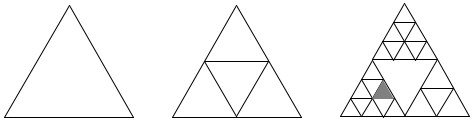
\includegraphics[width=3.5in]{SGnon.jpg} 
    \caption{Prefractals for a hierarchical gasket; $ \Gamma_0 $, $ \Gamma_1 $ and $ \Gamma_2 $ from left to right.}
    \label{SGnon}
 \end{figure}
 
 \begin{remark}[Basic set up]  \mbox{}
 \begin{enumerate}
 \item $ \Gamma_0 $ is the complete graph on $ V_0 $, which has 3 vertices.
 \item $ V_0 \subset V_1 \subset V_2 \subset \cdots $,    $ V_* = \bigcup_m V_m $.
 \item $ V_* $ is dense in $ K $.
 \item $ V_m $ and $ K $ are partitioned into overlapping $ m $-cells, each with 3 boundary points in $ V_m $.
 \item $ x\sim_m y $ if $ x $ and $ y $ are in a common $ m $-cell.
 \item If $ C $ is an $ m $-cell then the way the parent $ m-1 $ cell    is subdivided is given by $ n (C) $,  where $ n(C) = 2 , 3 $ according as $ C $ is part of a scaled copy of $ SG(2) $ or $ SG(3) $ respectively.
 
 Thus if $ C $ is the top 1-cell in $V_1 $ from Figure~\ref{SGnon} then $ n(C) = 2 $; if it is the shaded cell then $ n(C) = 3 $. 
  \end{enumerate} 
 \hfill $\square$  \end{remark} 
 
 \begin{definition} $ K $ as constructed above is a \emph{hierarchical gasket}.  If $ n(C) $ depends only on the level of $ C $ then 
 $ K $ is a \emph{homogeneous hierarchical gasket}.
 \end{definition}
 
 
 \begin{remark}[Words and other Notation]\mbox{}
 \begin{enumerate}
 \item Consider words $ w = w_1w_2w_3\dots $ which may be finite or countably infinite in length.  Here $ w_i \in \{1,2,3\} $ or $ \{1,2,\dots, 6\} $.
 \item  Cells at level $ m $ are denoted $ C_w $ with length $ |w| = m $.  The cell at level $ 0 $ is denoted $ C_\emptyset $.
 
 The shaded 2-cell in Figure~\ref{SGnon}   is $ C_{14} $, using the convention of numbering the maps corresponding to $ SG(2) $ and $ SG(3) $ in a counterclockwise manner beginning from the bottom left ``corner''.
 \item $ w_m \in    \{1,2,3\} $ or $ \{1,2,\dots, 6\} $ according as $n( C_{w_1\dots w_{m}}) = 2 $ or $ 3 $ respectively.  
  \end{enumerate} 
\hfill $\square$  \end{remark} 


\begin{remark}[Renormalisation Factor]  The cell $ m $-cell $ C_w $ is given the \emph{conductance renormalisation factor} 
$ \rho_w = \rho_{w_1}\cdot \ldots \cdot \rho_{w_m} $ where $ \rho_{w_i} = 5/3 $ or $ 15/7 $ according as $ n(C_{w_1\dots w_{i}})=2 $ or 3 respectively.

That is, one multiplies by 5/3 or 15/7 according as the cell belongs to a scaled copy of $ SG(2) $ or $ SG(3) $ respectively.  Corresponding to the shaded cell $ C_{14} $, $ \rho_{14} = \frac{5}{3} \times \frac{15}{7} $.

Thus 
\[
\rho_w = \left(  \frac{5}{3} \right)^{m_2} \times \left( \frac{15}{7} \right)^{m_3} .
\]
where $ m_2 $ is the number of occurrences of 2 among $ n(C_{w_1\dots w_{i}}) $ for $ 1\leq i \leq m $, and $ m_3 $ is the number of occurrences of 3.

The \emph{resistance renormalisation factor} is $ r_w := \rho_w^{-1} $.
\hfill $\square$  
\end{remark} 


\begin{remark}[Energy]  The \emph{energy functional} on $ V_m $ is defined by
\[
\mathcal{E} _m (u) = \sum_{|w|=m} \sum_{x\sim_m y} \rho_w \big( u(x) - u(y) \big)^2 .
\]
It follows 
\begin{equation} \label{} 
\mathcal{E} _m (\widetilde{u})  = \mathcal{E} _{m-1}(u) 
\end{equation} 
where $ \widetilde{u} $ is the harmonic extension to $ V_m $ of $ u :V_{m-1} \to \mathbb{R} $.

Moreover,
\begin{equation} \label{}
\mathcal{E} _m(u) \uparrow \text{ as } m \to \infty , \quad \mathcal{E} (u) := \lim_{m\to \infty } \mathcal{E} _m (u) 
\end{equation}
exists (possibly as $ \infty $) for $u :V_* \to \mathbb{R} $ and  hence similarly for $ u \in C(K) $.
\hfill $\square$  

\end{remark}


\begin{remark} The properties of energy and harmonic functions in Section~\ref{seclap} all hold, except for the scaling properties.

In particular, the diameter of a cell $ C_w $ in the resistance metric is comparable to $ r _w $.
\hfill $\square$ 
 \end{remark}


\begin{remark}[Laplacian]  Let $ \mu $ be the standard measure with 
\[
 \mu(C_w) = \mu_w  = \left(  \frac{1}{3} \right)^{m_2} \times \left( \frac{1 }{6} \right)^{m_3} ,
 \]
 although any other measure is similar.  
 
 The \emph{discrete Laplacian} for $ x \in V_m $ is 
 \[
 \lap_m u(x) = \sum_{y\sim_m x} c_m(x,y) \big( u(x) - u(y) \big),
 \]
where $ c_m(x,y) = \rho_w $ if $ x,y \in C_w $,  c.f.\  Definition~\ref{dfdl}.

 The \emph{weak Laplacian} is
 \[ 
 \lap_\mu u(x) = \lim_{m\to \infty}  \frac{\lap_m u(x)} { \int_K \psi_x^m d\mu},
\]
by the same proof as in  Theorem~\ref{wlll}.
 
 It is straightforward to show that for $ x \in V_m $,
 \[
 \int_K \psi_x^m d\mu = \sum_j \frac{1}{3} \mu_{w^j} 
  \] 
 where $ C_{w^j} $  are the $ m $-cells containing $ x $,  of which there are 1, 2 or 3.  If $ x \in V_m \setminus V_{m-1} $ then all the $ \mu_{w^j} $ are equal.
 \hfill $\square$  \end{remark}


*** Include the material on Greens function on page 124 of \cite{Str}.  Also Prop 1.9 and Theorem 1.12 of  \cite{KL}. ***

 



%%%%%%%%%%%%%%%%%%%%%%%%%%%%%%%%
%%%%%%%%%%%%%%%%%%%%%%%%%%%%%%%%
%%%%%%%%%%%%%%%%%%%%%%%%%%%%%%%%
\newpage
\begin{thebibliography}{9} 

\bib{Bar3}{article}{
   author={Barlow, Martin T.},
   title={Heat kernels and sets with fractal structure},
   conference={
      title={},
      address={Paris},
      date={2002},
   },
   book={
      series={Contemp. Math.},
      volume={338},
      publisher={Amer. Math. Soc.},
      place={Providence, RI},
   },
   date={2003},
   pages={11--40},
%   review={\MR{2039950 (2005e:60166)}},
}
	

\bib{Bar1}{article}{
   author={Barlow, Martin T.},
   title={Diffusions on fractals},
   conference={
      title={Lectures on probability theory and statistics},
      address={Saint-Flour},
      date={1995},
   },
   book={
      series={Lecture Notes in Math.},
      volume={1690},
      publisher={Springer},
      place={Berlin},
   },
   date={1998},
   pages={1--121},
%   review={\MR{1668115 (2000a:60148)}},
}

\bib{Bar2}{article}{
   author={Barlow, Martin T.},
   title={Random Walks on Graphs},
   conference={
        title = {RIMS},
      date={2005},
   },
   date={2005},
   pages={1--29},
}


\bib{Kam}{article}{
   author={Kameyama, Atsushi},
   title={Distances on topological self-similar sets and the kneading
   determinants},
   journal={J. Math. Kyoto Univ.},
   volume={40},
   date={2000},
   number={4},
   pages={601--672},
%   issn={0023-608X},
%   review={\MR{1802840 (2001m:37024)}},
}



\bib{Kig2}{article}{
   author={Kigami, Jun},
   title={Harmonic calculus on p.c.f.\ self-similar sets},
   journal={Trans. Amer. Math. Soc.},
   volume={335},
    date={1993},
   number={2},
   pages={721--755},
%   issn={0002-9947},
%   review={\MR{1076617 (93d:39008)}},
}
		



\bib{Kig}{book}{
   author={Kigami, Jun},
   title={Analysis on fractals},
   series={Cambridge Tracts in Mathematics},
   volume={143},
   publisher={Cambridge University Press},
%   place={Cambridge},
   date={2001},
   pages={viii+226},
%   isbn={0-521-79321-1},
%   review={\MR{1840042 (2002c:28015)}},
}
		
\bib{Str}{book}{
   author={Strichartz, Robert S.},
   title={Differential equations on fractals},
%   note={A tutorial},
   publisher={Princeton University Press},
%   place={Princeton, NJ},
   date={2006},
   pages={xvi+169},
%   isbn={978-0-691-12731-6},
%   isbn={0-691-12731-X},
%   review={\MR{2246975 (2007f:35003)}},
}
	

\end{thebibliography}

\end{document} 

